\documentclass[article]{jss}
\usepackage[utf8]{inputenc}
% \usepackage{draftwatermark}
% \SetWatermarkText{Draft}
% \SetWatermarkScale{2}
\newif\ifen
\newif\ifes
\newcommand{\en}[1]{\ifen#1\fi}
\newcommand{\es}[1]{\ifes#1\fi}
\entrue
\usepackage[utf8]{inputenc}
\usepackage{paracol}
%\newcommand{\jan}{%
%  \en{January}%
%  \es{Enero}
%}

\newcommand\Wider[2][3em]{%
\makebox[\linewidth][c]{%
  \begin{minipage}{\dimexpr\textwidth+#1\relax}
  \raggedright#2
  \end{minipage}%
  }%
}

\usepackage{wrapfig}
\usepackage{caption}
\usepackage{subcaption}
\usepackage{amsmath} %para escribir funci\'on partida , matrices
\usepackage{amsthm} %para numerar definciones y teoremas
\usepackage{amsfonts} % \mathbb{N} -> conjunto de los n\'umeros naturales
\usepackage{bm} % \bm{\alpha} bold greek symbol
\usepackage[makeroom]{cancel} % \cancel{} \bcancel{} etc
\usepackage{mdframed}
\usepackage{algorithm}
\usepackage{comment}
%\usepackage{quoting}
\usepackage{mathtools}
\usepackage{tikz}
\usepackage{csvsimple}
\usepackage{listings}
\renewcommand{\lstlistingname}{Code}% Listing -> Algorithm
\usepackage{todonotes}
\usepackage[binary-units]{siunitx}

 % by: https://tex.stackexchange.com/questions/87940/weird-warning-using-pdfx
\RequirePackage{pdf14}

% by: https://tex.stackexchange.com/questions/74636/mla-package-and-thumbpdf
\makeatletter
\@namedef{ver@thumbpdf.sty}{}
\makeatother

\definecolor{dkgreen}{rgb}{0,0.6,0}
\definecolor{mauve}{rgb}{0.58,0,0.82}

\definecolor{julia}{rgb}{1, 0.5, 1}
\definecolor{python}{rgb}{1, 1, 0.5}
\definecolor{r}{rgb}{0.65, 0.65, 1}
\definecolor{all}{rgb}{0.85, 0.85, 0.85}



% tikzlibrary.code.tex
%
% Copyright 2010-2011 by Laura Dietz
% Copyright 2012 by Jaakko Luttinen
%
% This file may be distributed and/or modified
%
% 1. under the LaTeX Project Public License and/or
% 2. under the GNU General Public License.
%
% See the files LICENSE_LPPL and LICENSE_GPL for more details.

% Load other libraries

%\newcommand{\vast}{\bBigg@{2.5}}
% newcommand{\Vast}{\bBigg@{14.5}}
% \usepackage{helvet}
% \renewcommand{\familydefault}{\sfdefault}

\usetikzlibrary{shapes}
\usetikzlibrary{fit}
\usetikzlibrary{chains}
\usetikzlibrary{arrows}

% Latent node
\tikzstyle{latent} = [circle,fill=white,draw=black,inner sep=1pt,
minimum size=20pt, font=\fontsize{10}{10}\selectfont, node distance=1]
% Observed node
\tikzstyle{obs} = [latent,fill=gray!25]
% Invisible node
\tikzstyle{invisible} = [latent,minimum size=0pt,color=white, opacity=0, node distance=0]
% Constant node
\tikzstyle{const} = [rectangle, inner sep=0pt, node distance=0.1]
%state
\tikzstyle{estado} = [latent,minimum size=8pt,node distance=0.4]
%action
\tikzstyle{accion} =[latent,circle,minimum size=5pt,fill=black,node distance=0.4]
\tikzstyle{fijo} =[latent,circle,minimum size=5pt,fill=black]


% Factor node
\tikzstyle{factor} = [rectangle, fill=black,minimum size=10pt, draw=black, inner
sep=0pt, node distance=1]
% Deterministic node
\tikzstyle{det} = [latent, rectangle]

% Plate node
\tikzstyle{plate} = [draw, rectangle, rounded corners, fit=#1]
% Invisible wrapper node
\tikzstyle{wrap} = [inner sep=0pt, fit=#1]
% Gate
\tikzstyle{gate} = [draw, rectangle, dashed, fit=#1]

% Caption node
\tikzstyle{caption} = [font=\footnotesize, node distance=0] %
\tikzstyle{plate caption} = [caption, node distance=0, inner sep=0pt,
below left=5pt and 0pt of #1.south east] %
\tikzstyle{factor caption} = [caption] %
\tikzstyle{every label} += [caption] %

\tikzset{>={triangle 45}}

%\pgfdeclarelayer{b}
%\pgfdeclarelayer{f}
%\pgfsetlayers{b,main,f}

% \factoredge [options] {inputs} {factors} {outputs}
\newcommand{\factoredge}[4][]{ %
  % Connect all nodes #2 to all nodes #4 via all factors #3.
  \foreach \f in {#3} { %
    \foreach \x in {#2} { %
      \path (\x) edge[-,#1] (\f) ; %
      %\draw[-,#1] (\x) edge[-] (\f) ; %
    } ;
    \foreach \y in {#4} { %
      \path (\f) edge[->,#1] (\y) ; %
      %\draw[->,#1] (\f) -- (\y) ; %
    } ;
  } ;
}

% \edge [options] {inputs} {outputs}
\newcommand{\edge}[3][]{ %
  % Connect all nodes #2 to all nodes #3.
  \foreach \x in {#2} { %
    \foreach \y in {#3} { %
      \path (\x) edge [->,#1] (\y) ;%
      %\draw[->,#1] (\x) -- (\y) ;%
    } ;
  } ;
}

% \factor [options] {name} {caption} {inputs} {outputs}
\newcommand{\factor}[5][]{ %
  % Draw the factor node. Use alias to allow empty names.
  \node[factor, label={[name=#2-caption]#3}, name=#2, #1,
  alias=#2-alias] {} ; %
  % Connect all inputs to outputs via this factor
  \factoredge {#4} {#2-alias} {#5} ; %
}

% \plate [options] {name} {fitlist} {caption}
\newcommand{\plate}[4][]{ %
  \node[wrap=#3] (#2-wrap) {}; %
  \node[plate caption=#2-wrap] (#2-caption) {#4}; %
  \node[plate=(#2-wrap)(#2-caption), #1] (#2) {}; %
}

% \gate [options] {name} {fitlist} {inputs}
\newcommand{\gate}[4][]{ %
  \node[gate=#3, name=#2, #1, alias=#2-alias] {}; %
  \foreach \x in {#4} { %
    \draw [-*,thick] (\x) -- (#2-alias); %
  } ;%
}

% \vgate {name} {fitlist-left} {caption-left} {fitlist-right}
% {caption-right} {inputs}
\newcommand{\vgate}[6]{ %
  % Wrap the left and right parts
  \node[wrap=#2] (#1-left) {}; %
  \node[wrap=#4] (#1-right) {}; %
  % Draw the gate
  \node[gate=(#1-left)(#1-right)] (#1) {}; %
  % Add captions
  \node[caption, below left=of #1.north ] (#1-left-caption)
  {#3}; %
  \node[caption, below right=of #1.north ] (#1-right-caption)
  {#5}; %
  % Draw middle separation
  \draw [-, dashed] (#1.north) -- (#1.south); %
  % Draw inputs
  \foreach \x in {#6} { %
    \draw [-*,thick] (\x) -- (#1); %
  } ;%
}

% \hgate {name} {fitlist-top} {caption-top} {fitlist-bottom}
% {caption-bottom} {inputs}
\newcommand{\hgate}[6]{ %
  % Wrap the left and right parts
  \node[wrap=#2] (#1-top) {}; %
  \node[wrap=#4] (#1-bottom) {}; %
  % Draw the gate
  \node[gate=(#1-top)(#1-bottom)] (#1) {}; %
  % Add captions
  \node[caption, above right=of #1.west ] (#1-top-caption)
  {#3}; %
  \node[caption, below right=of #1.west ] (#1-bottom-caption)
  {#5}; %
  % Draw middle separation
  \draw [-, dashed] (#1.west) -- (#1.east); %
  % Draw inputs
  \foreach \x in {#6} { %
    \draw [-*,thick] (\x) -- (#1); %
  } ;%
}



\newcommand{\vm}[1]{\mathbf{#1}}
\newcommand{\N}{\mathcal{N}}
\newcommand\hfrac[2]{\genfrac{}{}{0pt}{}{#1}{#2}} %\frac{}{} sin la linea del medio

\usepackage{listings}
\lstset{
  aboveskip=3mm,
  belowskip=3mm,
  showstringspaces=true,
  columns=flexible,
  basicstyle={\footnotesize\ttfamily},
  breaklines=true,
  breakatwhitespace=true,
  tabsize=4,
  showlines=true
}


%% -- LaTeX packages and custom commands ---------------------------------------

%% recommended packages
\usepackage{thumbpdf,lmodern}

%% another package (only for this demo article)
\usepackage{framed}

%% new custom commands
\newcommand{\class}[1]{`\code{#1}'}
\newcommand{\fct}[1]{\code{#1()}}

 
%% -- Article metainformation (author, title, ...) -----------------------------

%% - \author{} with primary affiliation
%% - \Plainauthor{} without affiliations
%% - Separate authors by \And or \AND (in \author) or by comma (in \Plainauthor).
%% - \AND starts a new line, \And does not.
\author{Gustavo Landfried \\Universidad de Buenos Aires
   \And Esteban Mocskos \\Universidad de Buenos Aires}
\Plainauthor{Gustavo Landfried, Esteban Mocskos }

%% - \title{} in title case
%% - \Plaintitle{} without LaTeX markup (if any)
%% - \Shorttitle{} with LaTeX markup (if any), used as running title
\title{TrueSkill Through Time: the \proglang{Julia}, \proglang{Python} and \proglang{R} packages}
\Plaintitle{TrueSkill Through Time: the Julia, Python and R packages}
\Shorttitle{TrueSkill Through Time: the \proglang{Julia}, \proglang{Python} and \proglang{R} packages (Draft)}

%% - \Address{} of at least one author
%% - May contain multiple affiliations for each author
%%   (in extra lines, separated by \emph{and}\\).
%% - May contain multiple authors for the same affiliation
%%   (in the same first line, separated by comma).
\Address{
  Gustavo Andr\'es Landfried\\
  Departamento de Computaci\'on\\
  Facultad de Ciencias Exactas y Naturales\\
  Universidad de Buenos Aires\\
  Buenos Aires, Argentina\\
  E-mail: \texttt{gustavolandfried@gmail.com}\\

  \vspace{0.3cm}

  Matias Mazzanti\\
  Departamento de F\'isica\\
  Facultad de Ciencias Exactas y Naturales\\
  Universidad de Buenos Aires\\
  Buenos Aires, Argentina\\

  \vspace{0.3cm}

  Esteban Mocskos\\
  Departamento de Computaci\'on\\
  Facultad de Ciencias Exactas y Naturales\\
  Universidad de Buenos Aires\\
  Buenos Aires, Argentina\\
  \emph{and}\\
  Departamento de Computaci\'on\\
  Facultad de Ciencias Exactas y Naturales\\
  Universidad de Buenos Aires\\
  Buenos Aires, Argentina\\
}




























%% - \Abstract{} almost as usual
\Abstract{
 \en{Humans develop complex skills through time.}
 \es{Los humanos desarrollan habilidades complejas a trav\'es del tiempo.}
 %
 \en{Knowing how they change is crucial in many areas, such as educational systems and the video game industry.}
 \es{Saber c\'omo cambian es crucial en muchas \'areas, como los sistemas educativos y la industria de los videojuegos.}
 %
 \en{All widely used skill estimators share the same underlying causal model, but differ in their inferential procedure.}
 \es{Todos los estimadores de habilidad ampliamente utilizados comparten el mismo modelo causal subyacente, pero se diferencian en sus procedimientos metodol\'ogicas.}
 %
 \en{The success of TrueSkill was based on the application of an efficient algorithm to find the best approximation of the exact posterior.}
 \es{El \'exito del TrueSkill se bas\'o en la aplicaci\'on de un algoritmo eficiente para encuentrar la mejor aproximaci\'on del posterior exacto.}
 %
 \en{TrueSkill Through Time is a major enhancement that uses a single generative model for the entire history of activities, rather than a sequence of independent observations, allowing historical information to propagate throughout the system, resulting in better estimates with even less data.}
 \es{TrueSkill Through Time utiliza un \'unico modelo generativo para toda la historia de las actividades, en lugar de una secuencia de observaciones independientes, lo que permite que la informaci\'on hist\'orica se propague por todo el sistema, lo que da lugar a mejores estimaciones con a\'un menos datos.}
 %
 \en{The use of an efficient algorithm, that requires only a few linear iterations over the data, allows scaling to millions of observations in few minutes.}
 \es{El uso de un algoritmo eficiente, que requiere s\'olo unas pocas iteraciones lineales sobre los datos, permite escalar a millones de observaciones en pocos minutos.}
 %
 \en{This paper offer the first packages for \proglang{Julia}, \proglang{Python}, and \proglang{R} together with its scientific documentation.}
 \es{Mediante este art\'iculo ofrecemos los primeros paquetes para \proglang{Julia}, \proglang{Python} y \proglang{R}, junto con su documentaci\'on cient\'ifica.}
}
\Keywords{Learning, skill, inference, gaming, education, sports, \proglang{Julia}, \proglang{Python},  \proglang{R}}
\Plainkeywords{}


% Para fijar que la siguiente cita la incluya como primer autor y et al. Usar con citas de muchos autores.
\shortcites{Koster2020}
\shortcites{Herrmann2007}
\shortcites{Kschischang2001}
\shortcites{Herbrich2007}
\shortcites{Dangauthier2007}
% \shortcites{jaynes2003-bookProbabilityTheory}
\shortcites{VanHorn2003}
\shortcites{maystre2019-pairwise}
\shortcites{Bishop2006}

\begin{document}
%\lstset{language=Python}

\section[Introduction]{Introduction: } \label{sec:intro}

\en{Humans develop complex skills because of an special integration of biological, cognitive and social processes~\citep{Koster2020}.}
\es{Los humanos desarrollan habilidades complejas gracias a una integraci\'on especial de los procesos biol\'ogicos, cognitivos y sociales~\citep{Koster2020}.}
%
\en{An exceptional cognitive ability to imitate, combined with long periods of juvenile dependency and postreproductive life span, allows humans to learn things from others and transmit innovations through generations~\citep{Richerson2020}.}
\es{Una extraordinaria capacidad para imitar, combinada con los largos per\'iodos de aprendizaje juvenil y vida posreproductiva, permite a los humanos aprender de los dem\'as y transmitir las innovaci\'on a trav\'es de la generaciones~\citep{Richerson2020}.}
%
\en{As a population-based process, human adaptation is also affected by demographic characteristics, such as the size and structure of populations~\citep{Derex2020}.}
\es{Al ser un proceso poblacional, la adaptaci\'on humana tambi\'en se ve afectada por caracter\'isticas demogr\'aficas, como el tama\~no y estructura de las poblaciones~\citep{Derex2020}.} 

%

\en{Knowing how individual skills change over time is essential in Sports and Education.}
\es{Conocer c\'omo cambian las habilidades individuales a lo largo del tiempo es esencial para en contextos deportivos y educativos.}
%
\en{Since the skill is a hidden variable, the best we can do is to estimate it based on its direct observable consequences: the outcome of problem solving and competitions.}
\es{Dado que son variables ocultas, lo mejor que podemos hacer es estimarlas a partir de sus consecuencias observables directas: el producto de resoluci\'on de problemas y competencias.}
%
\en{Considering only the frequency of positive results as an indicator of the individuals' ability could lead to wrong approximations, mainly because the outcome also depends on the difficulty of the challenge.}
\es{Considerar s\'olo la frecuencia de resultados positivos como indicador de la habilidad de los individuos puede conducir a aproximaciones erroneas, fundamentalmente porque su valor depende tambi\'en de la dificultad de los desaf\'ios.}
%
\en{For this reason, all widely used skill estimators are based on pairwise comparisons.}
\es{Por esta raz\'on, todos los estimadores de habilidad ampliamente usados se basan en comparaciones por pares.}
%
\en{Since the first generative models, proposed almost a century ago by~\cite{Thurstone1927} and~\cite{Zermelo1929}, it is assumed that the probability of the observed result $r$ depends on the performance $p$ of the agent $i$ and their opponent $j$, expressed as $P(\, r \,|\, p_i, \, p_j \,)$.}
\es{Desde los primeros modelos generativos, propuestos hace casi un siglo por~\cite{Thurstone1927} y~\cite{Zermelo1929}, se supone que la probabilidad de un resultado observado, $r$, depende del rendimiento, $p$, del agente $i$ y de su oponente $j$, expresada como $P(\, r \,|\, p_i, \, p_j \,)$.}
%
\en{The field continued to progress with the work of~\cite{Bradley1952} and~\cite{Mosteller1951a,Mosteller1951b,Mosteller1951c}, leading to the breakthrough that took place with the methodology developed by~\cite{Elo2008} for the US Chess Federation (USCF), which is still used by the International Chess Federation (FIDE).}
\es{El campo sigui\'o progresando con los trabajos de \cite{Bradley1952} y~\cite{Mosteller1951a,Mosteller1951b,Mosteller1951c}, que condujo al gran avance que tuvo lugar con la metodología desarrollada por~\cite{Elo2008} para la Federaci\'on de Ajedrez de los Estados Unidos (USCF), adoptada hasta el d\'ia de hoy por la Federaci\'on Internacional de Ajedrez (FIDE).}

% Parrafo

\en{All currently used skill estimators share some variant of the probabilistic model proposed by Elo~\citep{Glickman1999,Herbrich2007,VanDerLinden2016,Fox2010}.}
\es{Todos los estimadores de habilidad ampliamente utilizados actualmente comparten alguna variante del modelo probabil\'istico propuesto por Elo~\cite{Glickman1999, Herbrich2007, VanDerLinden2016, Fox2010}.}
%
\begin{figure}[ht!]
\centering \small
    \tikz{         
    \node[det, fill=black!10] (r) {$r$} ; 
    \node[const, left=of r, xshift=-1.35cm] (r_name) {\small \en{Result}\es{Resultado}:}; 
    \node[const, right=of r] (dr) {\normalsize $ r = (d > 0)$}; 

    \node[latent, above=of r, yshift=-0.45cm] (d) {$d$} ; %
    \node[const, right=of d] (dd) {\normalsize $ d = p_i-p_j$}; 
    \node[const, left=of d, xshift=-1.35cm] (d_name) {\small \en{Difference}\es{Diferencia}:};
    
    \node[latent, above=of d, xshift=-0.8cm, yshift=-0.45cm] (p1) {$p_i$} ; %
    \node[latent, above=of d, xshift=0.8cm, yshift=-0.45cm] (p2) {$p_j$} ; %
    \node[const, left=of p1, xshift=-0.55cm] (p_name) {\small \en{Performance}\es{Rendimiento}:}; 

    \node[accion, above=of p1,yshift=0.3cm] (s1) {} ; %
    \node[const, right=of s1] (ds1) {$s_i$};
    \node[accion, above=of p2,yshift=0.3cm] (s2) {} ; %
    \node[const, right=of s2] (ds2) {$s_j$};
    
    \node[const, right=of p2] (dp2) {\normalsize $p \sim \N(s,\beta^2)$};

    \node[const, left=of s1, xshift=-.85cm] (s_name) {\small \en{Skill}\es{Habilidad}:}; 
    
    \edge {d} {r};
    \edge {p1,p2} {d};
    \edge {s1} {p1};
    \edge {s2} {p2};
    %\node[invisible, right=of p2, xshift=4.35cm] (s-dist) {};
}
     \caption{
     \en{Generative model in which skills cause the observable results mediated by the difference of hidden performances, $d =p_i - p_j$, both random variables around their unknown true skill, $p \sim \N(s,\beta^2)$.}
    \es{Modelo generativo en el que las habilidades causan los resultados observables a trav\'es de la diferencia de rendimientos ocultos, $d=p_i-p_j$, ambas variables aleatorias centradas en la verdadera habilidad, $p \sim \N(s,\beta^2)$}
    %
    \en{The one with the highest performance wins, $r = (d > 0)$.}
    \es{Gana quien haya obtenido mayor rendimiento, $r = (d > 0)$.}
    %
    \en{Observable variables are painted gray, hidden in white, and constants are shown as black dots.}
    \es{Las variables observables se pintan de gris, la ocultas en blanco, y las constantes se muestran como puntos negros.}
    }
    \label{fig:generative_model}
\end{figure}
%
\en{Figure~\ref{fig:generative_model} provides a causal model in which skills generates the observable result.}
\es{La figura~\ref{fig:generative_model} ofrece un modelo causal en la que las habilidades generan el resultado observable.}
%
\en{The agents exhibit different performances at each event, varying around their true skill, $\N(p_i\,|\,s_i,\beta^2)$.}
\es{Los agentes exhiben distintos desempe\~nos en cada evento, que var\'ian alrededor de su verdadera habilidad, $\N(p\,|\,s,\beta^2)$.}
%
\en{The model assumes that the agent with the highest performance wins, $r = (p_i > p_j)$. In other words, whoever obtains a difference of performance greater than 0 wins, $r = (p_i - p_j > 0)$.}
\es{El modelo supone que gana el agente con mayor rendimiento, $r = (p_i > p_j)$. En otras palabras, gana quien obtenga una diferencia de rendimiento mayor a 0, $r = (p_i - p_j > 0)$.}
%
\en{The parameter $\beta^2$ is the same for all the agents and acts as the scale of the estimates: skills separated by a $\beta$ keep always the same probability of winning.}
\es{El parámetro $\beta^2$, al ser el mismo para todos los agentes, act\'ua como la escala de las estimaciones: habilidades separada por un $\beta$ mantienen siempre la misma probabilidad de ganar.}

% Parrafo

\en{Using the graphical representation proposed in Fig.~\ref{fig:generative_model}, it is possible to derive the prediction of the result given the previous estimates, $P(\,r\,|\,s_{i_\text{old}},s_{j_\text{old}}\,)$.}
\es{A partir de su representaci\'on gr\'afica se puede derivar entre otras, la predicci\'on del resultado dadas las estimaciones previas, $P(\,r\,|\,s_{i_\text{old}},s_{j_\text{old}}\,)$.}
%
\en{Elo's methodological solution is simple and smart: updates both previous estimates, $s_{i_\text{old}}$ and $s_{j_\text{old}}$, based on the surprise (i.e. the complement of the prediction of the observed result).}
\es{La soluci\'on metodol\'ogica de Elo es simple y astuta: actualizar las estimaciones previas, $s_{i_\text{old}}$ y $s_{j_\text{old}}$, en base a la sorpresa (i.e. el complemento de la predicci\'on del resultado observado).}
%
\begin{equation} \label{eq:elo_delta}
 \Delta = \underbrace{\left(1-P(\,r\,|\,s_{i_\text{old}},s_{j_\text{old}}\,)\right)}_{\text{\en{Surprise}\es{Sorpresa}}}
\end{equation}
%
\en{where the probability arises from instantiating the previous estimates, $s_{i_\text{old}}$ and $s_{j_\text{old}}$, in the generative model (more details in section~\ref{sec:2vs2}).}
\es{Donde la probabilidad surge de instanciar las estimaciones previas en el modelo generativo (detalles en la secci\'on~\ref{sec:2vs2}).}
%
\en{The idea is that the magnitude of the surprise $\Delta$ is related to the accuracy of the previous estimates and, therefore, can be used to update them.}
\es{La idea es que la magnitud de la sorpresa $\Delta$ est\'a relacionada con cuan buenas son las estimaciones previas, y por lo tanto puede usarse para actualizarlas.}
%
\en{Unexpected results would indicate that current estimates should be updated to a greater extent than if they had occurred as expected.}
\es{Los resultados inesperados indicar\'ian que las estimaciones actuales no son del todo correctas y deber\'ian actualizarse en mayor medida que si hubieran ocurrido como se esperaba.}
%
\begin{equation}\label{eq:elo_update}
 s_{\text{winner}_\text{new}} = s_{\text{winner}_\text{old}} + \Delta \ \ \ \ \ s_{\text{loser}_\text{new}} = s_{\text{loser}_\text{old}} - \Delta 
\end{equation}
%
\en{where the surprise $\Delta$ acts as a correction factor for both previous estimates.}
\es{Donde la sorpresa $\Delta$ act\'ua como factor de correcci\'on para ambas estimaciones previas.}
%
\en{This procedure can recover the relative scale of the agents, starting from arbitrary initial values.}
\es{Esta soluci\'on puede recuperar la escala relativa de los agentes, partiendo de de valores iniciales arbitrarios.}
%
\en{However, it does have a major weakness.}
\es{Sin embargo, tiene algunas debilidades importantes.}
%
\en{The update rule (Eq.~\ref{eq:elo_update}) is symmetric: what one agent wins is lost by the other.}
\es{La regla de actualizaci\'on (Eq.~\ref{eq:elo_update}) es sim\'etrica, as\'i que lo que un agente gana el otro lo pierde.}
%
\en{Because new agents start with arbitrary skills (the same initial value is used for all individuals), they tend to generate greater surprise values and abruptly modify estimates that had already converged.}
\es{Debido a que a los agentes nuevos comienzan con estimaciones arbitrarias (el mismo valor inicial para cualquier individuo), ellas tienden a generan alta sorpresa y a modificar bruscamente estimaciones que ya hab\'ian convergido.}
%
\en{This weakness emerges because the uncertainties of the agent's estimates are not considered.}
\es{Esta debilidad ocurre porque no se tiene en cuenta la incertidumbre sobre las estimaciones de los agentes.}
%
\en{An ad-hoc solution was proposed to solve this problem: reducing the impact of the surprise based on the number of times the agent has participated previously.}
\es{Para resolver este problema, una soluci\'on ad-hoc fue propuesta: reducir el impacto de la sorpresa en funci\'on de la cantidad de veces que el agente ha participado previamente.}
%
% \en{This is the role played by the K-factor used by FIDE,  $\Delta_i = \Delta \cdot K_i$.}
% \es{Ese es rol que desempe\~na el K-factor usado por la FIDE, $\Delta_i = \Delta \cdot K_i$.}

% Cambio de parrafo

\en{Instead of selecting a single value as an estimate, an enhancement consists of distributing the certainty among all possible skill hypotheses.}
\es{En vez de seleccionar un \'unico valor como estimaci\'on, una alternativa superadora consiste distribuir la certidumbre entre todas las posibles hip\'otesis de habilidad.}
%
\en{This approach known as \emph{Bayesian inference} has proven successful in practice~\citep{Bishop2006} and ensures consistent reasoning when handling uncertainty (plausible beliefs)~\citep{Jaynes2003,VanHorn2003}.}
\es{Este enfoque conocido como inferencia bayesiana ha demostrado ser exitoso en la pr\'actica~\citep{Bishop2006} y garantiza un razonamiento consistente en el manejo de la incertidumbre (o creencias plausibles)~\citep{Jaynes2003,VanHorn2003}.}
%
\en{Any inference, independently of its complexity, can be solved by the rules of probability: the~\ref{eq:sum_rule} and the~\ref{eq:product_rule}.}
\es{Toda inferencia, no importa cuan compleja sea, puede ser resuelta mediante las reglas de la probabilidad: la~\ref{eq:sum_rule} y la~\ref{eq:product_rule}.}
%
\en{The \ref{eq:sum_rule} states that any marginal distribution can be obtained by integrating, or summing up, the joint distribution:}
\es{La \ref{eq:sum_rule} afirma que cualquier distribuci\'on marginal se puede obtener integrando o sumando la distribuci\'on conjunta.}
%
\begin{equation} \label{eq:sum_rule}
 \tag{\en{sum rule}\es{regla de la suma}}
 P(x) = \sum_{y} P(x,y) \ \ \ \ \ \text{or} \ \ \ \ \ p(x) = \int p(x,y) \, dy
\end{equation}
%
\en{where $ P(\cdot)$ and $p(\cdot)$ represent discrete and continuous probabilities distributions respectively.}
\es{Donde $P(\cdot)$ y $p(\cdot)$ representan distribuciones de probabilidad discretas y continuas respectivamente.}
%
\en{Additionally, the \ref{eq:product_rule} states that any joint distribution can be expressed as the product of one-dimensional conditional distributions.}
\es{Adem\'as, la \ref{eq:product_rule} se\~nala que cualquier distribuci\'on conjunta puede ser expresada como el producto de distribuciones condicionales uni-dimensionles.}
%
\begin{equation}\label{eq:product_rule}
\tag{\en{product rule}\es{regla del producto}}
 p(x,y) = p(x|y) p(y)
\end{equation}
%
\en{From these rules, we immediately obtain the~\ref{eq:bayes_theorem}:}
\es{De estas reglas obtenemos inmediatamente el~\ref{eq:bayes_theorem},}
%
\begin{equation}\label{eq:bayes_theorem}
\tag{\en{Bayes' theorem}\es{Teorema de bayes}}
 p(y|x) = \frac{p(x|y)p(y)}{p(x)}
\end{equation}
%
% \en{The inferential use of Bayes' theorem plays a central role in modern statistical learning techniques.}
% \es{El uso inferencial del teorema de bayes juega un rol central en las t\'ecnicas modernas de aprendizaje estad\'isitico.}
%
\en{The \ref{eq:bayes_theorem} allows us to optimally update our beliefs about the hypotheses, given a model and the data.}
\es{El \ref{eq:bayes_theorem} permite actualizar de forma \'optima las creencia sobre las hip\'otesis, dado un modelo y los datos.}
%
\en{In our case, to quantify the relative certainty of the skill hypotheses using the information provided by the observed result and the described causal model, we need to solve:}
\es{En nuestro caso, para cuantificar la certidumbre relativa de las hip\'otesis de habilidades utilizando la informaci\'on que nos ofrece el resultado observado y el modelo causal descrito, necesitamos resolver:}
%
\begin{equation}\label{eq:event_inference} 
 \underbrace{p(\overbrace{\text{\en{Skill}\es{Habilidad}$_i$}}^{\text{\en{Hidden}\es{Oculta}}}|\overbrace{\text{Result\es{ado}}}^{\text{Observ\en{ed}\es{ado}}}, \text{Model\es{o}})}_{\text{Posterior}} = \frac{\overbrace{P(\,\text{Result\es{ado}}\,|\,\text{\en{Skill}\es{Habilidad}$_i$}\,,\text{Model\es{o}})}^{\text{\en{Likelihood}\es{Verosimilitud}}}\overbrace{p(\text{\en{Skill}\es{Habilidad}$_i$})}^{\text{Prior}}}{\underbrace{P(\text{Result\es{ado}}\,|\,\text{Model\es{o}})}_{\text{Evidenc\en{e}\es{ia} o\en{r}\es{ predicci\'on a} prior \en{prediction}}}}
\end{equation}
%
\en{where the only free variable is the skill hypothesis of agent $i$.}
\es{Donde la \'unica variable libre es la hip\'otesis de habilidad del agente $i$.}
%
\en{The prior quantifies the uncertainty about the ability, and the posterior contains the uncertainty that remains after seeing the new data (i.e.~the result of the event).}
\es{El prior cuantifica la incertidumbre sobre la habilidad, y el posterior contiene la incertidumbre que queda luego de ver el nuevo dato (i.e.~el resultado del evento).}
%
\en{The likelihood and the evidence are both probabilities of the observed result, so they can be seen as predictions (since the results are discrete variables, those probabilities are expressed using capital letters).}
\es{La verosimilitud como la evidencia son ambas probabilidades del resultado observado, por lo que pueden ser vistas como predicciones (como los resultados son variables discretas, esas probabilidad se escribe con letras may\'usculas).}
%
\en{Because the evidence is the same for all hypotheses, the only factor that updates our beliefs is the likelihood.}
\es{Debido a que la evidencia es la misma para todas las hip\'otesis, el \'unico factor que actualiza nuestras creencias es la verosimilitud.}

% Parrafo

\en{As an example, we consider a winning case ($p_i > p_j$) using a Gaussian prior (i.e. $\N(\,s\,|\,\mu, \sigma^2)$) for each of the skills.}
\es{A modo de ejemplo, consideremos un caso ganador ($p_i > p_j$) usando priors Gaussianos, $\N(\,s\,|\,\mu, \sigma^2)$.}
%
\en{The difference of performances, $d=p_i-p_j$, can also be expressed as a Gaussian distribution, centered on the difference of the prior estimates ($\mu_i -\mu_j$), with a variance that incorporates the uncertainty of both estimates ($\sigma_i$ and $\sigma_j$) and the variance of both performances ($\beta$), $\N( d \, | \, \mu_i -\mu_j \, ,\ 2\beta^2 + \sigma_i^2 + \sigma_j^2 \,)$.}
\es{La diferencia de rendimientos, $d=p_i-p_j$, tambi\'en se puede expresar como una gaussiana centrada en la diferencia de las medias de las estimaciones a priori ($\mu_i - \mu_j$), con una varianza que incorpora la incertidumbre de ambas estimaciones ($\sigma$) y la varianza de ambos rendimientos ($\beta$), $\N(\, d \, | \, \mu_i -\mu_j \, ,\ 2\beta^2 + \sigma_i^2 + \sigma_j^2 \,)$.}
%
\en{As we observed that agent $i$ won, we know from the causal model that the hidden difference of performances was positive.}
\es{Como observamos que el agente $i$ gan\'o, sabemos por el modelo causal que la diferencia de rendimientos oculta fue en efecto positiva.}
%
\en{Therefore, the prior prediction of the observed result (or evidence) is the cumulative density, $\Phi$, of all positive values of the difference of performances (Eq.~\ref{eq:evidence}).}
\es{Por lo tanto, la predicci\'on a priori del resultado observado (o evidencia) es la densidad acumulada, $\Phi$, de todos los valores positivos de la diferencia de rendimientos (Eq.~\ref{eq:evidence}).}
%
\en{During the rest of this work, the role of the model will be left implicit.}
\es{A partir de ahora el rol del modelo se dejr\'a impl\'icito.}
%
\begin{equation}\label{eq:evidence}
 \overbrace{P(r)}^{\text{Evidenc\en{e}\es{ia}}} = 1-\Phi(0 \, | \overbrace{\mu_i^{\phantom{2}} - \mu_j}^{\hfrac{\text{\en{Expected}\es{Diferencia}}}{\text{\en{difference}\es{esperada}}}} , \, \overbrace{2\beta^2 + \sigma_i^2+ \sigma_j^2}^{\hfrac{\text{\en{Total}\es{Incertidumbre}}}{\text{\en{uncertainty}\es{total}}}})
\end{equation}
%
\en{The evidence is a prediction made with all the prior hypotheses.}
\es{La evidencia es una predicci\'on hecha con todas las hip\'otesis a priori.}
%
\en{Since the evidence is a constant value, the posterior uncertainty of each hypothesis is proportional to the product of their prior uncertainty and their likelihood, as shown in equation~\ref{eq:posterior_win}.}
\es{Como la evidencia es constante, la incertidumbre a posteriori de cada hip\'otesis es proporcional al producto de su incertidumbre a priori y su verosimilitud, como se muestra en la ecuaci\'on~\ref{eq:posterior_win}.}
%
\en{Section~\ref{sec:2vs2} shows how these expressions can be derived by applying the sum and product rules.}
\es{En la secci\'on~\ref{sec:2vs2} veremos en detalle c\'omo todas estas ecuaciones surge de aplicar las reglas de las suma y el producto sobre el modelo.}
%
\begin{equation}\label{eq:posterior_win}
\underbrace{p(\,s_i\, | \, r \, )}_{\text{Posterior}} \propto \underbrace{1-\Phi(0 \, |  s_i - \mu_j , \, 2\beta^2 + \sigma_j^2)}_{\text{\en{Likelihood}\es{Verosimilitud}} \ P(r|s_i)} \,  \underbrace{\N(s_i \, | \, \mu_i,\, \sigma_i^2)}_{\text{Prior} \ p(s_i)} 
\end{equation}
%
% \begin{equation}\label{eq:posterior_win}\tag{\text{mejor esta?}}
% \textcolor{black!60}{
% \underbrace{p(\,s_i\, | \, r \, )}_{\text{Posterior}} = \frac{ \overbrace{1-\Phi(0 \, | s_i^{\textcolor{white}{2}} - \mu_j , \, 2\beta^2 + \sigma_j^2)}^{\text{\en{Likelihood}\es{Verosimilitud}}} \,  \overbrace{\N(s_i \, | \, \mu_i,\, \sigma_i^2)}^{\text{Prior}} }{\underbrace{1-\Phi(0 \, | \mu_i - \mu_j , \, 2\beta^2 + \sigma_i^2+ \sigma_j^2)}_{\text{Evidenc\en{e}\es{ia}}}}
% }
% \end{equation}
%
\en{The normalized posterior is found by dividing the right hand with the evidence $P(r)$.}
\es{Donde el posterior normalizado se obtiene dividiendo el lado derecho con la evidencia, $P(r)$.}
%
\en{It is interesting to note the similarities and differences between likelihood and evidence.}
\es{Es interesante notar las similitudes y diferencias entre la verosimilitud y la evidencia.}
%
\en{The likelihood quantifies the same cumulative density as the evidence but centered at the difference between the hypothesis we are evaluating $s_i$ and the opponent's mean estimate $\mu_j$, with a variance that includes all uncertainties except the one of $s_i$.}
\es{La verosimilitud cuantifica la misma densidad acumulada que la evidencia, pero centrada ahora en la diferencia entre la hip\'otesis que estamos evaluando $s_i$ y la estimaci\'on media del oponente $\mu_j$ con una varianza que incluye todas las incertidumbres salvo la de la propia hip\'otesis $s_i$.}
%
\en{In other words, the likelihood is just the prior prediction of the observed result assuming true the skill hypothesis we are evaluating.}
\es{En otras palabras, la verosimilitud no es m\'as que la predicci\'on a priori del resultado observado suponiendo verdadera la hip\'otesis de habilidad que estamos evaluando.}
%, made with all the skill opponent's hypotheses,
% \en{For each hypothesis $s_i$, the filtered density is exactly proportional to the magnitude of the surprise, defined as the complement of the likelihood.}
% \es{Para cada hip\'otesis $s_i$, la masa filtrada es exactamente proporcional a la magnitud de la sorpresa, definida como el complemento de la verosimilitud.}
%
\en{Figure~\ref{fig:posterior_win} shows, in graphical terms, the updating procedure executed in equation~\ref{eq:posterior_win}.}
\es{La figura~\ref{fig:posterior_win} muestra, en t\'erminos gr\'aficos, el procedimiento de actualizaci\'on que se realiza en la ecuaci\'on~\ref{eq:posterior_win}.}
%
\begin{figure}[H]
    \centering
    \en{\includegraphics[page={1},width=.6\linewidth]{figures/posterior_win}}
    \es{\includegraphics[page={2},width=.6\linewidth]{figures/posterior_win}}
    \caption{
    %
    \en{Belief update for the winning case.}
    \es{Actualizaci\'on de creencias para el caso ganador.}
    %
    \en{The proportional posterior is obtained as the product of the prior (Gaussian) and the likelihood (cumulative Gaussian).}
    \es{El posterior proporcional se obtiene como el producto de la distribuci\'on a priori (distribuci\'on gaussiana) y la verosimilitud (distribuci\'on gaussiana acumulada).}
    %
    \en{The evidence is the integral of the proportional posterior.}
    \es{La evidencia es la integral del posterior proporcional.}
    %
    \en{The distributions are not necessarily on the same scale: the prior integrates to $1$, while the likelihood goes from $0$ to $1$.}
    \es{Las distribuciones no est\'an necesariamente en la misma escala: la distribuci\'on a priori integra 1, mientras que la verosimilitud va de 0 a 1.}
    }
    \label{fig:posterior_win}
\end{figure}
%
\en{The surprise, defined as the complement of the likelihood, works as a filter for the prior.}
\es{La sorpresa, definida como el complemento de la verosimilitud, funciona como un filtro para el prior.}
%
\en{The posterior is just the prior's density that is not filtered by the likelihood.}
\es{El posterior no es m\'as que la densidad del prior no filtrada por la verosimilitud.}
%    
\en{At the region of very high skill hypotheses, where the winning result would have generated almost no surprise ($\lim_{s_i \to \infty}P(r|s_i) = 1$), the posterior receives all the prior's density.}
\es{En la regi\'on de hip\'otesis de muy alta habilidad, donde el resultado ganador no nos hubiera generado casi ninguna sorpresa ($\lim_{s_i \to \infty}P(r|s_i) = 1$), el posterior recibe casi toda la masa del prior.}
%
\en{At the region of very low skill hypotheses, a win would generate a great surprise ($\lim_{s_i \to -\infty}P(r|s_i) = 0$), and the posterior receives no density from the prior.}
\es{En cambio, en la regi\'on de hip\'otesis de muy baja habilidad, donde el resultado habr\'ia generado mucha sorpresa ($\lim_{s_i \to -\infty}P(r|s_i) = 0$), el posterior no recibe casi nada de la masa del prior.}

% Parrafo

\en{It is important to stress that the posterior, although similar, is not a Gaussian distribution, preventing us from using equation~\eqref{eq:posterior_win} iteratively.}
\es{Es importante remarcar que la posterior, aunque se parezca, no es una distribuci\'on gaussiana, lo que nos impedir\'a usar la ecuaci\'on~\eqref{eq:posterior_win} iterativamente.}
%
\en{But due to the shape of the exact posterior, a Gaussian distribution could be used as a good approximation, allowing us to avoid the computational cost of the sampling methodologies.}
\es{Por la forma del posterior exacto, una gaussiana puede ser usada como una buena aproximaci\'on, permiti\'endonos evitar el costo computacional de las metodolog\'ias de sampleo.}
%
\en{The main contribution of the Glicko system~\citep{glikman_gliko_2} was the development of an efficient method to approximate the exact posterior using a Gaussian distribution.}
\es{El principal aporte del sistema Glicko~\citep{glikman_gliko_2} fue el desarroll\'o de un m\'etodo eficiente para aproximar la posterior exacta con una distribuci\'on Gasussiana.}
%
\en{However, this method does not guarantee the quality of the approximation used.}
\es{Sin embargo, este m\'etodo no garantiza que la distribuci\'on gaussiana seleccionada sea la que mejor aproxima.}
%
\en{The success of the TrueSkill solution~\citep{Herbrich2007} is based on the usage of an efficient method for computing the Gaussian distribution that guarantees the approximation of the posterior~(see section~\ref{sec:approximate_posterior}),}
\es{El \'exito de la soluci\'on TrueSkill~\citep{Herbrich2007} se basa en la aplicaci\'on de m\'etodo eficiente para calcular la gaussiana que mejor aproxima a la posterior exacta (secci\'on~\ref{sec:approximate_posterior}),}
%
\begin{equation} \label{eq:approx} 
 \widehat{p}(s_i| r, s_j) = \underset{\mu, \sigma}{\text{ arg min }} \ \ \text{KL}(\, p(s_i| r, s_j) \, || \,  \N(s_i|\mu, \sigma^2) \, )
\end{equation}
%
\en{which minimizes the Kullback-Leibler divergence between the true and the approximate distribution.}
\es{que miniza la divergencia Kullback-Leibler entre la distribuci\'on verdadera y la aproximada.}
%
\en{This method allows us to efficiently apply equation~\eqref{eq:posterior_win} iteratively over a sequence of observations, which would otherwise be infeasible.}
\es{Este método nos permite aplicar eficientemente la ecuaci\'on~\eqref{eq:posterior_win} iterativamente sobre una secuencia de observaciones, que de otra manera sería inviable.}
%
\en{The approach adopted by TrueSkill to treat the dynamical process, known as \emph{filtering}, uses the approximate posterior as the prior for the next event.}
\es{El enfoque adoptado por TrueSkill para tratar el proceso din\'amico, conocido como \emph{filtering}, usa el posterior aproximado como prior del siguiente evento.}
%
\en{The approximate posterior at any given time is:}
\es{Luego, el posterior aproximado en un determinado momento es,}
%
\begin{equation}\label{eq:filter} %\tag{\text{filtering}}
 \widehat{\text{Posterior}}_t \propto \widehat{\text{Likelihood}}_t  \overbrace{\widehat{\text{Likelihood}}_{t-1} \dots \widehat{\text{Likelihood}}_{2} \underbrace{\widehat{\text{Likelihood}}_{1} \text{Prior}_1}_{\widehat{\text{Posterior}}_{1} \text{ \en{as}\es{como} } \text{Prior}_{2}} }^{\widehat{\text{Posterior}}_{t-1} \text{ \en{as}\es{como} } \text{Prior}_{t}} %= \text{Prior}_1 \prod_{i=1}^t \text{Likelihood}_i 
\end{equation}
%
\en{where {\footnotesize $\widehat{\text{Posterior}}_i$} and {\footnotesize $\widehat{\text{Likelihood}}_i$} represent the approximations induced by the equation~\eqref{eq:approx} at the $i$-th event.}
\es{Donde {\footnotesize $\widehat{\text{Posterior}}_i$} y {\footnotesize $\widehat{\text{Likelihood}}_i$} representan la aproximaciones inducidas por la ecuaci\'on~\eqref{eq:approx} en el $i$-\'esimo evento.}
%
\en{If we consider the likelihood as a filter of the prior, each posterior is the accumulation of all previous filters.}
\es{Si consideramos la verosimilitud como un filtro del prior, cada posterior puede ser visto como una acumulaci\'on de todos los filtros anterios.}
%
\en{In this way, information propagates from past to future estimates.}
\es{De esta forma, la informaci\'on propaga del estimaciones pasadas hacia futuras.}
%
%\en{Learning is a dynamical process.}
%\es{El aprendizaje es un proceso din\'amico.}
%
\en{Since skills are dynamic variables, it is important to incorporate a degree of uncertainty $\gamma$ at each step.}
\es{Debido a que las habilidades son variables din\'amicas, es importante agregar alguna incertidumbre $\gamma$ en cada paso.}
%
\begin{equation}\label{eq:dynamic_factor}
 \widehat{p}(s_{i_t}) = \N(s_{i_t} | \mu_{i_{t-1}}, \sigma_{i_{t-1}}^2 + \gamma^2 )
 \end{equation}
 %
\en{Because the filtering approach does not arise from any probabilistic model, it suffers from some limitations related to the fact that the information propagates in only one direction through the system.}
\es{Debido a que el enfoque de filtrado no se surge de ning\'un modelo probabil\'istico, sufre de un serie de problemas, todos relacionados con el hecho de que la informaci\'on se propaga en una sola direcci\'on a trav\'es del sistema.}
%
\en{The most obvious is that the beginning of any sequence of estimates always has high uncertainty.}
\es{El m\'as obvio es que el inicio de toda secuencia de estimaciones siempre tiene alta incertidumbre.}
%
\en{But it also suffers from ``temporary'' and ``spatial'' decoupling.}
\es{Pero tambi\'en sufre de desacoplamientos ``temporales'' y ``espaciales''.}
%
\en{Although the relative differences between current estimates within well-connected communities are correct, estimates separated in time and between poorly connected communities are often incorrect.}
\es{Aunque la diferencias relativas entre estimaciones contempor\'aneas al interior de comunidades bien conectadas sean correctas, las estimaciones separadas en el tiempo y entre comunidades poco conectadas suelen ser incorrectas.}
%

% Parrafo

\en{To obtain accurate initial estimates and ensure temporal and spatial comparability, we need a causal model of the dynamical process that links all historical activities.}
\es{A fin de obtener buenas estimaciones iniciales y garantizar comparabilidad temporal y espacial, necesitamos un modelo causal del proceso temporal que vincule todas las actividades hist\'oricas.}
%
\en{In any video game, this typically involves evaluating a complex network consisting of millions of events.}
\es{En cualquier video juego esto típicamente implica evaluar una red compleja compuesta por millones de eventos.}
%
% \en{For this reason, figure~\ref{fig:smoothing} shows only the closest neighbors of a sequence of estimates.}
% \es{Por esta raz\'on, la figura~\ref{fig:smoothing} muestra s\'olo los vecinos m\'as pr\'oximos de una secuencia de estimaciones.}
% %
\en{This approach, known as \emph{smoothing}, is implemented by TrueSkill Through Time~\citep{Dangauthier2007}.}
\es{Este enfoque, conocido como \emph{smoothing}, es el implementado por TrueSkill Through Time~\citep{Dangauthier2007}.}
%
% \begin{figure}[ht!]
%   \centering
%   \scalebox{.8}{
%     \tikz{ %
%       \node[latent] (s0) {$s_{i_0}$} ;
%       
%       \node[latent,right=of s0,xshift=-0.15cm] (s1) {$s_{i_1}$} ;
%       \node[latent, below=of s1,yshift=0.3cm] (p1) {$p_{i_1}$};
%       \node[const, below=of p1, yshift=-0.6cm] (t1) {\LARGE $\hfrac{}{\dots}$} ;
% 
%       \node[latent, right=of s1,xshift=-0.15cm] (s2) {$s_{i_2}$} ;
%       \node[latent, below=of s2,yshift=0.3cm] (p2) {$p_{i_2}$};
%       \node[const, below=of p2, yshift=-0.6cm] (t2) {\LARGE $\hfrac{}{\dots}$} ;
%       
%       \node[const, right=of s2, xshift=0.6cm] (s3) {$\dots$} ;
% 
%       \node[latent, right=of s3,xshift=-0.3cm] (sn) {$s_{i_n}$} ;
%       \node[latent, below=of sn,yshift=0.3cm] (pn) {$p_{i_n}$};
%       \node[const, below=of pn, yshift=-0.6cm] (tn) {\LARGE $\hfrac{}{\dots}$} ;
%       
%       \edge {s0} {s1};
%       \edge {s1} {p1,s2};
%       \edge {s2} {p2,s3};
%       \edge {s3} {sn};
%       \edge {sn} {pn};
%       \edge {p1} {t1};
%       \edge {p2} {t2};
%       \edge {pn} {tn};
%       
%       }  
%   }
%   \caption{
%   \en{Schematic representation of a single causal model for the entire history of events.}
%   \es{Representaci\'on esquem\'atica de un \'unico modelo causal para toda la historia de eventos.}
%   %
%   \en{Only the neighbors of a sequence of estimates are displayed.}
%   \es{S\'olo se muestra los vecinos de una secuencia de estimaciones.}
%   }
%   \label{fig:smoothing}
% \end{figure}
%
\en{By applying the rules of probability over the dynamical model, the historical information naturally propagates through the system, solving the issues caused by the filtering approach.}
\es{Al aplicar las reglas de la probabilidad sobre este modelo temporal, la informaci\'on hist\'orica propaga naturalmente hacia todo el sistema, resolviendo los problemas del enfoque de filtro.}
%
\en{Excluding the dynamic component, $\gamma = 0$, the prior of an agent $i$ at the $t$-eth event is just the product of all their likelihoods, except that of the $t$-eth event.}
\es{Exluyendo el aspecto din\'amico, $\gamma = 0$, el prior de un agente $i$ en el $t$-\'esimo evento es el producto del todas sus verosimilitudes, salvo la del $t$-\'esimo evento.}
%
\begin{equation}\label{eq:smooth_prior}
 \text{Prior}_{i_t} = \text{Prior}_{i_0} \underbrace{\prod_{k = 1}^{t-1} \text{\en{Likelihood}\es{Verosimilitud}}_{i_k}}_{\text{\en{Past information}\es{Informaci\'on pasada}}} \underbrace{\prod_{k = t + 1}^{T_i} \text{\en{Likelihood}\es{Verosimilitud}}_{i_k}}_{\text{\en{Future information}\es{Informaci\'on futura}}}
\end{equation}
%
\en{where $T_i$ is the total number of events in which the $i$ agent participated, with {\small Prior$_{i_0}$} the initial prior of agent $i$.}
\es{Donde $T_i$ es la cantidad total de eventos del agente $i$, con {\small Prior$_{i_0}$} el prior inicial del agente $i$.}
%
\en{This procedure establishes a mutual dependency between likelihoods, forcing us to implement an iterative algorithm to solve the inference (details in section~\ref{sec:throguthTime}).}
\es{Esto produce una mutua dependencia entre verosimilitudes, oblig\'andonos a implementar un algoritmo iterativo para resolver la inferencia (detalles en la secci\'on~\ref{sec:throguthTime}).}
%
\en{In the first pass, we use the past likelihoods to compute the priors of each event.}
\es{En la primera pasada, utilizamos las verosimilitudes pasadas para calcular las priores de cada evento.}
%
\en{Once all the likelihoods have been obtained, we can perform a new iteration using the recently computed likelihoods.}
\es{Una vez calculadas todas las verosimilitudes, podemos realizar una nueva pasada usando las \'ultimas verosimilitudes disponibles.}
%
%\en{The first likelihoods will necessarily be incorrect because the priors had been partially defined.}
%\es{Las primeras verosimilitudes necesariamente ser\'an incorrectas debido a que los priors habían sido definidos parcialmente.}
%
%\en{But so will be the likelihoods calculated in the second pass, because its outcome will depend partially on the likelihoods calculated in the previous pass.}
%\es{Pero tambi\'en lo ser\'an las verosimilitudes calculadas en la segunda pasada, debido a que su resutado depender\'a parcialmente de las verosimilitudes calculadas en la pasada anterior.}
%
\en{This procedure converges with a few linear iterations over the data.}
\es{Este procedimiento converge con unas pocas iteraciones lineales sobre los datos.}

% Parrafo

\en{TrueSkill Through Time outperforms TrueSkill and others filtering models.}
\es{TrueSkill Through Time supera a TrueSkill y otros modelos de filtrado.}
%
\en{In Figure~\ref{fig:smooth_example} we show the estimation's behavior in a data set with two agents and two events.}
\es{En la figura~\ref{fig:smooth_example} se muestra el comportamiento de las estimaciones en conjunto de datos de dos agentes y dos eventos.}
\begin{figure}[ht!]
  \centering
  \scalebox{.9}{
    \tikz{ %
      \node[latent] (s10) {$s_{a_0}$} ;
      %
      \node[latent,  below=of s10,yshift=-1cm] (s11) {$s_{a_1}$} ;
      
      \node[latent, right=of s11, xshift=3cm] (p11) {$p_{a_1}$} ;
      %
      \node[latent, below=of s11,yshift=-1cm] (s12) {$s_{a_2}$} ;
      \node[latent, right=of s12, xshift=3cm] (p12) {$p_{a_2}$} ;
      
      \node[const, right=of p11,xshift=0.5cm] (r1) {$\bm{>}$} ;
      \node[const, above=of r1, yshift=0.3cm] (nr1) {\footnotesize \ \  Observed result} ;
      \node[const, right=of p12,xshift=0.5cm] (r2) {$\bm{<}$} ;
      \node[const, above=of r2, yshift=0.3cm] (nr2) {\footnotesize \ \ Observed result} ;
      
      \node[latent, left=of s10, xshift=13.4cm] (s20) {$s_{b_0}$} ;
      \node[latent, below=of s20,yshift=-1cm] (s21) {$s_{b_1}$} ;
      \node[latent, left=of s21, xshift=-3cm] (p21) {$p_{b_1}$} ;
      
      \node[latent, below=of s21, yshift=-1cm] (s22) {$s_{b_2}$} ;
      \node[latent, left=of s22, xshift=-3cm] (p22) {$p_{b_2}$} ;
      
      
      \edge {s10} {s11};
      \edge {s11} {s12};
      \edge {s20} {s21};
      \edge {s21} {s22};
      \edge {s11} {p11};
      \edge {s12} {p12};
      \edge {s21} {p21};
      \edge {s22} {p22};
      
      \node[const, right=of s10, yshift=0.6cm ] (wp10) {\includegraphics[page={13},width=.125\linewidth]{figures/smoothing}} ;
      \node[const, left=of s20, yshift=0.6cm ] (wp20) {\includegraphics[page={13},width=.125\linewidth]{figures/smoothing}} ;
      
      
      \node[const, left=of s11, yshift=0.6cm ] (post11) {\includegraphics[page={1},width=.125\linewidth]{figures/smoothing}} ;
      \node[const, right=of s11, yshift=0.6cm ] (wp11) {\includegraphics[page={2},width=.125\linewidth]{figures/smoothing}} ;
      \node[const, left=of p11, yshift=0.6cm ] (lh11) {\includegraphics[page={3},width=.125\linewidth]{figures/smoothing}} ;
      
      \node[const, left=of s12, yshift=0.6cm ] (post12) {\includegraphics[page={4},width=.125\linewidth]{figures/smoothing}} ;
      \node[const, right=of s12, yshift=0.6cm ] (wp12) {\includegraphics[page={5},width=.125\linewidth]{figures/smoothing}} ;
      \node[const, left=of p12, yshift=0.6cm ] (lh12) {\includegraphics[page={6},width=.125\linewidth]{figures/smoothing}} ;
      
      
      \node[const, right=of s21, yshift=0.6cm ] (post21) {\includegraphics[page={7},width=.125\linewidth]{figures/smoothing}} ;
      \node[const, left=of s21, yshift=0.6cm ] (wp21) {\includegraphics[page={8},width=.125\linewidth]{figures/smoothing}} ;
      \node[const, right=of p21, yshift=0.6cm ] (lh21) {\includegraphics[page={9},width=.125\linewidth]{figures/smoothing}} ;
      
      
      \node[const, right=of s22, yshift=0.6cm ] (post22) {\includegraphics[page={10},width=.125\linewidth]{figures/smoothing}} ;
      \node[const, left=of s22, yshift=0.6cm ] (wp22) {\includegraphics[page={11},width=.125\linewidth]{figures/smoothing}} ;
      \node[const, right=of p22, yshift=0.6cm ] (lh22) {\includegraphics[page={12},width=.125\linewidth]{figures/smoothing}} ;
      
      \node[const, above=of post11] (npost11) {\scriptsize Posterior} ;
      \node[const, above=of wp11] (nwp11) {\scriptsize Prior} ;
      \node[const, above=of lh11] (nlh11) {\scriptsize \en{Likelihood}\es{Verosimilitud}} ;
      \node[const, above=of post21] (npost21) {\scriptsize Posterior} ;
      \node[const, above=of wp21] (nwp21) {\scriptsize Prior} ;
      \node[const, above=of lh21] (nlh21) {\scriptsize \en{Likelihood}\es{Verosimilitud}} ;
      
      \node[const, above=of post12] (npost12) {\scriptsize Posterior} ;
      \node[const, above=of wp12] (nwp12) {\scriptsize Prior} ;
      \node[const, above=of lh12] (nlh12) {\scriptsize \en{Likelihood}\es{Verosimilitud}} ;
      \node[const, above=of post22] (npost22) {\scriptsize Posterior} ;
      \node[const, above=of wp22] (nwp22) {\scriptsize Prior} ;
      \node[const, above=of lh22] (nlh22) {\scriptsize \en{Likelihood}\es{Verosimilitud}} ;
      
      \node[const, above=of wp10,yshift=-0.35cm] (nwp10) {\scriptsize Prior} ;
      \node[const, above=of wp20,yshift=-0.35cm] (nwp20) {\scriptsize Prior} ;
      
      }  
  }
  \caption{
  \en{The convergence of TrueSkill Through Time in a history consisting of two events and two agents.}
  \es{Convergencia de TrueSkill Through Time en una historia con s\'olo dos eventos y dos agentes.}
  %
  \en{The first game is won by player $a$, $p_{a_1} > p_{b_1}$, and the second one is won by player $b$, $p_{a_2} < p_{b_2}$.}
  \es{La primera partida la gana el jugador $a$, $p_{a_1} > p_{b_1}$, y la segunda la gana el jugador $b$, $p_{a_2} < p_{b_2}$.}
  %
  \en{The brightness of the curves indicates the order of convergence: the darkest are the latest estimates.}
  \es{La luminosidad de las curvas indican el orden en la convergencia.}
  %
  \en{The first one (the clearest) corresponds to the TrueSkill solution.}
  \es{La primera (la m\'as clara) se correponde a la soluci\'on TrueSkill.}
  %
  \en{The last one (the darkest) corresponds to the TrueSkill Through Time solution.}
  \es{La \'ultima (la m\'as oscura) se correponde a la soluci\'on TrueSkill Through Time.}
  %
  \en{Once convergence is reached, the posterior is centered at 0 for both players, indicating that they have the same skill.}
  \es{Alcanzada la convergencia, el posterior se centra en 0 para ambos jugadores, indicando que tienen misma habilidad.}
  }
  \label{fig:smooth_example}
\end{figure}
%
\en{TrueSkill Through Time recovers the actual differences between hidden skills even at the beginning of the sequence.}
\es{TrueSkill Through Time recupera las verdaderas diferencias entre habilidades ocultas incluso al principio de la secuencia.}
%  
\en{Similar methodologies to TrueSkill Through Time have been developed by \cite{coulom2008-wholeHistoryRating} and \cite{maystre2019-pairwise}.}
\es{Metodologías similares a TrueSkill Through Time han sido desarrollads por \cite{coulom2008-wholeHistoryRating} y \cite{maystre2019-pairwise}.}
%
%\en{This methodology has not been available until now in any of the major programming languages.}
%\es{Esta metodolog\'ia no hab\'ia estado hasta ahora disponible en ninguno de los principales lenguajes de programaci\'on.}
%
\en{Jointly with this work, we make available the first TrueSkill Through Time packages for \proglang{Julia}, \proglang{Python}, and \proglang{R}, together with its scientific documentation.}
\es{Con este art\'iculo ponemos a disposici\'on los primeros paquetes de TrueSkill Through Time para \proglang{Julia}, \proglang{Python} y \proglang{R}, junto con su documentaci\'on cient\'ifica.}


% \cite{A Guide to state-space modeling of ecological time series}


%En este punto es razonable preguntarse si los priors de los \emph{state-space} model son priors honestos en el sentido de que desconocen la informacion del dato  para el que son priors.
% 
%Si bien en la ecuaci\'on~\ref{eq:smooth_prior} vimos que el prior efectivamente no se multiplica directamente por el likelihood presente, ¿Ser\'a que la informaci\'on de ese likelihood esta siendo incorporada de manera oculta por el algoritmo iterativo?
%
%Si esto fuera as\'i, entonces en cada paso de la convergencia deber\'ia ocurrir que la sorpresa disminuye.
%
%Para responder a este pregunta y para entender el funcionamiento general de los state-space models mostramos en la Figura~\ref{fig:smooth_example} una solcuci\'on de forma gr\'afica.
%










































































































\newpage


%% -- Illustrations ------------------------------------------------------------

%% - Virtually all JSS manuscripts list source code along with the generated
%%   output. The style files provide dedicated environments for this.
%% - In R, the environments {Sinput} and {Soutput} - as produced by Sweave() or
%%   or knitr using the render_sweave() hook - are used (without the need to
%%   load Sweave.sty).
%% - Equivalently, {CodeInput} and {CodeOutput} can be used.
%% - The code input should use "the usual" command prompt in the respective
%%   software system.
%% - For R code, the prompt "R> " should be used with "+  " as the
%%   continuation prompt.
%% - Comments within the code chunks should be avoided - these should be made
%%   within the regular LaTeX text.

\section{Illustrations} \label{sec:illustrations}

%
\begin{comment}
\begin{CodeChunk}
\begin{CodeInput}
R> data("quine", package = "MASS")
\end{CodeInput}
\end{CodeChunk}

\begin{leftbar}
For code input and output, the style files provide dedicated environments.
Either the ``agnostic'' \verb|{CodeInput}| and \verb|{CodeOutput}| can be used
or, equivalently, the environments \verb|{Sinput}| and \verb|{Soutput}| as
produced by \fct{Sweave} or \pkg{knitr} when using the \code{render_sweave()}
hook. Please make sure that all code is properly spaced, e.g., using
\code{y = a + b * x} and \emph{not} \code{y=a+b*x}. Moreover, code input should
use ``the usual'' command prompt in the respective software system. For
\proglang{R} code, the prompt \code{"R> "} should be used with \code{"+  "} as
the continuation prompt. Generally, comments within the code chunks should be
avoided -- and made in the regular {\LaTeX} text instead. Finally, empty lines
before and after code input/output should be avoided (see above).
\end{leftbar}
\end{comment}

\en{In this section we show how to use \proglang{Julia}, \proglang{Python} and \proglang{R} packages to solve a single event, a sequences of three events, the skill evolution of a player, and the history of the Association of Tennis Professionals (ATP).}
\es{En esta secci\'on mostramos c\'omo usar los paquetes de \proglang{Julia}, \proglang{Python} y \proglang{R} para resolver un evento, una secuencia de tres eventos, la evolución de habilidad de un jugador, y la historia de la Asociación de Tenis Profesional (ATP).}
%
\en{We present both TrueSkill and TrueSkill Through Time solutions, and the steps to obtain the posteriors, the learning curves, and the prior prediction of the observed data (i.e. evidence).}
\es{Presentamos la soluciones TrueSkill y TrueSkill Through Time, y los pasos para obtener los posteriors, las curvas de aprendizaje, y la predicci\'on a priori del dato observado (i.e. evidencia).}
%
\en{Since the tool we present was developed with three programming languages, we will identify the different syntaxes using the following layout:}
\es{Debido a que la herramienta que presentamos fue desarrollada con tres lenguajes de programaci\'on, identificaremos las diferentes sintaxis usando el siguiente formato:}
%
\begin{lstlisting}[backgroundcolor=\color{all}, belowskip=-0.77 \baselineskip]
Syntax common to Julia, Python and R
\end{lstlisting}
\begin{paracol}{3}
\begin{lstlisting}[backgroundcolor=\color{julia}]
Julia syntax
\end{lstlisting}
  \switchcolumn
\begin{lstlisting}[backgroundcolor=\color{python}]
Python syntax
\end{lstlisting}
   \switchcolumn
\begin{lstlisting}[backgroundcolor=\color{r}]
R syntax
\end{lstlisting}  
\end{paracol}
%
\en{where the full line is used when the syntax of the three languages match, and the columns are used when the languages differ: \proglang{Julia} on the left, \proglang{Python} in the middle, and \proglang{R} on the right.}
\es{donde la l\'inea completa la usamos cuando la sintaxis de los tres lenguajes coinciden, y las columnas las usamos cuando los lenguajes difieren: \proglang{Julia} a la izquierda, \proglang{Python} al centro, y \proglang{R} a la derecha.}

\subsection{\en{Single event}\es{Único evento}} \label{sec:singleEvent}

\en{The class \texttt{Game} is used to model events and perform inference given the teams composition, the result, and the characteristic draw probability (\texttt{p\_draw}).}
\es{La clase \texttt{Game} la utilizamos para modelar eventos realizar la inferencia a partir de los datos de los equipos, el resultado y la probabilidad de empate caracterísitica (\texttt{p_draw}).}
%
\en{The features of the agents are defined within class \texttt{Player}: the prior Gaussian distribution characterized by the mean (\texttt{mu}) and the standard deviation (\texttt{sigma}), the standard deviation of the performance (\texttt{beta}), and the dynamic factor of the skill (\texttt{gamma}).}
\es{Las caracterísiticas de los agentes se definen al interior de la clase \texttt{Player}: la distribuci\'on gaussiana a priori caracterizada por la media (\texttt{mu}) y el desv\'io est\'andar (\texttt{sigma}); el desv\'io est\'andar de los rendimientos (\texttt{beta}); y el factor din\'amico de la habilidad (\texttt{gamma}).}
%
\begin{figure}[H]
    \centering
    \begin{subfigure}[b]{0.32\textwidth}
     \begin{tabular}{cc}
    Parameter & Default value \\ \hline 
    \texttt{mu} & $0.0$ \\ \hline
    \texttt{sigma} & $6.0$ \\ \hline
    \texttt{beta} & $1.0$ \\ \hline
    \texttt{gamma} & $0.03$ \\ \hline
    \texttt{p\_draw} & $0.0$ \\ \hline
    \end{tabular}
    \vspace{0.5cm}
    \caption{Parameters}
    \label{fig:default_values}
    \end{subfigure}
    \begin{subfigure}[b]{0.32\textwidth}
    \en{\includegraphics[page={1},width=.7\linewidth]{figures/optimization.pdf}}
    \es{\includegraphics[page={1},width=.7\linewidth]{figures/optimization.pdf}}
    \caption{
    \en{Optimization}
    \es{Optimización}
    }
    \label{fig:optimization}
    \end{subfigure}
    \caption{
    \en{In Figure~\ref{fig:default_values} we present all the parameters of the model and their default values.}
    \es{En la figura~\ref{fig:default_values} presentamos todos los parámetros del modelo y sus valores por defecto.}
    %
    \en{In figure \ref{fig:optimization} we search for the combination of values \texttt{sigma} and \texttt{gamma} that maximizes the model evidence.}
    \es{En la figura \ref{fig:optimization} buscamos la combinación de valores \texttt{sigma} y \texttt{gamma} que maximice la evidencia del modelo.}
    }
    \label{fig:parameters}
\end{figure}
%
\en{In the following code we define the variables that we will use later, assigning the default values of the packages.}
\es{In the following code we define the variables that we will use later, assigning the default values of the packages.}
%
\begin{lstlisting}[backgroundcolor=\color{all},label=lst:parameters, caption={\en{Package parameters and their default values}\es{Parámetros de los paquetes y sus valores por defecto}},aboveskip=0.1cm]
mu = 0.0; sigma = 6.0; beta = 1.0; gamma = 0.03; p_draw = 0.0
\end{lstlisting}  
%
\en{The initial value of \texttt{mu}, common to all players, can be freely chosen because it is the difference in skills which really matters and not its absolute value.}
\es{El valor inicial de \texttt{mu}, común a todos los jugadores, puede elegirse a gusto debido que es la diferencia de habilidades lo que realmente importa y no su valor absoluto.}
%
\en{The prior's standard deviation \texttt{sigma} must be sufficiently large to include all possible skill hypotheses.}
\es{El desv\'io est\'andar del prior \texttt{sigma} debe ser suficientemente grande para incluir todas las posibles hip\'otesis de habilidad.}
%
\en{The value of \texttt{beta} ($\beta$) is perhaps the most important because it works as the scale of the estimates.}
\es{El valor de \texttt{beta} quizás sea el más importante debido a que funciona como la escala de las estimaciones.}
%
\en{A difference of one $\beta$ between two actual skills, $ s_i - s_j = \beta $, is equivalent to \SI{76}{\percent} probability of winning.}
\es{Una diferencia de habilidad real de un $\beta$, $s_i - s_j = \beta$, equivale a 76\% de probabilidad de ganar.}
%
\en{Since it is the unit of measurement, we choose \texttt{beta=1.0}.}
\es{Como es la unidad de medida, elegimos \texttt{beta=1.0}.}
%
\en{The dynamic factor \texttt{gamma} is generally a small fraction of \texttt{beta}.}
\es{El factor dinámico \texttt{gamma} es en general una peque\~na fracci\'on de \texttt{beta}.}
%
\en{And the probability of a draw (\texttt{p\_draw}) is usually initialized with the observed frequency of draws.}
\es{Y la probabilidad de empate de las partidas (\texttt{p\_draw}) se suele inicializar con la frecuencia observada de empates.}
%
\en{With these default values we create four identical players.}
\es{Con estos valores por defecto creamos cuatro jugadores idénticos.}
%
\begin{lstlisting}[backgroundcolor=\color{all},label=lst:player, caption={\en{Players initialization}\es{Inicializaci\'on de los jugadores}},aboveskip=0.1cm]
a1 = Player(Gaussian(mu, sigma), beta, gamma); a2 = Player(); a3 = Player(); a4 = Player()
\end{lstlisting}   
%
\en{The first player was created by making the constructor parameters explicit, while the rest were initialized with the default values.}
\es{El primer jugador fue creado haciendo explícitos los parámetros del constructor, mientras que el resto fueron inicializados con los valores por defecto.}
%
\en{The \texttt{Gaussian} class is used to model the standard operations of Gaussian distributions including multiplication, summation, division, and substraction (details at section \ref{sec:Gasussian}).}
\es{La clase \texttt{Gaussian} se usa para modelar las operaciones estandar de las distribuciones gaussianas, incluyendo multiplicación, suma, divisi\'on y resta (detalles en la secci\'on \ref{sec:Gaussian}).}
%
\en{In the next step we create a game with two teams of two players.}
\es{En el siguiete paso creamos una partida con dos equipos de dos jugadores.}
%
\en{When dealing with teams, the observed result depends on the sum of the performances of each team (see details at section \ref{sec:2vs2}).}
\es{En presencia de equipos, el rendimiento observado depende de la suma de los rendimientos de cada equipo (detalles en la secci\'on \ref{sec:2vs2}).}
%
\begin{lstlisting}[backgroundcolor=\color{white},label=lst:game, caption={\en{Teams and game initialization}\es{Equipos e inicializaci\'on del juego}}, belowskip=-1.0 \baselineskip, aboveskip=0.1cm]
\end{lstlisting}
\begin{paracol}{3}
\begin{lstlisting}[backgroundcolor=\color{julia}, belowskip=-0.77 \baselineskip]
team_a = [ a1, a2 ]
team_b = [ a3, a4 ]
teams = [team_a, team_b]
\end{lstlisting}
  \switchcolumn
\begin{lstlisting}[backgroundcolor=\color{python}, belowskip=-0.77 \baselineskip]
team_a = [ a1, a2 ]
team_b = [ a3, a4 ]
teams = [team_a, team_b]
\end{lstlisting}
   \switchcolumn
\begin{lstlisting}[backgroundcolor=\color{r}, belowskip=-0.77 \baselineskip]
team_a = c(a1, a2)
team_b = c(a3, a4)
teams = list(team_a, team_b)
\end{lstlisting}  
\end{paracol}
\begin{lstlisting}[backgroundcolor=\color{all}]
g = Game(teams)
\end{lstlisting}
%
\en{where the result of the game is implicitly defined by the order of the teams in the list: the teams appearing first in the list (lower index) beat those appearing later (higher index)).}
\es{donde el resultado de la partida queda definido implícitamente por el orden de los equipos en la lista \texttt{temas}: los equipos que aparecen primero en la lista (menor índice) le ganan a los que aparecen después (mayor índice)).}
%
\en{This is the simplest example of use.}
\es{Este es el ejemplo de uso más simple.}
%
\en{Later on we will see how to explicitly specify the result.}
\es{Más adelante veremos como especificar explícitamente el resultado.}
%
\en{During the initialization, the class \texttt{Game} computes the prior prediction of the observed result (\texttt{evidence}) and the approximate likelihood of each player (\texttt{likelihoods}).}
\es{Duarante la inicialización, la clase \texttt{Game} calcula la predicción a priori del resultado observado (\texttt{evidence}) y las verosimilitud aproximada de cada jugador (\texttt{likelihoods}).}
%
\begin{lstlisting}[backgroundcolor=\color{white},label=lst:evidence_likelihoods, caption={\en{Evidence and likelihoods queries}\es{Comsulta de la evidencia y las verosimilitudes}}, belowskip=-1.0 \baselineskip, aboveskip=0.1cm]
\end{lstlisting}
\begin{paracol}{3}
\begin{lstlisting}[backgroundcolor=\color{julia}, belowskip=-0.77 \baselineskip]
lhs = g.likelihoods
ev = g.evidence
ev = round(ev, digits=3)
\end{lstlisting}
  \switchcolumn
\begin{lstlisting}[backgroundcolor=\color{python}, belowskip=-0.77 \baselineskip]
lhs = g.likelihoods
ev = g.evidence
ev = round(ev, 3)
\end{lstlisting}
   \switchcolumn
\begin{lstlisting}[backgroundcolor=\color{r}, belowskip=-0.77 \baselineskip]
lhs = g$likelihoods
ev = g$evidence
ev = round(ev, 3)
\end{lstlisting}
\end{paracol}
\begin{lstlisting}[backgroundcolor=\color{all}]
print(ev)
> 0.5
\end{lstlisting}
%
\en{In this case, the evidence is $0.5$ indicating that both teams had the same probability of winning given the prior estimates.}
\es{En este caso, la evidencia es de $0,5$ indicando que ambos equipos tenian la misma probabilidad de ganar dadas las estimaciones a priori.}
%
\en{Posteriors can be found by manually multiplying the likelihoods and priors, or we can call the method \texttt{posteriors()} of class \texttt{Game} to compute them.}
\es{Los posteriors se pueden obtener multiplicando manualmente las verosimilitudes y los priors, o podemos llamar al método \texttt{posteriors()} de la clase \texttt{Game} para que los compute.}
%
\en{The likelihoods and posteriors are returned keeping the order in which players and teams were loaded during the initialization of the class \texttt{Game}.}
\es{Las verosimilitudes y posteriors se devuelven manteniendo el orden en el que los jugadores y equipos fueron cargados durante la inicialización de la clase \texttt{Game}.}
%
\begin{lstlisting}[backgroundcolor=\color{white},label=lst:game_posterior, caption={\en{Posteriors query}\es{Consulta de los posteriors}}, belowskip=-1.0 \baselineskip, aboveskip=0.1cm]
\end{lstlisting}
\begin{paracol}{3}
\begin{lstlisting}[backgroundcolor=\color{julia}, belowskip=-0.77 \baselineskip]
pos = posteriors(g)
print(pos[1][1])
\end{lstlisting}
  \switchcolumn
\begin{lstlisting}[backgroundcolor=\color{python}, belowskip=-0.77 \baselineskip]
pos = g.posteriors()
print(pos[0][0])
\end{lstlisting}
   \switchcolumn
\begin{lstlisting}[backgroundcolor=\color{r}, belowskip=-0.77 \baselineskip]
pos = g$posteriors()
print(pos[[1]][[1]])
\end{lstlisting}  
\end{paracol}
\begin{lstlisting}[backgroundcolor=\color{all}, belowskip=-0.77 \baselineskip]
> Gaussian(mu=2.361, sigma=5.516)
\end{lstlisting}
\begin{paracol}{3}
\begin{lstlisting}[backgroundcolor=\color{julia}, belowskip=-0.77 \baselineskip]
print(lhs[1][1] * a1.prior)
\end{lstlisting}
  \switchcolumn
\begin{lstlisting}[backgroundcolor=\color{python}, belowskip=-0.77 \baselineskip]
print(lhs[0][0] * a1.prior)
\end{lstlisting}
   \switchcolumn
\begin{lstlisting}[backgroundcolor=\color{r}, belowskip=-0.77 \baselineskip]
print(lhs[[1]][[1]]*a1$prior)
\end{lstlisting}  
\end{paracol}
\begin{lstlisting}[backgroundcolor=\color{all}]
> Gaussian(mu=2.361, sigma=5.516)
\end{lstlisting}
%
\en{where the printed posterior corresponds to the first player of the first team.}
\es{donde el posterior impreso corresponde al primer jugadar del primer equipo.}
%
\en{Due to the winning result, the player's estimate now has a larger mean and a smaller uncertainty.}
\es{Debido al resultado ganador, la estimación del jugador tiene ahora una media más grande y una incertidumbre más chica.}
%
\en{The product of Gaussians, the likelihood times the prior, generates the same normalized posterior.}
\es{El producto de gaussianas, la verosimilitud por el prior, genera el mismo posterior normalizado.}

% Parrafo

\en{We now analyze a more complex example in which the same four players participate in a multi-team game.}
\es{Ahora analizamos un ejemplo más complejo en el que los mismos cuatro jugadores participan en un juego de varios equipos.}
%
\en{The players are organized in three teams of different size: two teams with only one player, and the other with two players.}
\es{Los jugadores se organizan en tres equipos de diferente tamaño: dos equipos con un solo jugador, y el otro con dos jugadore.}
%
\en{The result has a single winning team and a tie between the other two losing teams.}
\es{El resultado tiene un único equipo ganador y un empate entre los otros dos equipos perdedores.}
%
\en{Unlike the previous example, we need to use a draw probability greater than zero.}
\es{A diferencia del ejemplo anterior, ahora necesitamos usar una probabilidad de empate mayor a cero.}
%
\begin{lstlisting}[backgroundcolor=\color{white},label=lst:multiple_team_game, caption={\en{Games with multiple teams of different sizes and the possibility of ties}\es{Juegos con multiples equipos de diferente tamaño y posibilidad de empates}}, belowskip=-1.0 \baselineskip, aboveskip=0.1cm]
\end{lstlisting}
\begin{paracol}{3}
\begin{lstlisting}[backgroundcolor=\color{julia}, belowskip=-0.77 \baselineskip]
ta = [a1]
tb = [a2, a3]
tc = [a4]
teams = [ta, tb, tc]
result = [1., 0., 0.]
\end{lstlisting}
  \switchcolumn
\begin{lstlisting}[backgroundcolor=\color{python}, belowskip=-0.77 \baselineskip]
ta = [a1]
tb = [a2, a3]
tc = [a4]
teams = [ta, tb, tc]
result = [1, 0, 0]
\end{lstlisting}
   \switchcolumn
\begin{lstlisting}[backgroundcolor=\color{r}, belowskip=-0.77 \baselineskip]
ta = c(a1)
tb = c(a2, a3)
tc = c(a4)
teams = list(ta, tb, tc)
result = c(1, 0, 0)
\end{lstlisting}  
\end{paracol}
\begin{lstlisting}[backgroundcolor=\color{all}]
g2 = Game(teams, result, p_draw=0.25)
\end{lstlisting}
%
\en{where \texttt{teams} contains the players distributed in different teams, while \texttt{result} now indicates the score obtained by each team.}
\es{donde \texttt{teams} contiene a los jugadores distribuidos en diferentes equipos, mientras que \texttt{result} indica ahora la puntuación obtenida por cada equipo.}
%
\en{The team with the highest score is the winner and the teams with the same score are tied.}
\es{El equipo con la mayor puntuación es el ganador y los equipos con misma puntuación están empatados.}
%
\en{In this way we can specify any outcome, including global draws.}
\es{De este modo podemos especificar cualquier resultado, incluidos empates globales.}
%
\en{The evidence and the posteriors can be queried in the same way as before.}
\es{La evidencia y el posterior se obtienen de la misma forma que hemos visto.}

\subsection{\en{Sequence of events}\es{Secuencia de eventos}} \label{sec:sequence_of_events}

\en{The class \texttt{History} is used to compute the posteriors and evidence of a sequence of events.}
\es{La clase \texttt{History} se usa para computar los posteriors y la evidencia de secuencias de eventos.}
%
\en{In the first example, we instantiate the class \texttt{History} with three players (\texttt{\small "a", "b", "c"}) and three games.}
\es{En el primer ejemplo, inicializamos una la clase \texttt{History} con tres jugadores (\texttt{"a","b","c"}) y tres partidas.}
%
\en{In the first game \texttt{"a"} beats \texttt{"b"}, in the second game \texttt{"b"} beats \texttt{"c"}, and in the third game \texttt{"c"} beats \texttt{"a"}.}
\es{En la primera partida \texttt{"a"} le gana a \texttt{"b"}, en la segunda \texttt{"b"} le gana a \texttt{"c"} y en la tercera \texttt{"c"} le gana a \texttt{"a"}.}
%
\en{In brief, all agents win one game and lose the other.}
\es{En resumen, todos los agentes ganan una partida y pierden la otra.}
%
\begin{lstlisting}[backgroundcolor=\color{white},label=lst:history, caption={\en{Initialization of a \texttt{History}'s instance with a three events sequence}\es{Inicialización de una instancia de \texttt{History} con una secuencia de tres eventos}}, belowskip=-1.0 \baselineskip, aboveskip=0.1cm]
\end{lstlisting}
\begin{paracol}{3}
\begin{lstlisting}[backgroundcolor=\color{julia},belowskip=-0.77 \baselineskip]
c1 = [["a"],["b"]]
c2 = [["b"],["c"]]
c3 = [["c"],["a"]]
composition = [c1, c2, c3]
\end{lstlisting}
  \switchcolumn
\begin{lstlisting}[backgroundcolor=\color{python},belowskip=-0.77 \baselineskip]
c1 = [["a"],["b"]]
c2 = [["b"],["c"]]
c3 = [["c"],["a"]]
composition = [c1, c2, c3]
\end{lstlisting}
   \switchcolumn
\begin{lstlisting}[backgroundcolor=\color{r},belowskip=-0.77 \baselineskip]
c1 = list(c("a"),c("b"))
c2 = list(c("b"),c("c"))
c3 = list(c("c"),c("a"))
composition = list(c1,c2,c3)
\end{lstlisting}
\end{paracol}
\begin{lstlisting}[backgroundcolor=\color{all}]
h = History(composition, gamma=0.0)
\end{lstlisting}
%
\en{where the variables \texttt{c1}, \texttt{c2}, and \texttt{c3} model the composition of each game using the names of the agents (i.e. identifiers), the variable \texttt{composition} is a list containing the three events, and the parameter \texttt{gamma} specifies how much the skills change over time (where 0 means no change).}
\es{donde la variable \texttt{c1}, \texttt{c2} y \texttt{c3} modela la composici\'on de cada partida usando los nombres de los agentes (i.e. identificadores), la variable \texttt{composition} es una lista que contiene las tres partidas, y el par\'ametro \texttt{gamma} especifica cuánto cambian las habilidad en el tiempo (donde 0 significa ningún cambio).}
%
\en{The results are implicitly defined by the order in which the game compositions are initialized: the teams appearing first in the list beat those appearing later.}
\es{El resultado queda definido implícitamente por el orden en el que la composiciones de las partidas fueron inicializadas: los equipos que aparecen primero en la lista vencen a los que aparecen después.}
%
\en{The rest of the parameters are initialized with the default values seen in code~\ref{lst:parameters}.}
\es{El resto de los parámetros se inicializa con los valores por defecto vistos en el código~\ref{lst:parameters}.}

% Parrafo

\en{After initialization, the class \texttt{History} immediately triggers the computation of TrueSkill estimates: it instantiates a new player for each name, and a game for each event.}
\es{Al inicializarse, la clase \texttt{History} inmediatamente activa el computo de las estimaciones TrueSkill: instancia un nuevo jugador por cada nombre y una partida por cada evento.}
%
\en{In this example, where all agents beat each other and their skills do not change over time (as the dynamic factor is set to zero), all the estimates must be the same after observing the data as none is more skilled than the rest.}
\es{En este ejemplo, en el que todos los agentes se ganan mutuamente y sus habilidades no cambian en el tiempo (dado que el factor dinámico fue fijado en cero), todas las estimaciones deben ser iguales luego de observar los datos.}
%
\en{To access them we can call the method \texttt{learning\_curves()} of the class \texttt{History}, which returns a dictionary indexed by the names of the agents.}
\es{Para acceder acceder a ellas podemos llamar al m\'etodo \texttt{learning\_curves()} de la clase \texttt{History}, que devuelve un diccionario indexado por los nombres de los agentes.}
%
\en{Individual learning curves are lists of tuples: each tuple has the time of the estimate as the first component, and the estimate itself as the second one.}
\es{Las curvas de aprendizaje individuales son listas de tuplas: el primer elemento indica el tiempo, y el segundo la estimaci\'on correspondiente a ese tiempo.}
%
\begin{lstlisting}[backgroundcolor=\color{white},label=lst:trueskill, caption={\en{Learning curves of players participating in a sequence of events}\es{Curvas de aprendizaje de los jugadores que participan en una secuencia de eventos}}, belowskip=-1.0 \baselineskip, aboveskip=0.1cm]
\end{lstlisting}
\begin{paracol}{3}
\begin{lstlisting}[backgroundcolor=\color{julia}, belowskip=-0.77 \baselineskip]
lc = learning_curves(h)
print(lc["a"])
\end{lstlisting}
  \switchcolumn
\begin{lstlisting}[backgroundcolor=\color{python}, belowskip=-0.77 \baselineskip]
lc = h.learning_curves()
print(lc["a"])
\end{lstlisting}
   \switchcolumn
\begin{lstlisting}[backgroundcolor=\color{r}, belowskip=-0.77 \baselineskip]
lc = h$learning_curves()
lc_print(lc[["a"]])
\end{lstlisting}
\end{paracol}
\begin{lstlisting}[backgroundcolor=\color{all}, belowskip=-0.77 \baselineskip]
> [(1, Gaussian(mu=3.339, sigma=4.985)), (3, Gaussian(mu=-2.688, sigma=3.779))]
\end{lstlisting}
\begin{paracol}{3}
\begin{lstlisting}[backgroundcolor=\color{julia}, belowskip=-0.77 \baselineskip]
print(lc["b"])
\end{lstlisting}
  \switchcolumn
\begin{lstlisting}[backgroundcolor=\color{python}, belowskip=-0.77 \baselineskip]
print(lc["b"])
\end{lstlisting}
   \switchcolumn
\begin{lstlisting}[backgroundcolor=\color{r}, belowskip=-0.77 \baselineskip]
lc_print(lc[["b"]])
\end{lstlisting}
\end{paracol}
\begin{lstlisting}[backgroundcolor=\color{all}]
> [(1, Gaussian(mu=-3.339, sigma=4.985)), (2, Gaussian(mu=0.059, sigma=4.218))]
\end{lstlisting}
%
\en{The learning curves of players \texttt{"a"} and \texttt{"b"} contain one tuple per game played (not including the initial prior).}
\es{Las curvas de aprendizaje los jugador \texttt{"a"} y \texttt{"b"} contienen una tupla por partida jugada (no incluye el prior inicial).}
%
\en{Although in this example no player is stronger than the others, the estimates reported by TrueSkill present strong variations between players.}
% events for each player and also among players for each event
\es{A pesar de que en este ejemplo ningún jugador es más fuerte que los demás, las habilidades finales reportadas por TrueSkill varían mucho entre los jugadores.}
%
\en{The estimates obtained after the first game, in which \texttt{"a"} beats \texttt{"b"}, have the same uncertainty and mean absolute value, being positive for the winner and negative for the loser.}
\es{Las estimaciones obtenidas luego de la primera partida, en la que \texttt{"a"} vence a \texttt{"b"}, tienen misma incertidumbre y mismo media en valor absoluta, siendo positiva para el jugador ganador y negativo para el perdedor.}
%
\en{The estimates computed after the event in which each of the agents plays with \texttt{"c"} show a decrease in the uncertainties and the means are closer to zero.}
\es{Las estimaciones calculadas luego de los eventos en los que participa el agente \texttt{"c"} tienen menor incertidumbre y medias que se encuentran más cerca del cero.}
%
\en{TrueSkill's inability to obtain correct estimates is fixed by the TrueSkill Through Time model, in which information propagates throughout the system.}
\es{La incapacidad de TrueSkill para obtener las estimaciones correctas se resuelve mediante el modelo TrueSkill Through Time, en el que la información propaga por todo el sistema.}
%
\en{Our package allows computing the correct estimates, those of the TrueSkill Through Time model, by calling the method \texttt{convergence()} of the class \texttt{History}.}
\es{Nuestro paquete permite computar las estimaciones correctas, las del modelo TrueSkill Through Time, llamando al método \texttt{convergence()} de la clase \texttt{History}.}
%
\begin{lstlisting}[backgroundcolor=\color{white},label=lst:ttt, caption={\en{Computing TrueSkill Through Time learning curves}\es{Propagación de la información en todo el sistema para calcular las curvas de aprendizaje de TrueSkill Through Time}}, belowskip=-1.0 \baselineskip, aboveskip=0.1cm]
\end{lstlisting}
\begin{paracol}{3}
\begin{lstlisting}[backgroundcolor=\color{julia}, belowskip=-0.77 \baselineskip]
convergence(h)
lc = learning_curves(h)
print(lc["a"])
\end{lstlisting}
  \switchcolumn
\begin{lstlisting}[backgroundcolor=\color{python}, belowskip=-0.77 \baselineskip]
h.convergence()
lc = h.learning_curves()
print(lc["a"])
\end{lstlisting}
   \switchcolumn
\begin{lstlisting}[backgroundcolor=\color{r}, belowskip=-0.77 \baselineskip]
h$convergence()
lc = h.learning_curves()
lc_print(lc[["a"]])
\end{lstlisting}
\end{paracol}
\begin{lstlisting}[backgroundcolor=\color{all}, belowskip=-0.77 \baselineskip]
> [(1, Gaussian(mu=0.0, sigma=2.395)), (3, Gaussian(mu=-0.0, sigma=2.395))]
\end{lstlisting}
\begin{paracol}{3}
\begin{lstlisting}[backgroundcolor=\color{julia}, belowskip=-0.77 \baselineskip]
print(lc["b"])
\end{lstlisting}
  \switchcolumn
\begin{lstlisting}[backgroundcolor=\color{python}, belowskip=-0.77 \baselineskip]
print(lc["a"])
\end{lstlisting}
   \switchcolumn
\begin{lstlisting}[backgroundcolor=\color{r}, belowskip=-0.77 \baselineskip]
lc_print(lc[["a"]])
\end{lstlisting}
\end{paracol}
\begin{lstlisting}[backgroundcolor=\color{all}]
> [(1, Gaussian(mu=-0.0, sigma=2.395)), (3, Gaussian(mu=0.0, sigma=2.395))]
\end{lstlisting}
%
\en{TrueSkill Through Time not only returns correct estimates (same for all players), they also have less uncertainty.}
\es{TrueSkill Through Time no sólo devuelve las estimaciones correctas (la misma para todos los jugadores), también tienen menos incertidumbre.}

\subsection{\en{Skill evolution}\es{Evolución de habilidad}} \label{sec:skill_evolution}

\en{We now analyze a scenario in which a new player joins a large community of already known players.}
\es{Ahora analizamos un escenario en el que un jugador nuevo se integra a una comunidad grande de jugadores ya conocidos.}
%
\en{In this example, we focus on the estimation of an evolving skill.}
\es{En este ejemplo queremos ver cuan cercana es la estimación de la verdadera habilidad.}
%
\en{For this purpose, we establish the skill of the target player to change over time following a logistic function.}
\es{Para eso establecemos que la habilidad del jugador objetivo cambia en el tiempo siguiendo una función logística.}
%
\en{The community is generated by ensuring that each opponent has a skill similar to that of the target player throughout their evolution.}
\es{La comunidad se genera asegurando que cada oponente tenga una habilidad similar a la del jugador objetivo durante toda su evolución.}
%
\en{In the following code, we generate the target player's learning curve and 1000 random opponents.}
\es{En el siguiente código generamos la curva de aprendizaje del agente objetivo y 1000 oponentes aleatorios.}
%
\begin{lstlisting}[backgroundcolor=\color{python}, label=lst:simulated_skill, caption={\en{Initialization of the target's learning curve and the community of opponents}\es{Inicialización de la curva de aprendizaje objetivo y la comunidad de oponentes}}, belowskip=0.1cm, aboveskip=0.1cm]
import math; from numpy.random import normal, seed; seed(99); N = 1000
def skill(experience, middle, maximum, slope):
    return maximum/(1+math.exp(slope*(-experience+middle)))
target = [skill(i, 500, 2, 0.0075) for i in range(N)]
opponents = normal(target,scale=0.5)
\end{lstlisting}
%
\en{Here we only include the \proglang{Python} version (\proglang{Julia} and \proglang{R} versions can be found in the appendix~\ref{sec:appendix_skill_evolution}).}
\es{Aquí incluimos s\'olo la versi\'on de \proglang{Python} (las versiones de \proglang{Julia} y \proglang{R} se encuentran en el anexo \ref{sec:appendix_skill_evolution}).}
%
\en{The list \texttt{target} has the agent's skills at each moment: the values start at zero and grow smoothly until the target player's skill reaches two.}
\es{La lista \texttt{target} contiene la habilidad del agente en cada momento: los valores comienzan en cero y crecen suavemente hasta que la habilidad del jugador objetivo llega a dos.}
%
\en{The list \texttt{opponents} includes the randomly generated opponents' skills following a Gaussian distribution centered on each of the target's skills and a standard deviation of $0.5$.}
\es{La lista \texttt{opponents} incluye los oponentes generadas mediante una distribuci\'on gaussiana centrada en cada una de las habilidades del jugador objetivo con un desvío estandar de $0.5$.}
%
\begin{lstlisting}[backgroundcolor=\color{python},label=lst:estimating_the_simulated, caption={\en{Estimating the simulated learning curve from random results}\es{Estimando la curva de aprendizaje simulada a partir de los resultados aleatorios}}, belowskip=0.1cm, aboveskip=0.1cm]
composition = [[["a"], [str(i)]] for i in range(N)]
results = [[1,0] if normal(target[i]) > normal(opponents[i]) else [0,1] for i in range(N)]
times = [i for i in range(N)]
priors = dict([(str(i), Player(Gaussian(opponents[i], 0.2))) for i in range(N)])

h = History(composition, results, times, priors, gamma=0.015)
h.convergence()
mu = [tp[1].mu for tp in h.learning_curves()["a"]] 
\end{lstlisting}
%
\en{In this code we define four variables to instantiate the class \texttt{History} in order to compute the target's learning curve.}
\es{En este código definimos cuatro variables para instanciar la clase \texttt{History} con el objetivo de obtener la curva de aprendizaje del agente.}
%
\en{The variable \texttt{composition} contains 1000 games between the target player and different opponents.}
\es{La variable \texttt{composition} contiene 1000 partidas entre el jugador objetivo y los distintos oponentes.}
%
\en{The results of the list \texttt{results} are obtained randomly, sampling the performance of the players through Gaussian distributions centered on their skills, with the winner being the player with the highest performance.}
\es{Los resultados de la lista \texttt{results} se obtienen de forma aleatoria, muestreando el rendimiento de los jugadores a través de distribuciones Gaussianas centradas en sus habilidades, siendo ganador el jugador con mayor rendimiento.}
%
\en{The variable \texttt{time} is a list of integer values ranging from 0 to 999 representing the time batch in which each game is located: the class \texttt{History} uses the distance between games to determine the amount of dynamic uncertainty ($\gamma^2$) that is added between games as we go forward in time.}
\es{La variable \texttt{tiempo} es una lista de valores enteros que van de 0 a 999 y que representan el lote temporal en el que está ubicada cada partida: la clase \texttt{Historia} utiliza la distancia entre juegos para determinar la cantidad de incertidumbre dinámica ($\gamma^2$) que se añade entre partidas medida que avanzamos en el tiempo.}
%
\en{The variable \texttt{priors} is a dictionary used to customize player attributes.}
\es{La variable \texttt{priors} es un diccionario para personalizar los atributos de los jugadores.}
%
\en{In this example, we assign low uncertainty to the opponents' priors, pretending that we know their skills beforehand.}
\es{En este ejemplo, asignamos baja incertidumbre a los priors de los oponentes, simuando que conocemos sus habilidades de antemano.}

% Parrafo

\en{The class \texttt{History} receives this four parameters and initializes the target player using the default values and a dynamic uncertainty \texttt{gamma=0.015}.}
\es{La clase \texttt{History} recibe estos cuatro parámetros e inicializa al agente objetivo con los valores por defecto y un incertidumbre dinámico \texttt{gamma=0.015}.}
%
\en{Using the method \texttt{convergence()} we obtain the TrueSkill Through Time estimates and the target's learning curve.}
\es{Usando el m\'etodo \texttt{convergence()} obtenemos las estimaciones de TrueSkill Through Time y la curva de aprendizaje del agente objetivo.}
%
\en{Because the estimates depend on random results, we decided to repeat procedure~\ref{lst:estimating_the_simulated} to account for their variability.}
\es{Debido a que las estimaciones dependen de los resultados aleatorios, para tener en cuenta su variabilidad decidimos repetir el procedimiento~\ref{lst:estimating_the_simulated}.}
%
\en{The Fig~\ref{fig:logistic} shows the evolution of the true (solid line) and estimated (dotted line) learning curves of the target player.}
\es{La figura~\ref{fig:logistic} muestra la evolución de la curva de aprendizaje real (línea sólida) y estimada (línea punteada) del jugador objetivo.}
%
\begin{figure}[H]
    \centering
    \begin{subfigure}[b]{0.48\textwidth}
    \en{\includegraphics[page={3},width=1.\linewidth]{figures/logistic}}
    \es{\includegraphics[page={4},width=1.\linewidth]{figures/logistic}}
    \caption{
    \en{Mean estimates}
    \es{Varias estimaciones medias}
    }
    \label{fig:logistic_mu}
    \end{subfigure}
    \begin{subfigure}[b]{0.48\textwidth}
    \en{\includegraphics[page={1},width=1.\linewidth]{figures/logistic}}
    \es{\includegraphics[page={2},width=1.\linewidth]{figures/logistic}}
    \caption{
    \en{Uncertainty of an estimate}
    \es{Incertidumbre de una estimación}
    }
    \label{fig:logistic_sigma}
    \end{subfigure}
    \caption{
    \en{True and estimated learning curves of a new player that joins a large community of already known players.}
    \es{Curva de aprendizaje sintética y estimada de un jugador nuevo que se incorpora a una comunidad grande de jugadores ya conocidos.}
    %
    \en{The solid line represents the true skill of the target player while the dashed lines show the mean estimates.}
    \es{La línea continua representa la habilidad real del jugador objetivo, mientras que la línea discontinua muestra la estimación media.}
    %
    \en{The dark and light gray areas show one and two times the uncertainty of one of the estimates.}
    \es{Las zonas oscuras y claras ilustra una y dos veces la incertidumbre de la estimación.}
    }
    \label{fig:logistic}
\end{figure}
%
\en{The estimated learning curves remain close to the actual skill during the whole evolution as can be seen in Fig~\ref{fig:logistic_mu}.}
\es{En la figura~\ref{fig:logistic_mu} vemos que las medias de las curvas de aprendizaje estimada se mantienen siempre cerca de la habilidad real durante toda la evolución.}
%
\en{For the Fig~\ref{fig:logistic_sigma}, we select one of the estimated learning curves and present its uncertainty, showing that the actual learning curve is contained in the uncertainty interval.}
\es{En la figura~\ref{fig:logistic_sigma} vemos que la curva real esta siempre contenida en el intervalo de incertidumbre de cualquiera de las estimaciones.}
%
\en{This example exhibit that TrueSkill Through Time correctly estimates and follows the skill evolution of a new player.}
\es{Este ejemplo evidencia que TrueSkill Through Time estima y sigue correctamente la evolución de las habilidades de los jugador nuevos.}

\subsection{\en{The history of the Association of Tennis Professionals (ATP)}\es{Historia de la Asociación de Tenistas Profesionales (ATP)}} \label{sec:atp}

\en{In this last example we use the entire history of matches of the Association of Tennis Professionals (ATP).}
\es{En este último ejemplo utilizamos toda la historia de partidas de la Asociación de Tenistas Profesionales (ATP).}
%
\en{The database has \num{447000} games starting at year 1915 until 2020 with more than \num{19000} participating players and is publicly available\footnote{Source data at \nolinkurl{https://github.com/JeffSackmann/tennis_atp}}.}
\es{La base de datos cuenta con \num{447000} mil partidas que van desde el año 1915 hasta el 2020, en las que participan \num{19000} jugadores\footnote{Fuente de datos\nolinkurl{https://github.com/JeffSackmann/tennis_atp}}.}
%
\en{The information is formatted and stored in a single \texttt{csv} file\footnote{Available at \nolinkurl{https://github.com/glandfried/tennis_atp/releases/download/atp/history.csv.zip}} including both single and double matches: if the column \texttt{double} has the letter \texttt{t}, the game is a double match.}
\es{La información contenida en los archivos \texttt{csv} contiene tanto partidas simples como dobles, indicado por la columna \texttt{double}\footnote{Disponible en \nolinkurl{https://github.com/glandfried/tennis_atp/releases/download/atp/history.csv.zip}}.}
%
\en{Each game has a unique identifier (i.e. \texttt{match\_id}) and tournament's round number (i.e. \texttt{round\_number}) where 0 represents the final game, 1 the semi-final, and so on.}
\es{Tenemos un identificador por la partida (\texttt{match\_id}) y el número de ronda (\texttt{round\_number}) donde 0 representa la partida final, 1 la semi-final, etc.}
%
\en{The file also contains four columns for the players' identifiers in the game (the last two players are null in the case of a single): for example \texttt{w2\_id} is the identifier of the second player of the winning team and \texttt{l1\_name} is the name of the first player of the losing team.}
\es{Contiene cuatro columnas correspondiente a los identificadores de los jugadores y cuatro columnas correspondiente a sus nombres, por ejemplo \texttt{w2\_id} es el identificador del segundo jugador del equipo ganador (los segundos jugadores tienen valores nulos en partidas simples) y \texttt{l1\_name} es el nombre del primer jugador del equipo perdedor.}
%
\en{Finally, we have the name of the tournament (\texttt{tour\_name}), its identifier (\texttt{tour\_id}), the start date of the tournament (\texttt{time\_start}) and the type of surface (\texttt{ground}).}
\es{Finalmente tenemos el nombre del torneo (\texttt{tour\_name}), su identificado (\texttt{tour\_id}), la fecha de inicio del torneo (\texttt{time\_start}) y el tipo de piso (\texttt{ground}).}
%
\en{Here we only show the \proglang{Julia} version because it is more efficient than \proglang{Python} and \proglang{R} versions, which can be also found in the appendix \ref{sec:appendix_atp_code}.}
\es{Aquí mostramos solo la versión de \proglang{Julia} debido a que es la más eficiente, las versiones de \proglang{Python} y \proglang{R} se pueden entonrar en el anexo \ref{sec:appendix_atp_code}.}
%
\begin{lstlisting}[backgroundcolor=\color{julia},label=lst:atp, caption={\en{The history of the Association of Tennis Professionals}\es{Historia sintética}}, belowskip=0.1cm, aboveskip=0.1cm]
using CSV; using Dates
data = CSV.read("atp.csv")

times = Dates.value.(data[:,"time_start"] .- Date("1900-1-1")) 
composition = [ r.double == "t" ? [[r.w1_id,r.w2_id],[r.l1_id,r.l2_id]] : [[r.w1_id],[r.l1_id]] for r in eachrow(data) ]   

h = History(composition=composition, times = times, sigma = 1.6, gamma = 0.036)
convergence(h,epsilon=0.01, iterations=10)
\end{lstlisting}
%
\en{In this code we open the file \texttt{atp.csv}, create the variables \texttt{times} and \texttt{composition}, and instantiate the class \texttt{History}.}
\es{En este código abrimos el archivo \texttt{csv}, creamos las variables \texttt{times} y \texttt{composition} e instanciamos la clase \texttt{History}.}
%
\en{Temporal batches are defined as days elapsed since a reference date to the tournament start.}
\es{Los lotes temporales se definen como días transcurridos desde una fecha de referencia hasta el inicio del torneo.}
%
\en{When generating the list \texttt{composition} we discriminate whether the games are double or single based on the column \texttt{double}.}
\es{Al generar la lista \texttt{composition} discriminamos si los juegos son dobles o individuales en base a la columna \texttt{double}.}
%
\en{The results are implied by the order in which we set the composition, always placing the winning team first.}
\es{Los resultados quedan impl\'icitos por el orden en que armamos la composición, poniendo siempre primero al equipo ganador.}
%
\en{When initializing the class \texttt{History} we set the values of \texttt{sigma} and \texttt{gamma} based on an optimization procedure previously performed (Figure~\ref{fig:optimization}).}
\es{Al inicializar la clase \texttt{History} modificamos los valores de \texttt{sigma} y \texttt{gamma} basados en un procedimiento de optimización realizado previamente (figura~\ref{fig:optimization}).}
%
\en{Finally, we use \texttt{convergence()} method to obtain TrueSkill Through Time estimates explicitly selecting the convergence criterion: when the change between iterations is less than $0.01$ or when $10$ iterations are performed.}
\es{Finalmente, usamos el método \texttt{convergence()} para obtener las estimaciones de TrueSkill Through Time, indicando explícitamente el criterio de corte: cuando el cambio entre iteraciones sea menor a $0.01$, o cuando se alcanzan las $10$ iteraciones.}
%
\en{Figure~\ref{fig:atp} presents the learning curves of eight famous players of the ATP's history.}
\es{En la figura~\ref{fig:atp} graficamos las curvas de aprendizaje de ocho jugadores famosos de la historia de la ATP.}
%
\begin{figure}[ht!]
    \centering
    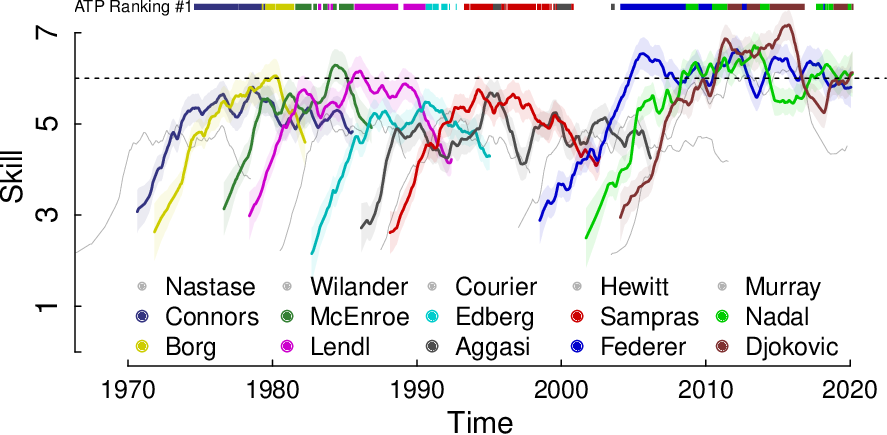
\includegraphics[page={1},width=.7\linewidth]{figures/atp}
    \caption{
    \en{Estimated learning curves of 8 famous players in ATP history.}
    \es{Estimación de las curvas de aprendizaje de 8 jugadores famosos de la historia de la ATP.}
    %
    \en{The shaded area represents an uncertainty equivalent to one standard deviation.}
    \es{El área sombrada representa una incertidumbre equivalente a un desvío estandar.}
    }
    
    \label{fig:atp}
\end{figure}
%
\en{The advantage of TrueSkill Through Time, over TrueSkill, is that by modeling the entire dynamic process it allows us to make comparisons of skills over time.}
\es{La ventaja de TrueSkill Through Time, respecto de TrueSkill, es que al modelar el proceso dinámico permite hacer comparaciones temporales de la habilidad.}
%
\en{It is interesting to see that the skill of tennis players did not increase so much over the years: on the contrary the players of the 1980s were more skilled than those of the 1990s, and reached a skill similar to what Federer, Nadal and Djokovic had in 2020.}
\es{Es interesante ver que la habilidad de los tenistas no aumentó tanto con los años: al contrario los jugadores de la década de los 80 fueron más habilidosos que aquellos de la década de los 90, y alcanzaron una habilidad similar a la que Federer, Nadal y Djokovic tuvieron en el año 2020.}
%
\en{Perhaps the most notable change introduced by professionalism is the stability of learning curves, which is seen in today's players as opposed to the early players.}
\es{Quizás el cambio más notable introducido por el profesionalismo sea la estabilidad de las curvas de aprendizaje, que se aprecia en los jugadores actuales a diferencia de los primeros jugadores.}














































































































%% -- Manuscript ---------------------------------------------------------------
%% - When describing longer chunks of code that are _not_ meant for execution
%%   (e.g., a function synopsis or list of arguments), the environment {Code}
%%   is recommended. Alternatively, a plain {verbatim} can also be used.
%%   (For executed code see the next section.)

\section{Models and software} 

\en{Probabilistic inference offers a generally applicable framework~\citep{Bishop2013} in which all the assumptions are made explicit through a generative model, and inference can always be solved by applying the sum and product rules over the joint distribution represented by the model.}
\es{La inferencia probabil\'istica ofrece un marco de aplicaci\'on general~\citep{Bishop2013} en el que todos los supuestos se hacen expl\'icitos a trav\'es de un modelo generativo y toda inferencia se hace aplicando las reglas de la suma y el producto sobre la distribuci\'on conjunta representada por el modelo.}
%
\en{In this section we will explain all the details of the probabilistic framework in the context of the TrueSkill Through Time problem.}
\es{En esta secci\'on explicaremos todos los detalles del marco probabil\'isitico en el contexto del problema TrueSkill Through Time.}
%
\en{In the section~\ref{sec:sumProductAlgorithm} we will introduce the \emph{sum-product algorithm}, which allows to efficiently apply the sum and product rules to compute the marginal distribution (e.g. the posterior and the prior predicition) from the joint distributions.}
\es{En la secci\'on~\ref{sec:sumProductAlgorithm} introduciremos el \emph{sum-product algorithm}, que permite aplicar eficientemente las reglas de la suma y el producto para computar distribuciones marginal (e.g. el posterior y la predicción a priori) a partir de la distribuci\'on conjunta.}
% %
% \en{In the section~\ref{sec:propiedades} we list the properties that we will need to derive the marginal distributions of interest.}
% \es{En la secci\'on~\ref{sec:propiedades} enumeramos las propiedades que necesitaremos para derivar las distribuciones marginales de inter\'es.}
% %
% \en{In the section \ref{sec:Gasussian} we introduce the implementation details of the class \texttt{Gaussian}.}
% \es{En las sección \ref{sec:Gasussian} introducimos los detalles de implementaci\'on de la clases \texttt{Gaussian}.}
% %
% \en{In the sections \ref{sec:2vs2}, \ref{sec:empate}, \ref{sec:approximate_posterior}, and \ref{sec:iterative_posterior} we show respectively how to solve the prior prediction and the exact posterior of an event, we introduce ties into the model, we explain how to approximate the posterior of a single event, and we give the general multi-team solution.}
% \es{En las secciones \ref{sec:2vs2}, \ref{sec:empate}, \ref{sec:approximate_posterior}, y \ref{sec:iterative_posterior} mostramos respectivamente c\'omo resolver la predicci\'on a priori y el posterior exacto de un evento, instroucimos la posibilidad de empates en el modelo, explicamos c\'omo aproximar el posterior, y damos la soluci\'on general multi-equipos.}
% %
% FALTA HISTORY
% %
% En la secci\'on~\ref{history} mostamos los pasos matem\'aticos requeridos para resolver el modelo TTT.
% %
% En la subsecci\'on~\ref{estructuras} introducimos las estructuras de datos utlizadas para generar la hsitoria.
% %
% En la subsecci\'on~\ref{trueskill} realizamos la inicializaci\'on de la historia, la que genera un resultado equivalente a trueskill.
% %
% En la subseci\'on~\ref{TTT} mostramos el algoritmo utilizado para converger las estmaciones.
% %
% 

\subsection{Sum-product algorithm} \label{sec:sumProductAlgorithm}

\en{The \emph{sum-product algorithm}~\citep{Kschischang2001} is a general procedure that takes advantage of the structure of the joint probability distribution imposed by the causal model to efficiently apply the rules of probability, the \ref{eq:sum_rule} and the \ref{eq:product_rule}.}
\es{El \emph{sum-product algorithm}~\citep{Kschischang2001} es un procedimiento general que aprovecha la estructura de la disstribuci\'on de probabilidad conjunta que impone el modelo causal para aplicar eficientemente las reglas de la probabilidad, la~\ref{eq:sum_rule} y la~\ref{eq:product_rule}.}
%
\en{Any model can be factored into the product of conditional probabilities.}
\es{Cualquier modelo puede factorizarse en el producto de probabilidades condicionales.}
%
\en{By making use of the independencies between variables (figure~\ref{fig:generative_model}) our model can be factored as,}
\es{Haciendo uso de las independencias entre las variables (figura~\ref{fig:generative_model}) nuestro modelo puede factorizarse como,}
%
\begin{equation} \label{eq:factorization}
 p(\bm{s},\bm{p},d,r) = p(s_1)p(s_2)p(p_1|s_1)p(p_2|s_2)p(d|\bm{p})P(r|d)
\end{equation}
%
\en{In figure~\ref{fig:factor_graph} we show this factorization graphically.}
\es{En la figura~\ref{fig:factor_graph} mostramos gr\'aficamente la factorizaci\'on.}
%
\en{These types of representations, known as \emph{factor graph}, are graphs with two types of nodes: variable nodes (white circles), and function nodes (black squares).}
\es{A este tipo de representaciones, conocidas como \emph{factor graph}, son gr\'afos con dos tipos de nodos: los nodos variables (círculos blancos), y los nodos funciones (cuadrados negros).}
%
\en{The edge between node variables and node functions represent the mathematical relationship ``the variable $v$ is an argument of the function $f$''.}
\es{Los ejes entre los nodos variables y los nodos funciones representan la relaci\'on matem\'atica ``la variable $v$ es argumento de la funci\'on $f$''.}
%
\begin{figure}[ht!]
\centering \small
    \tikz{         
%         \node[const, above=of fr] (nfr) {$f_r$}; %
% 	\node[const, above=of nfr] (dfr) {\large $\mathbb{I}(d >0)$}; %
    
    
    \node[factor] (fr) {} ; 
    %\node[const, left=of fr, xshift=-1.35cm] (r_name) {\small \en{Result}\es{Resultado}:}; 
    \node[const, left=of fr] (nfr) {\normalsize $P(r|d)$}; 
    \node[const, right=of fr] (dfr) {\normalsize \hspace{2.4cm} $P(r|d)=\mathbb{I}(d>0)$}; 

    \node[latent, above=of fr, yshift=-0.6cm] (d) {$d$} ; %
    \node[const, left=of d, xshift=-1.35cm] (d_name) {\small \en{Difference}\es{Diferencia}:};
    
    
    \node[factor, above=of d,yshift=-0.6cm] (fd) {} ; 
    \node[const, left=of fd] (nfd) {\normalsize $p(d|\bm{p})$}; 
    \node[const, right=of fd] (dfd) {\normalsize \hspace{2.4cm} $p(d|\bm{p}) =\delta(d=p_1-p_2) $}; 
    
    
    \node[latent, above=of fd, xshift=-0.8cm, yshift=-0.6cm] (p1) {$p_1$} ; %
    \node[latent, above=of fd, xshift=0.8cm, yshift=-0.6cm] (p2) {$p_2$} ; %
    \node[const, left=of p1, xshift=-0.55cm] (p_name) {\small \en{Performance}\es{Rendimiento}:}; 

    \node[factor, above=of p1 ,yshift=-0.6cm] (fp1) {} ; 
    \node[factor, above=of p2 ,yshift=-0.6cm] (fp2) {} ; 
    
    \node[latent, above=of fp1,yshift=-0.6cm] (s1) {$s_1$} ; %
    \node[latent, above=of fp2,yshift=-0.6cm] (s2) {$s_2$} ; %
    
    \node[factor, above=of s1 ,yshift=-0.6cm] (fs1) {} ; 
    \node[factor, above=of s2 ,yshift=-0.6cm] (fs2) {} ; 
    
    
    \node[const, left=of fp1] (nfp1) {\normalsize $p(p_1|s_1)$};
    \node[const, right=of fp2] (nfp2) {\normalsize $p(p_2|s_2)$};
    \node[const, right=of fp2] (dfp2) {\normalsize \hspace{1.6cm} $p(p_i|s_i)=\N(p_i|s_i,\beta^2)$};

    \node[const, left=of s1, xshift=-.85cm] (s_name) {\small \en{Skill}\es{Habilidad}:}; 
    
    \node[const, left=of fs1] (nfs1) {\normalsize $p(s_1)$};
    \node[const, right=of fs2] (nfs2) {\normalsize $p(s_2)$};
    \node[const, right=of fs2] (dfs) {\normalsize \hspace{1.6cm} $p(s_i) = \N(s_i|\mu_i,\sigma_i^2)$};

    
    \edge[-] {d} {fr};
    \edge[-] {p1,p2,d} {fd};
    \edge[-] {fp1} {p1,s1};
    \edge[-] {fp2} {p2,s2};
    \edge[-] {fs1} {s1};
    \edge[-] {fs2} {s2};
    %\node[invisible, right=of p2, xshift=4.35cm] (s-dist) {};
}
     \caption{
     \en{Graphical way of representing the factorization of joint distibution induced by the basic causal model (Eq.~\ref{eq:factorization}).}
     \es{Forma gráfica de representar la factorizaci\'on de la distribución conjunta inducida por el modelo causal básico (ecuación~\eqref{eq:factorization}).}
     %
     \en{Black squares represent the functions, white circles represent the variable, and the edges between them represent the mathematical relationship ``the variable is argument of the function''.}
     \es{Los cuadrados negros representan las funciones, los c\'irculos blancos representan las variable, y los ejes entre ellos representan la relaci\'on matem\'atica ``la variable es argumento de la funci\'on''.}
     %
     }
    \label{fig:factor_graph}
\label{modelo}
\end{figure} 
%
% \en{The structure encodes the minimum number of steps required to calculate any marginal probability distribution.}
% \es{La estructura codifica la m\'inima cantidad de pasos que se requieren para calcular cualquier distribuci\'on de probabilidad marginal.}
%
\en{In our case we want to compute two marginals, the proportional posterior of the skills $p(s_i, r)$ and the a prior probability of the result $p(r)$.}
\es{En nuestro caso querermos computar dos marginales, el posterior de las habilidades $p(s_i, r)$ y la probabilidad a priori del resultado $p(r)$.}
%
\en{The \emph{sum-product algorithm} is a general way of breaking down the rules of probability as messages that are sent locally between the nodes of the \emph{factor graph}.}
\es{El \emph{sum-product algorithm} es una forma general de descomponer las reglas de la probabilidad como mensajes que se env\'ian localmente los nodos del \emph{factor graph}.}
%
\en{There are two types of messages: the messages that variable nodes send to their functions neighbors ($m_{v \rightarrow f}(v)$); and the messages that function nodes send to their variable neighbors ($m_{f \rightarrow v}(v)$).}
\es{Hay dos tipos de mensajes: los mensajes que envian los nodos variables a sus funciones vecinas ($m_{v \rightarrow f}(v)$); y los mensajes que envian los nodos funciones a sus variables vecinas ($m_{f \rightarrow v}(v)$).}
%
\en{The messages sent by the variable nodes encode a portion of the product rule.}
\es{Los mensajes que env\'ian los nodos variables codifican una porci\'on de la regla del producto.}
%
\begin{equation*}\label{eq:m_v_f} \tag{\text{\en{product step}\es{paso productorial}}}
m_{v \rightarrow f}(v) = \prod_{h \in n(v) \setminus \{f\} } m_{h \rightarrow v}(v)
\end{equation*}
%
\en{Where $n(v)$ represents the set of node neighbors of $v$.}
\es{Donde $n(v)$ representa el conjunto de vecinos del nodo $v$.}
%
\en{In short, the messages sent by a $v$ variable is simply the product of the messages that $v$ received from the rest of their neighbors $h \in n(v)$ except $f$.}
\es{En pocas palabras, los mensajes que env\'ia una variables $v$ es simplemente la multiplicaci\'on de los mensajes que recibi\'o del resto de sus vecinos $h \in n(v)$ salvo $f$.}
%
\en{And the messages sent by the function nodes encode a portion of the sum rule.}
\es{Y los mensajes que env\'ian los nodos funciones codifican una parte de la regla de la suma.}
%
\begin{equation*}\label{eq:m_f_v}  \tag{\text{\en{sum step}\es{paso sumatorial}}}
m_{f \rightarrow v}(v) = \int \cdots \int \Big( f(\bm{h},v) \prod_{h \in n(f) \setminus \{v\} } m_{h \rightarrow f}(h) \Big) \,  d\bm{h}
\end{equation*}
%
\en{Where $\bm{h} = n(f)\setminus \{v\}$ is the set of all of neighbors of $f$ except $v$, and $f(\bm{h},v)$ represents the function $f$, evaluated in all its arguments.}
\es{Donde $\bm{h} = n(f)\setminus \{v\}$ es el conjunto de todos los vecinos de $f$ salvo $v$, y $f(\bm{h},v)$ represeta la funci\'on $f$, evaluada en todos sus argumentos.}
%
\en{In short, the messages sent by a function $f$ to a neighboring variable $v$ is simply the integration over $\bm{h}$ of the product of itself and all the messages that $f$ receives from the rest of its neighbors $\bm{h}$ except $v$.}
\es{En pocas palabras, los mensajes que enviado por una funci\'on $f$ a una variable vecina $v$ es simplemente la integraci\'on sobre $\bm{h}$ del producto de si mismo con todos los mensajes que $f$ recibe del resto de sus vecinos $\bm{h}$ salvo $v$.}
%
% \en{The composition of messages generates a partial computation.}
% \es{La composici\'on de mensajes va generando un computo parcial.}
% %
\en{Finally, the marginal probability distribution of a $v$ variable is simply the product of the messages that $v$ receives from its neighbors.}
\es{Finalmente, la distribuci\'on de probabilidad marginal de una variable $v$ es simplemente la multiplicaci\'on de los mensajes que $v$ recibe de sus vecinos.}
%
\begin{equation*}\label{eq:marginal}  \tag{\text{marginal}}
p(v) = \prod_{h \in n(v)} m_{h \rightarrow v}
\end{equation*}


\subsection{\en{Mathematical properties and notation}\es{Propiedades matem\'aticas y notaci\'on}}\label{sec:propiedades}

\en{The efficiency of TrueSkill Through Time is achieved because the marginals are computed analytically.}
\es{La eficiencia de TrueSkill Through Time se obtiene gracias que las marginales se computan de forma analítica.}
%
\en{In this section we list the properties that we will use to derive the exact and the approxiamte messages that arise from the sum-product algorithm.}
\es{En esta secci\'on enumeramos las propiedades que usaremos para derivar los mensajes exactos y aproximados que surgen del \emph{sum-product algorithm}.}
%
\en{Although these properties are widely known, we attach their full demonstrations in the supplemental material.}
\es{Aunque estas propiedades son ampliamente conocidas, adjuntamos sus demostraciones completas en material suplementario.}

% Parrafo

% \en{Let $\N$ be the Gaussian probability distribution, $\Phi$ the cumulative Gaussian distribution, $\mathbb{I}$ the indicator function.}
% \es{Sea $\N$ la ditribuci\'on de probabilidad gaussiana, $\Phi$ la acumulada de una distribuc\'on gaussiana, $\mathbb{I}$ la funci\'on indicadora.}
%
\en{The first property states that the product of two Gaussian distributions, both evaluated at the same point $x$, can be expressed as the product of two other Gaussian distributions, for which only one of them is evaluated at $x$.}
\es{La primera propiedad establece que el producto de dos distribuciones Gaussianas, ambas evaluadas en el mismo punto $x$, pueden expresarse como la producto de otras dos distribuciones Gaussianas, para las que sólo una de ellas está evaluada en $x$.}
%
\begin{equation*}\label{eq:gaussian_product} \tag{\text{\en{Gaussian product}\es{Producto de gaussianas}}}
\N(x|\mu_1,\sigma_1^2)\N(x|\mu_2,\sigma_2^2) \overset{\ref{multiplicacion_normales}}{=} \N(\mu_1|\mu_2,\sigma_1^2+\sigma_2^2) \N(x|\mu_{*},\sigma_{*}^2)
\end{equation*}
%
\en{where}\es{con} $\mu_{*} = \frac{\mu_1}{\sigma_1^2} + \frac{\mu_2}{\sigma_2^2}$ y $\sigma_{*}^2 = \left(\frac{1}{\sigma_1^2} + \frac{1}{\sigma_2^2} \right)^{-1}$.
%
\en{Something similar occurs with the division of two Gaussian distributions, both evaluated at the same point $x$.}
\es{Algo similar ocurre con la división de dos distribuciones Gaussianas, ambas evaluadas en el mismo punto $x$.}
\begin{equation*}\label{eq:gaussian_division} \tag{\text{\en{Gaussian division}\es{División de gaussianas}}}
\N(x|\mu_1,\sigma_1^2)/\N(x|\mu_2,\sigma_2^2) \overset{\ref{sec:division_normales}}{\propto} \N(x|\mu_{\div},\sigma_{\div}^2)/\N(\mu_1|\mu_2,\sigma_1^2+\sigma_2^2) 
\end{equation*}
%
\en{where}\es{con} $\mu_{\div} = \frac{\mu_1}{\sigma_1^2} - \frac{\mu_2}{\sigma_2^2}$ y $\sigma_{\div}^2 = \left(\frac{1}{\sigma_1^2} - \frac{1}{\sigma_2^2} \right)^{-1}$ .
%
\en{The indicator function $\mathbb{I}(\cdot=\cdot)$ is worth $1$ when equality is true and $0$ otherwise.}
\es{La funci\'on indicadora $\mathbb{I}(\cdot=\cdot)$ vale $1$ cuando la igualdad es verdadera y $0$ en caso contrario.}
%
% \en{When we can use it to replace variable within an integral,}
% \es{Cuando podemos usarla para remplazar variable dentro de una integral,}
% %
% \begin{equation}\label{eq:integral_con_indicadora} \tag{\text{\en{Indicator function}\es{Función indicadora}}}
% \begin{split}
%  \iint  \mathbb{I}(x=h(y,z)) f(x) g(y)\, dx\, dy = \int f(h(y,z)) g(y) dy
%  \end{split}
% \end{equation}
% %
% \en{the dimensionality of the problem is reduced.}
% \es{la dimensionalidad del problema se reduce.}
% %
\en{The indicator function is used to represent probability distributions of non-random discrete variables, as the result of the games given the difference of performances $p(r|d)$.}
\es{La función indicadora se usa para representar distribuciones de probabilidad de variables discretas no aleatoria, como el resultado de los juegos dada la diferencia de rendimientos $p(r|d)$}
%
\en{Similarly, the dirac delta function, $\delta(\cdot=\cdot)$, which is used to represent probability distributions of non-random continuous variables, such as the difference of performances given the agents' performances $p(d|\bm{p})$.}
\es{De la misma forma, la función delta de dirac, $\delta(\cdot=\cdot)$, que se usa para representar distribuciones de probabilidad de variables continuas no aleatoria como la diferencia de rendimiento dados rendimientos $p(d|\bm{p})$.}
%
\en{When we can use it to replace variable within an integral,}
\es{Cuando podemos usarla para remplazar variable dentro de una integral,}
%
\begin{equation*}\label{eq:integral_con_dirac} \tag{\text{\en{Dirac delta function}\es{Función delta de dirac}}}
\begin{split}
 \iint  \delta(x=h(y,z)) f(x) g(y)\, dx\, dy = \int f(h(y,z)) g(y) dy
 \end{split}
\end{equation*}
\en{the dimensionality of the problem is reduced.}
\es{la dimensionalidad del problema se reduce.}
%
\en{We will also use the properties derived from the symmetry of Gaussians.}
\es{Usaremos además las propiedades que se derivan de la simetría de Gaussianas.}
\begin{equation*}\label{eq:simetria} \tag{\text{\en{Gaussian symmentry}\es{Simetría de gaussianas}}}
 \N(x|\mu,\sigma^2) = \N(\mu|x,\sigma^2) = \N(-\mu|-x,\sigma^2) = \N(-x|-\mu,\sigma^2) 
\end{equation*}
%
\en{The Gaussian standardization,}
\es{La estandizarización de la Gaussiana,}
\begin{equation*}\label{eq:estandarizar} \tag{\text{\en{Gaussian standarization}\es{Estandarización de gaussianas}}}
  \N(x|\mu,\sigma^2) = \N((x-\mu)/\sigma | 0, 1)
\end{equation*}
%
\en{Equality between the Gaussian distribution and the derivative of their cumulative distribution,}
\es{La igualdad entre la distribución Gaussiana y la derivada de la acumulada,}
\begin{equation*}\label{eq:phi_norm} \tag{\text{\en{Derivative of the cumulative Gaussian}\es{Derivada de la gaussiana acumulada}}}
 \frac{\partial}{\partial x} \Phi(x|\mu,\sigma^2) = \N(x|\mu,\sigma^2)
\end{equation*}
%
\en{which is valid by definition.}
\es{que vale por definición.}
%
\en{The symmetry of the cumulative Gaussian distribution.}
\es{La simetría de la distribución Gaussiana acumulada.}
\begin{equation*}\label{eq:phi_simetria} \tag{\text{\en{Symmetry of the cumulative Gaussian}\es{Simetría de la gaussiana acumulada}}}
\Phi(0|\mu,\sigma^2) = 1-\Phi(0|-\mu,\sigma^2)
\end{equation*}

\subsection{Gaussian}\label{sec:Gasussian}

\en{The \texttt{Gaussian} class does most of the computation of the packages.}
\es{La clase \texttt{Gaussian} realiza la mayor parte del c\'omputo en todos los paquetes.}
%
\en{It is represented by two parameters, the mean (\texttt{mu}) and the standard deviation (\texttt{sigma}).}
\es{Se representa mediante dos par\'ametros, la media y el desv\'io estandar.}
% %
\begin{lstlisting}[backgroundcolor=\color{all},label=lst:N1_N2, caption={\en{Initialization of Gaussians distributions}\es{Inicialización de distirbuciones gaussianas}}, belowskip=-1.0 \baselineskip, aboveskip=-0 \baselineskip]
\end{lstlisting}
\begin{lstlisting}[backgroundcolor=\color{all}, belowskip=0.0 \baselineskip]
N1 = Gaussian(mu = 1.0, sigma = 1.0); N2 = Gaussian(1.0, 2.0)  
\end{lstlisting}
%
\en{The class overwrites the operators addition (\texttt{+}), subtraction (\texttt{-}), product (\texttt{*}) and division (\texttt{/}) with the main properties required to compute the marginal distributions in the TrueSkill Through Time model.}
\es{La clase sobreescribe los operadores suma (\texttt{+}), resta (\texttt{-}), producto (\texttt{*}) y divisi\'on (\texttt{/}) con las principales propiedades requeridas para computar las distribuciones marginales en el modelo TrueSkill Through Time.}
%
\begin{equation*} \tag{\texttt{N1 * N2}}
 \N(x|\mu_1,\sigma_1^2)\N(x|\mu_2,\sigma_2^2) \overset{\ref{multiplicacion_normales}}{\propto} \N(x|\mu_{*},\sigma_{*}^2)
\end{equation*}
%
\begin{equation*} \tag{\texttt{N1 / N2}}
 \N(x|\mu_1,\sigma_1^2)/\N(x|\mu_2,\sigma_2^2)  \overset{\ref{sec:division_normales}}{\propto} \N(x|\mu_{\div},\sigma_{\div}^2)
\end{equation*} 
%
\vspace{-0.3cm}
%
\begin{equation*} \tag{\texttt{N1 + N2}} \label{eq:suma_normales}
\begin{split}
\iint \delta(t=x + y) \N(x|\mu_1, \sigma_1^2)\N(y|\mu_2, \sigma_2^2) dxdy \overset{\text{\ref{suma_normales_induccion}}}{=} \N(t|\mu_1+\mu_2,\sigma_1^2 + \sigma_2^2)
\end{split}
\end{equation*}
%
\vspace{-0.5cm}
%
\begin{equation*} \tag{\texttt{N1 - N2}} \label{eq:resta_normales}
\begin{split}
\iint \delta(t = x - y) \N(x|\mu_1, \sigma_1^2)\N(y|\mu_2, \sigma_2^2) dxdy \overset{\text{\ref{suma_normales_induccion}}}{=} \N(t|\mu_1 - \mu_2,\sigma_1^2 + \sigma_2^2)
\end{split}
\end{equation*}

\subsection{\en{The exact solution of the team model}\es{La solución exacta del modelo de equipos}}\label{sec:2vs2}

\en{TrueSkill allows to estimate the skill of individuals even when they play in teams.}
\es{TrueSkill permite estimar la habilidad de los individuos incluso cuando estos juegan en equipo.}
%
\en{The model assumes that the team with the highest performance wins, $r = (t_i > t_j)$, where $t_i$ and $t_j$ represent the team performances.}
\es{El modelo supone que gana el equipo con mayor rendimiento, $r = (t_i > t_j)$, donde $t_i$ y $t_j$ representan los desempeños de los equipos.}
%
\en{In figure~\ref{fig:modelo_trueskill_2vs2} we show the factor graph.}
\es{En la figura~\ref{fig:modelo_trueskill_2vs2} mostramos la factorizaci\'on gr\'afica.} 
%
\begin{figure}[ht!]
  \centering
  \scalebox{.9}{
  \tikz{
      
        \node[factor] (fr) {} ;
        \node[const, right=of fr] (nfr) {$f_{r}$}; %
	
	\node[latent, above=of fr, yshift=-0.4cm] (d) {$d$} ; %
        \node[factor, above=of d, yshift=-0.4cm] (fd) {} ;
        \node[const, above=of fd] (nfd) {$f_{d}$}; %
	
        
        \node[latent, left=of fd,xshift=0.4cm] (ta) {$t_a$} ; %
        \node[factor, left=of ta,xshift=0.4cm] (fta) {} ;
        \node[const, above=of fta] (nfta) {$f_{t_a}$}; %
        
        \node[latent, left=of fta,yshift=1cm,xshift=0.4cm] (p1) {$p_1$} ; %
        \node[factor, left=of p1,xshift=0.4cm] (fp1) {} ;
        \node[const, above=of fp1] (nfp1) {$f_{p_1}$}; %
        
        \node[latent, left=of fp1,xshift=0.4cm] (s1) {$s_1$} ; %
        \node[factor, left=of s1,xshift=0.4cm] (fs1) {} ;
	\node[const, above=of fs1] (nfs1) {$f_{s_1}$}; %
     
        \node[latent, left=of fta,yshift=-1cm,xshift=0.4cm] (p2) {$p_2$} ; %
        \node[factor, left=of p2,xshift=0.4cm] (fp2) {} ;
        \node[const, above=of fp2] (nfp2) {$f_{p_2}$}; %
        
        \node[latent, left=of fp2,xshift=0.4cm] (s2) {$s_2$} ; %
        \node[factor, left=of s2,xshift=0.4cm] (fs2) {} ;
	\node[const, above=of fs2] (nfs2) {$f_{s_2}$}; %
        
            
        \node[latent, right=of fd,xshift=-0.4cm] (tb) {$t_b$} ; %
        \node[factor, right=of tb,xshift=-0.4cm] (ftb) {} ;
        \node[const, above=of ftb] (nftb) {$f_{t_b}$}; %
        
        \node[latent, right=of ftb,yshift=1cm,xshift=-0.4cm] (p3) {$p_3$} ; %
        \node[factor, right=of p3,xshift=-0.4cm] (fp3) {} ;
        \node[const, above=of fp3] (nfp3) {$f_{p_3}$}; %
        
        \node[latent, right=of fp3,xshift=-0.4cm] (s3) {$s_3$} ; %
        \node[factor, right=of s3,xshift=-0.4cm] (fs3) {} ;
	\node[const, above=of fs3] (nfs3) {$f_{s_3}$}; %
     
        \node[latent, right=of ftb,yshift=-1cm,xshift=-0.5cm] (p4) {$p_4$} ; %
        \node[factor, right=of p4,xshift=-0.4cm] (fp4) {} ;
        \node[const, above=of fp4] (nfp4) {$f_{p_4}$}; %
        
        \node[latent, right=of fp4,xshift=-0.4cm] (s4) {$s_4$} ; %
        \node[factor, right=of s4,xshift=-0.4cm] (fs4) {} ;
	\node[const, above=of fs4] (nfs4) {$f_{s_4}$}; %
     
        \edge[-] {fr} {d};
	\edge[-] {d} {fd};
	
        \edge[-] {fd} {ta};
        \edge[-] {ta} {fta};
        \edge[-] {fta} {p1};
        \edge[-] {p1} {fp1};
        \edge[-] {fp1} {s1};
        \edge[-] {s1} {fs1};
        \edge[-] {fta} {p2};
        \edge[-] {p2} {fp2};
        \edge[-] {fp2} {s2};
        \edge[-] {s2} {fs2};
        	
	\edge[-] {fd} {tb};
        \edge[-] {tb} {ftb};
        \edge[-] {ftb} {p3};
        \edge[-] {p3} {fp3};
        \edge[-] {fp3} {s3};
        \edge[-] {s3} {fs3};
        \edge[-] {ftb} {p4};
        \edge[-] {p4} {fp4};
        \edge[-] {fp4} {s4};
        \edge[-] {s4} {fs4};
        
	
	\node[const, below=of fr,xshift=7cm,yshift=-0.3cm] (dfr) { $f_r = \mathbb{I}(d>0)$}; %
	\node[const, left=of dfr,xshift=-0.5cm] (dfd) {$f_d = \delta(d=t_a - t_b)$}; %
	\node[const, left=of dfd,xshift=-0.5cm] (dft) {$f_{t_e} = \delta(t_e = \sum_{i \in A_e} p_i)$}; %
        \node[const, left=of dft,xshift=-0.5cm] (dfp) {$f_{p_i} = \N(p_i|s_i,\beta^2)$}; %
        \node[const, left=of dfp,xshift=-0.5cm] (dfs) {$f_{s_i} = \N(s_i|\mu_i,\sigma^2)$}; %
   }
   }
  \caption{
  \en{Factor graph of a 2 vs 2 game.}
  \es{Factorizaci\'on gr\'afica de una partida 2 vs 2.}
  %
  \en{We incorporated a new variable, $t$, that models the team performance.}
  \es{Incorporamos una variable nueva, $t$, que modela el desempeño de los equipos.}
  }
  \label{fig:modelo_trueskill_2vs2}
\end{figure}
%
\en{In Figure~\ref{fig:modelo_trueskill_2vs2}, team performance is modeled as the sum of the individual performances of its members.}
\es{En la figura~\ref{fig:modelo_trueskill_2vs2}, el desempeño de los equipos se modela como una suma de los desempeños de sus integrantes.}
%
\en{Every game with two teams has an analytical solution.}
\es{Toda partida con dos equipos tiene soluci\'on analítica.}

% Parrafo

\en{In this section we will show the steps to compute the exact evidence and the exact likelihoods of a game with two teams of two players.}
\es{En esta secci\'on vamos a mostrar los pasos para calcular la evidencia exacta y los likelihoods exactos de una partida con dos equipos de dos jugadores.}
%
\en{We only need the \emph{sum-product algorithm} and the properties mentioned above.}
\es{Sólo necesitamos el \emph{sum-product algorithm} y las propiedades arriba mencionadas.}
%
\en{We will start first with the ``descending'' messages, from the priors to the result until compute the evidence, and then we will continue with the ``ascending'' messages, from the observed result and to the priors until compute the posterior of each agent.}
\es{Empezaremos primero con los mensajes ``descendentes'', desde los priors a el resultado hasta calcular la evidencia, y seguiremos con los mensajes ``ascendentes'', desde el resultado observado a los priors hasta calcular el posterior de cada agente.}

\paragraph{\en{Descending messages}\es{Mensajes descendentes}.}

\en{Following the \ref*{eq:m_f_v} of the sum-product algorithm and the factorization of the model displayed at Figure~\ref{fig:modelo_trueskill_2vs2}, the messages from the skill factors $f_{s_i}$ to their variable $s_i$ are just the priors.}
\es{Siguiendo el~\ref*{eq:m_f_v} del \emph{sum-product algorithm} y la factorizaci\'on del modelo presentado en la figura~\ref{fig:modelo_trueskill_2vs2}, los mensajes de los factores de habilidad $f_{s_i}$ a su variable $s_i$ no son otra cosa m\'as que el priors.}
%
\begin{equation*}\label{eq:m_fs_s} \tag{\texttt{prior}}
 m_{f_{s_i} \rightarrow s_i}(s_i) = \N(s_i| \mu_i, \sigma_i^2)
\end{equation*}
%
\en{We have access to this message by calling the \texttt{prior} attribute of the initialized \texttt{a} agent, \texttt{a.prior}.}
\es{Tenemos acceso a este mensaje llamando al atributo \texttt{prior} de los jugadores \texttt{a} que se tengan inicializados, \texttt{a.prior}.}
%
\en{The next message, the one that the variable $s_i$ sends to the performance factor $f_{p_i}$ is also the prior, in this case due to the~\ref*{eq:m_v_f} of the sum-product algorithm and the factorization of the model.}
\es{El siguiente mensaje, el que la variable $s_i$ le env\'ia al factor rendimiento $f_{p_i}$ tambi\'en es el prior, en este caso debido al~\ref*{eq:m_v_f} del \emph{sum-product algorithm} y la factorizacion del modelo.}
%
\en{Since it is trivial to calculate the messages sent by the variables (they are always the product of the messages they receive from behind), we will avoid writing them.}
\es{Debido a que es trivial calcular los mensajes que envian las variables (siempre es el producto de los mensajes que reciben de atrás), vamos a evitar escribirlos.}
%
\en{Let's see then the message that the performance factors $f_{p_i}$ send to their variable $p_i$.}
\es{Veamos entonces el mensaje que env\'ian los factores rendimiento $f_{p_i}$ a su variable $p_i$.}
%
\begin{equation*}\label{eq:m_fp_p} \tag{\texttt{performance()}}
m_{f_{p_i} \rightarrow p_i}(p_i) = \int \N(p_i| s_i, \beta^2) \N(s_i| \mu_i, \sigma_i^2) ds_i = \N(p_i|\mu_i,\beta^2 + \sigma_i^2)
\end{equation*}
%
\en{We have access to these messages through the \texttt{performance()} method of the \texttt{Player} class.}
\es{Tenemos acceso a estos mensajes mediante el método \texttt{performance()} de la clase \texttt{Player}.}
%
\begin{lstlisting}[backgroundcolor=\color{white},label=lst:performance, caption={\en{Computing the individual prior performance}\es{Computando el desempeño individual a priori}}, belowskip=-1.0 \baselineskip, aboveskip=0.0 \baselineskip]
\end{lstlisting}
\begin{paracol}{3}
\begin{lstlisting}[backgroundcolor=\color{julia}]
p1 = performance(a1)
p2 = performance(a2)
p3 = performance(a3)
p4 = performance(a4)
\end{lstlisting}
  \switchcolumn
\begin{lstlisting}[backgroundcolor=\color{python}]
p1 = a1.performance()
p2 = a2.performance()
p3 = a3.performance()
p4 = a4.performance()
\end{lstlisting}
   \switchcolumn
\begin{lstlisting}[backgroundcolor=\color{r}]
p1 = a1.performance()
p2 = a2.performance()
p3 = a3.performance()
p4 = a4.performance()
\end{lstlisting}  
\end{paracol}
%
\en{Where the agents \texttt{a1}, \texttt{a2}, \texttt{a3}, and \texttt{a4} were initialized at code~\ref{lst:player}.}
\es{Donde los agentes \texttt{a1}, \texttt{a2}, \texttt{a3} y \texttt{a4}, fueron inicializados en el código~\ref{lst:player}.}
%
\en{The message sent by the team factors $f_{t_e}$ to the team variable $t_e$ is an integral over all the individual performance variables, with the sum being equal to a constant $t_e$ (constraint imposed by the Dirac delta function).}
\es{El mensaje que envían los factores equipos $f_{t_e}$ a la variable equipo $t_e$ es una integral sobre todas las variables de rendimiento individuales, siendo la suma igual a una constante $t_e$ (restricción impuesta por la función delta de Dirac).}
%
\begin{equation*} \label{eq:m_ft_t} \tag{\texttt{ta = p1 + p2}}
\begin{split}
 m_{f_{t_e} \rightarrow t_e}(t_e) &= \iint \delta(t_e = p_i + p_j) \N(p_i|\mu_i,\beta^2 + \sigma_i^2)\N(p_j|\mu_j,\beta^2 + \sigma_j^2) dp_idp_j  \\ &=  \N(t_e|\underbrace{\mu_i+\mu_j}_{\text{\normalsize $\mu_e\phantom{^2}$}}, \underbrace{2\beta^2 + \sigma_i^2 + \sigma_j^2}_{\text{\normalsize $\sigma_e^2$}})
\end{split}
\end{equation*}
%
\en{The prior performance of the teams is a Gaussian distribution centered on the sum of the mean estimates $\mu_e = \mu_i + \mu_j$ with a variance $\sigma_e^2$ that includes both the uncertainties of the estimates, $\sigma_i^2 + \sigma_j^2$, and the variance of the individual performances, $\beta^2 + \beta^2$.}
\es{El desempeño a priori de los equipos es una distribución Gaussiana centrada en la suma de las estimaciones medias $\mu_e = \mu_i + \mu_j$ con una varianza que incluye tanto las incertidumbres de las estimaciones, $\sigma_i^2 + \sigma_j^2$, como la varianza de los rendimientos individuales, $\beta^2 + \beta^2$.}
%
\en{We have access to this message when we use the operator \texttt{+} of the class \texttt{Gaussian} to sum the agents' performances,}
\es{Tenemos acceso a este mensaje cuando usamos el operador \texttt{+} de la clase \texttt{Gaussian} para sumar los desempeños de los agentes,}
%
\begin{lstlisting}[backgroundcolor=\color{white},label=lst:team_performance, caption={\en{Computing the team prior performance}\es{Computando el desempeño a priori de los equipos}}, belowskip=-1.0 \baselineskip, aboveskip=0.0 \baselineskip]
\end{lstlisting}
\begin{lstlisting}[backgroundcolor=\color{all}]
ta = p1 + p2; tb = p3 + p4
\end{lstlisting}
%
\en{The next message, sent by the difference factor $f_{d_1}$ to the difference variable $d_1$ is,}
\es{El siguiente mensaje, que env\'ia el factor diferencia $f_{d_1}$ a la variable diferencia $d_1$ es,}
\begin{equation*}\label{eq:m_fd_d} \tag{\texttt{d = ta - tb}}
 \begin{split} 
  m_{f_{d} \rightarrow d}(d) & = \iint \delta(d = t_a - t_b) \N(t_a| \mu_a, \sigma_a^2)  \N(t_b| \mu_b, \sigma_b^2)  dt_adt_b \\[0.25cm]
  & = \N\big( d | \underbrace{\mu_a - \mu_b}_{\hfrac{\text{\en{Expected}\es{Differencia}}}{\text{\en{difference}\es{esperada}}}:  \ \psi}, \underbrace{\sigma_a^2 +\sigma_b^2}_{\hfrac{\text{\en{Total}\es{incertidumbre}}}{\text{\en{uncertainty}\es{total}}} : \ \vartheta^2}  \big) = \N(d | \psi, \, \vartheta^2)
 \end{split}
\end{equation*}
%
\en{The prior difference of performance is a Gaussian distribution centered on the a priori expected difference between teams $\psi = \mu_a - \mu_b$ with variance $\vartheta^2 = \sigma_a^2 + \sigma_b^2$ that includes the uncertainty of both teams.}
\es{La diferencia de desempeños a priori es una distribución gaussiana centrada en la diferencia esperada a priori $\psi = \mu_a - \mu_b$ con una varianza $\vartheta^2 = \sigma_a^2 + \sigma_b^2$ que incluye la incertidumbre de ambos equipos.}
%
\en{We have access to this message using the operator \texttt{-} of the class \texttt{Gaussian} to get de difference of teams' performances, \texttt{d = ta - tb}.}
\es{Tenemos acceso a este mensaje cuando usamos el operador \texttt{-} de la clase \texttt{Gaussian} para la diferencia de los desempeños de los equipos, \texttt{d = ta - tb}.}
%
\begin{lstlisting}[backgroundcolor=\color{white},label=lst:difference_performance, caption={\en{Computing the prior difference of performances}\es{Computando la diferencia de desempeños a priori}}, belowskip=-1.0 \baselineskip, aboveskip=0.0 \baselineskip]
\end{lstlisting}
\begin{lstlisting}[backgroundcolor=\color{all}]
d = ta - tb 
\end{lstlisting}
%
\en{The last descending message, sent by the factor $f_r$ to the variable $r$, is}
\es{El último mensaje descendente, el que envía el factor $f_r$ a la variable $r$, permite computar la evidencia, es decir la predicción a priori del resultado observado}
%
\begin{equation*}\label{eq:m_fr_r} \tag{\texttt{evidence}}
\begin{split}
 m_{f_{r} \rightarrow r}(r) = \int \mathbb{I}(d > 0) \N(d | \psi, \vartheta^2)  dd = 1 - \Phi(0|\psi, \vartheta^2)
\end{split}
\end{equation*}
%
\en{We have access to the prior probability of the observed result (or evidence) by computing the cumulative value from $0$ to $\infty$ of the team difference of performances distribution.}
\es{Tenemos acceso a la probabilidad a priori del resultado observado (o evidencia) calculando el valor acumulado desde $0$ hasta $\infty$ de la distribución de diferencia de desempeños de los equipos.}
%
\begin{lstlisting}[backgroundcolor=\color{white},label=lst:difference, caption={\en{Computing the prior prediction of the oberved result (or evidence)}\es{Computando la predicción a priori del resultado observado (o evidencia)}}, belowskip=-1.0 \baselineskip, aboveskip=0.0 \baselineskip]
\end{lstlisting}
\begin{paracol}{3}
\begin{lstlisting}[backgroundcolor=\color{julia}]
e = 1.0 - cdf(d, 0.0)
\end{lstlisting}  
 \switchcolumn
\begin{lstlisting}[backgroundcolor=\color{python}]
e = 1 - cdf(0,d.mu,d.sigma) 
\end{lstlisting} 
 \switchcolumn
\begin{lstlisting}[backgroundcolor=\color{r}]
e = 1 - cdf(0,d$mu,d$sigma) 
\end{lstlisting}   
\end{paracol}
%
\en{Where \texttt{e} contains the value of \texttt{evidence}.}
\es{Donde \texttt{e} contiene el valor de \texttt{evidence}.}


\paragraph{\en{Ascending messages}\es{Mensajes ascendentes}.}
%
\en{Let us now examine the ascending messages.}
\es{Examinemos ahora los mensajes ascendentes.}
%
\en{Just as downward messages could be interpreted as priors, in this case the upward messages can also be interpreted as likelihoods, because they transmit the information of the observed result.}
\es{Así como los mensajes descendente podíamos interpretarlos como priors, en este caso los mensajes ascendentes van a poder ser interprestados como likelihoods, debido a que transmiten la información del resultado observado.}
%
\en{The first ascending message is sent by the result factor $f_r$ to the difference variable $d$.}
\es{El primer mensaje ascendentes lo envía el factor de resultados $f_r$ a la variable de diferencia $d$.}
%
\begin{equation}%\label{eq:m_fr_d} \tag{\texttt{exact\_lhood\_d}}
\begin{split}
m_{f_r \rightarrow d}(d) & = \mathbb{I}(d>0)
\end{split}
\end{equation}
%
\en{The message contains just the indicator function of the factor $f_r$.}
\es{El mensaje sólo contiene la función indicadora propia del factor $f_r$.}
%
% \en{The ascending messages will not be computed step by step, we will give the code at the end.}
% \es{Los mensajes ascendentes no los vamos a ir computando paso a paso, daremos el código al final.}
%
\en{The message sent by difference factor $f_d$ to the winning team performance variables $t_e$ is,}
\es{El mensaje que el factor diferencia $f_d$ envía la variables de desempeño del equipo ganador $t_a$ es,}
\begin{equation}%\label{eq:m_fd_ta} \tag{\texttt{exact\_lhood\_ta}}
\begin{split}
m_{f_{d} \rightarrow t_a}(t_a) & = \iint \delta(d = t_a - t_b) \mathbb{I}(d > 0) \N(t_b | \mu_b , \sigma_b^2 ) \, dd\,dt_b \\
& = \int \mathbb{I}( t_a > t_b)  \N(t_b | \mu_b , \sigma_b^2 ) \,dt_b  \\
& = 1 - \Phi (0| t_a -\mu_b, \sigma_b^2) = \Phi (t_a| \mu_b, \sigma_b^2)
\end{split}
\end{equation}
%
\en{In this case, the previous upstream message is integrated with the downstream message from the other team.}
\es{En este caso se integra el mensaje ascendente anterior junto con el mensaje descendente del otro equipo.}
%
\en{This message, parametrized at $t_a$, is the cumulative of the Gaussian distribution of the opposing team's performances from $t_a$ to $\infty$, and encodes the likelihood of the winning team performance hypotheses.}
\es{Este mensaje, paramtrizado en $t_a$, es la acumulada de la distribución gaussiana de los rendimientos del equipo contrario desde $t_a$ hasta $\infty$, y codifica la verosimilitud de las hipótesis de rendimiento de equipo ganador.}
%
\en{The message sent by team performance factor $f_{t_a}$ to the variable of the individual performance $p_1$ is,}
\es{El mensaje enviado por el factor de rendimiento del equipo $f_{t_a}$ a la variable del rendimiento individual $p_1$ es,}
%
\begin{equation}%\label{eq:m_fta_p_inicial} \tag{\texttt{exact\_lhood\_p1}}
\begin{split}
m_{f_{t_a} \rightarrow p_1}(p_1)  & = \iint \delta( t_a = p_1 + p_2) \, N(p_2| \mu_2, \beta^2 + \sigma_2^2 ) \, \Phi (t_a| \mu_b , \sigma_b^2 ) \, dt_a dp_2 \\
& = \int  \, \N(p_2| \mu_2, \beta^2 + \sigma_2^2 ) \, \Phi (p_1 + p_2| \mu_b , \sigma_b^2 ) \, dp_2 \\
& = 1 - \Phi( 0 | p_1 + \underbrace{\mu_2 - \mu_b}_{\mu_1 - \psi}, \underbrace{\beta^2 + \sigma_2^2 + \sigma_b^2}_{\vartheta^2 - (\sigma_1^2 + \beta^2)}) \\
\end{split}
\end{equation}
%
\en{Again, the previous upstream message is integrated with a downstream message, the prior performance of their teammate.}
\es{Otra vez, el mensaje ascendente anterior se integra junto con un mensaje descendente, el desempeño a priori de su compañero de equipos.}
%
\en{The message, parameterized at $p1$, encodes the likelihood of the individual performance hypotheses of the winning player.}
\es{El mensaje, parametrizado en $p1$, codifica la verosimilitud de las hipótesis de rendimiento individual del jugador ganador.}
%
\en{The last message, sent by indivudal performance factor $f_{p_1}$ to the skill variable $s_1$ is,}
\es{El mensaje enviado por el factor de rendimiento individual $f_{p_1}$ a la variable del hbilidad $s_1$ es,}
%
\begin{equation}%\label{eq:m_fp_s1} \tag{\texttt{exact\_lhood\_s1}}
\begin{split}
m_{f_{p_1} \rightarrow s_1}(s_1) & = \int N(p_1| s_1, \beta^2) \, \Phi(p_1| \mu_1-\psi, \vartheta^2 - (\sigma_1^2 + \beta^2)) \, dp_1 \\[0.1cm]
& = 1 - \Phi(0 | \underbrace{(s_1 + \mu_2) - (\mu_3 + \mu_4)}_{\hfrac{\text{\en{Expected difference}\es{Diferencia esperada}}}{\text{\en{parameterized in }\es{parametrizada en }$s_1$}} } \ , \underbrace{\ \ \ \ \vartheta^2 - \sigma_1^2 \ \ \ \ }_{\hfrac{\text{\en{Total uncertainty}\es{Incertidumbre total}}}{\text{\en{except the one of }\es{salvo la de }$s_1$}}})\end{split}
\end{equation}
%
\en{This is the exact likelihood, and computes the prior probability of winning result if the player's true skill was $s_1$.}
\es{Este es el likelihood exacto, y computa la probabilidad a priori de un resultado ganador si la verdadera habilidad del jugador fuera $s_1$.}
%
\en{By assuming that the skill is known, we replace the average estimate $\mu_1$ by the hypothesis $s_1$ in the expected difference $\psi$, and remove its own uncertainty from the total uncertainty $\vartheta^2$.}
\es{Al suponer conocida la habilidad, remplazamos su estimaci\'on media $\mu_1$ por la hip\'otesis $s_1$ en la diferencia esperada $\psi$, y eliminamos su incertidumbre de la incertidumbre total $\vartheta^2$.}
%
% \begin{lstlisting}[backgroundcolor=\color{white},label=lst:delta_1, caption=\relax, belowskip=-1.0 \baselineskip, aboveskip=-0 \baselineskip]
% \end{lstlisting}
% \begin{paracol}{3}
% \begin{lstlisting}[backgroundcolor=\color{julia}]
% theta1 = d.sigma^2-a1.sigma^2
% theta1 = sqrt(theta1)
% function exact_lhood_s1(s)
%   psi1 = d.mu - a1.mu + s
%   N= Gaussian(psi1,theta1)
%   return 1-cdf(N,0.0)
% end
% \end{lstlisting}  
%  \switchcolumn
% \begin{lstlisting}[backgroundcolor=\color{python}]
% theta1 = theta**2 - sigma1**2
% theta1 = sqrt(theta1)
% def exact_lhood_s1(s):
%     delta1 = delta - mu1 + s1 
%     res=1-cdf(0,delta1,theta1)
%     return res
%     
% \end{lstlisting} 
%  \switchcolumn
% \begin{lstlisting}[backgroundcolor=\color{r}]
% theta1 = theta^2 - sigma1^2
% theta1 = sqrt(theta1)
% exact_lhood_s1 =function(s){
%   delta1 = delta - mu1 + s 
%   res=1-cdf(0,delta1,theta1)
%   return(res)
% }
% \end{lstlisting}   
% \end{paracol}

\subsection{\en{A Basic Draw Model}\es{Modelo b\'asico de empates}} \label{sec:empate}

\en{The draw model assumes that a tie occur when the difference in performance does not exceed a certain margin, $|t_a > t_b| \leq \varepsilon$.}
\es{El modelo supone que ocurre un empate cuando la diferencia de rendimientos no supera un cierto margen, $|t_a > t_b| \leq \varepsilon$.}
%
\en{In the figure~\ref{fig:draw_a} we display in graphical terms the probabilities of the three possible outcomes.}
\es{En la figura~\ref{fig:draw_a} se puede ver en t\'erminos gr\'aficos las probabilidades de los tres resultados posibles.}
%
\begin{figure}[ht!]
\centering
\begin{subfigure}[t]{0.48\textwidth}
 \includegraphics[width=1\textwidth]{figures/draw.pdf} 
 \caption{
 \en{The three possible results}
 \es{Los tres posibles resultados}
 }
 \label{fig:draw_a}
\end{subfigure}
\begin{subfigure}[t]{0.48\textwidth}
  \includegraphics[page=2,width=1\textwidth]{figures/draw.pdf}
  \caption{
  \en{Constant draw probability}
  \es{Probabilidad de empate constante}
  }
 \label{fig:draw_b}
\end{subfigure}
  \caption{
  \en{Distribution of performance difference under the draw model.}
  \es{Distribución de diferencia de desempeño bajo el modelo de empate.}
  %
  \en{In Figure~\ref{fig:draw_a} we show an example of the areas corresponding to the probability of losing, drawing and winning.}
  \es{En la figura~\ref{fig:draw_a} mostramos un ejemplo de las áreas correspondientes a la probabilidad de perder, empatar y ganar.}
  %
  \en{In figure~\ref{fig:draw_b} we show how the tie margin should be adapted to keep the tie probability constant when the uncertainty of the distribution changes.}
  \es{En la figura~\ref{fig:draw_b} mostramos cómo el margen de empate se debe adaptar para mantener la probabilidad de empate constante cuando la incertidumbre de la distribución cambia.}
  }
  \label{fig:draw}
\end{figure}
%
\en{This elementary model requires determining the size of the margin.}
\es{Este modelo b\'asico requiere determinar el largo del margen.}
%
\en{The original paper~\citep{Herbrich2007} proposed to use the empirical frequency of ties as clue to define it.}
\es{El art\'iculo original~\citep{Herbrich2007} propon\'ia usar la frecuencia emp\'irica de empates como indicio para definirlo.}
%
\en{However, this value depends on the actual skill difference, which we just don't know.}
\es{Sin embargo, este valor depende de la diferencia de habilidad real, que justamente no conocemos.}
%
% \en{In section~\ref{sec:ttt-d} we present the Bayesian solution to the darw model.}
% \es{En la secci\'on~\ref{sec:ttt-d} presentamos la soluci\'on bayesiana al modelo de empates.}
%
%
\en{Assuming that we can define the ``probability of a draw between teams with same skill'', it is important to note that the margin also depends on the number of players.}
\es{Suponiendo que podemos definir esa la ``probabilidad de empate entre equipos con misma habilidad'', es importante tener en cuenta que el margen tambi\'en depende de la cantidad de jugadores.}
%
\en{In the figure~\ref{fig:draw_b} you can see that to keep the tie area constant it is necessary to adapt the margin according to the uncertainty.}
\es{En la figura~\ref{fig:draw_b} se puede ver que para mantener el \'area de empates constante, es necesario adaptar el margen dependiendo de la incertidumbre.}
%
%\en{This is because the actual distribution of performance differences depends on how many players are in the game.}
%\es{Esto es as\'i porque la distribuci\'on de diferencias de rendimientos real depende de cu\'antos jugadores hay en la partida.}
%
\en{Since the observed results are independent of our beliefs, the only source of uncertainty comes from the variance of individual perfomance $\beta$.}
\es{Como los resultados observados son independientes de nuestras creencias, la \'unica fuente de incertidumbre proviene de varianza de los rendimientos $\beta$.}
%
\en{This is how we can define an expression that links the margin with the probability of a tie.}
\es{As\'i es que podemos definir una ecuaci\'on que vincula el margen con la probabilidades de empate.}
%
\begin{equation}
 \text{Draw probability} = \Phi(\frac{\varepsilon}{\sqrt{n_1+n_2}\beta}) - \Phi(\frac{-\varepsilon}{\sqrt{n_1+n_2}\beta})
\end{equation}
%
\en{In the following code we use the function \texttt{compute\_margin()} to get the size of the margin.}
\es{En el siguiente código usamos la función \texttt{compute\_margin()} para calcular el tamaño del margen de empate.}

\begin{lstlisting}[backgroundcolor=\color{white}, label=lst:draw, caption={\en{Computing the draw margin}\es{Computando el margen de empate}}, belowskip=-1.0 \baselineskip, aboveskip=-0 \baselineskip]
\end{lstlisting}
\begin{paracol}{3}
\begin{lstlisting}[backgroundcolor=\color{julia},belowskip=-0.77 \baselineskip]
na = length(team_a)
nb = length(team_b)
sd = sqrt(na + nb)*beta
\end{lstlisting}
\switchcolumn
\begin{lstlisting}[backgroundcolor=\color{python},belowskip=-0.77 \baselineskip]
na = len(team_a)
nb = len(team_b)
sd = math.sqrt(na + nb)*beta
\end{lstlisting}
\switchcolumn
\begin{lstlisting}[backgroundcolor=\color{r},belowskip=-0.77 \baselineskip]
na = length(team_a)
nb = length(team_b)
sd = sqrt(na + nb)*beta
\end{lstlisting}
\end{paracol}
\begin{lstlisting}[backgroundcolor=\color{all}]
p_draw = 0.25
margin = compute_margin(p_draw, sd)
\end{lstlisting}
%
\en{Where \texttt{team\_a} and \texttt{team\_b} were initialized in code~\ref{lst:game}, and \texttt{beta} in the code~\ref{lst:parameters}.}
\es{Donde \texttt{team\_a} y \texttt{team\_b} fueron inicializadas en el c\'odigo \ref{lst:game}, y \texttt{beta} en el código~\ref{lst:parameters}.}

\subsection{\en{Optimal approximation of the exact posterior}\es{Aproximaci\'on \'optima del posterior exacto}} \label{sec:approximate_posterior}
%
\en{In the section~\ref{sec:2vs2} we have seen how to find the exact posterior.}
\es{En la secci\'on~\ref{sec:2vs2} hemos visto como encontrar el posterior exacto.}
%
\en{In this section we will show how to find the Gaussian distribution that best approximates the exact posterior, considering the possibility of ties.}
\es{En esta secci\'on mostraremos c\'omo encontrar la distribuci\'on gaussiana que mejor aproxima al posterior exacto, considerando la posibilidad de empates.}
%
\en{The packages solve it with the following two lines of code.}
\es{Los paquetes lo resuelven con las siguientes dos l\'ineas de c\'odigo.}
%
\begin{lstlisting}[backgroundcolor=\color{white}, label=lst:post_2vs2, caption={\en{Computing the approximate posterior}\es{Computando el posterior aproximado}}, belowskip=-1.0 \baselineskip, aboveskip=-0 \baselineskip]
\end{lstlisting}
\begin{lstlisting}[backgroundcolor=\color{all},belowskip=-0.77 \baselineskip]
g = Game(teams, p_draw = 0.25)
\end{lstlisting}  
\begin{paracol}{3}
\begin{lstlisting}[backgroundcolor=\color{julia}]
post = posteriors(g)
\end{lstlisting}
\switchcolumn
\begin{lstlisting}[backgroundcolor=\color{python}]
post = g.posteriors()
\end{lstlisting}
\switchcolumn
\begin{lstlisting}[backgroundcolor=\color{r}]
post = g$posteriors()
\end{lstlisting}
\end{paracol}
%
\en{Where the variable \texttt{teams} was initialized in code \ref{lst:game}.}
\es{Donde la variable \texttt{teams} fue inicializada en el código~\ref{lst:game}.}
%
\en{The need to approximate the posterior occurs because the probability distribution of the difference is a truncated Gasussian (Eq.~\ref{eq:p_d}).}
\es{La necesidad de aproximar el posterior ocurre debido a que la distribuci\'on de probabilidad de la diferencia es una Gasussian truncada (Eq.~\ref{eq:p_d}).}
%
\begin{equation}\label{eq:p_d}
p(d) =
\begin{cases}
\N(d|\psi,\vartheta^2) \mathbb{I}(-\varepsilon < d < \varepsilon) & \text{tie} \\
\N(d|\psi,\vartheta^2) \mathbb{I}(d > \varepsilon) & \text{not tie}
\end{cases}
\end{equation}
%
\en{It is known that the exponential family, to which the Gaussian distribution belongs, minimizes the Kullback-Leibler divergence with respect to the true distribution $p$, $KL(p||q)$, when both have the same moments~\citep{minka2005-divergences}.}
\es{Se sabe que la familia exponencial, a la que pertenece la distribución gaussianas, minimizan la divergencia Kullback-Leibler respecto de la verdadera distribución $p$, $KL(p||q)$, cuando ambas tienen mismos momentos~\citep{minka2005-divergences}.}
%
\en{The expectation and variance of a truncated Gaussian $\N(x|\mu,\sigma^2)$ in a $[a,b]$ interval are,}
\es{La esperanza y la varianza de una gaussiana truncada $\N(x|\mu,\sigma^2)$ en un intervalo $[a,b]$ son,}
%
\begin{equation}\label{eq:mean_aprox_double}
 E(X| a < X < b) = \mu + \sigma \frac{\N(\alpha) - \N(\beta) }{\Phi(\beta) - \Phi(\alpha) }
\end{equation}
%
\begin{equation}\label{eq:variance_aprox_double}
 V(X| a < X < b) = \sigma^2 \Bigg( 1 + \bigg(\frac{\alpha N(\alpha) - \beta N(\beta) }{\Phi(\beta) - \Phi(\alpha) }\bigg) - \bigg(\frac{N(\alpha) - N(\beta) }{\Phi(\beta) - \Phi(\alpha) }\bigg)^2 \Bigg)
\end{equation}
%
\en{where $\beta = \frac{b-\mu}{\sigma}$ and $\alpha = \frac{a-\mu}{\sigma}$.}
\es{donde $\beta = \frac{b-\mu}{\sigma}$ y $\alpha = \frac{a-\mu}{\sigma}$.}
%
\en{With a single-sided truncation, they can be simplified as,}
\es{Con un \'unico truncamiento, se pueden simplificar como,}
%
\begin{equation*}
 E(X| a < X )   =  \mu + \sigma \frac{\N(\alpha)}{1 - \Phi(\alpha) } \ \ , \ \ V(X| a < X )  = \sigma^2 \Bigg( 1 + \bigg(\frac{\alpha \N(\alpha)}{1 - \Phi(\alpha) }\bigg) - \bigg(\frac{\N(\alpha)}{1 - \Phi(\alpha) }\bigg)^2 \Bigg) 
\end{equation*}
%
\en{Then, the Gaussian that best approximates $p(d)$ is}
\es{Luego, la gaussiana que mejor aproxima a $p(d)$ es}
%
\begin{equation}\label{eq:p*_d} \tag{\texttt{approx()}}
 \widehat{p}(d) = \N(d | \widehat{\psi}, \widehat{\vartheta}^2) =
 \begin{cases*}
 \N\Big(d \,  | \, E(d | -\varepsilon < d < \varepsilon ) , \,  V(d | -\varepsilon < d < \varepsilon ) \, \Big) & \text{tie} \\
\N\Big(d \,  | \, E(d | d > -\varepsilon ) , \,  V(d | d > -\varepsilon ) \, \Big) & \text{not tie}
  \end{cases*}
\end{equation}
%
\begin{lstlisting}[backgroundcolor=\color
{white},label=lst:d_approx, caption=\relax, belowskip=-1.0 \baselineskip, aboveskip=-0 \baselineskip]
\end{lstlisting}
\begin{paracol}{3}
\begin{lstlisting}[backgroundcolor=\color{julia},belowskip=-0.77 \baselineskip]
tie = true
\end{lstlisting}
\switchcolumn
\begin{lstlisting}[backgroundcolor=\color{python},belowskip=-0.77 \baselineskip]
tie = True
\end{lstlisting}
\switchcolumn
\begin{lstlisting}[backgroundcolor=\color{r},belowskip=-0.77 \baselineskip]
tie = T
\end{lstlisting}
\end{paracol}
\begin{lstlisting}[backgroundcolor=\color{all}]
d_approx = approx(d, margin, !tie)
\end{lstlisting}
%
\en{Where the difference distribution \texttt{d} was initialized in code~\ref{lst:difference_performance}, and the variable \texttt{margin} in code~\ref{lst:draw}.}
\es{Donde la distribución de diferencias \texttt{d} fue inicializada en el código~\ref{lst:difference_performance}, y \texttt{margin} en el código~\ref{lst:draw}.}
%
\en{Given $\widehat{p}(d)$, we can compute the approximate ascending message.}
\es{Dada $\widehat{p}(d)$, podemos calcular el mensaje ascendentes aproximado.}
%
\en{Recall that any marginal distribution can be calculated as the product of the messages received from all its neighboring factors, and that in this case due to the factorization of the model, it holds that $ m_{f_r \rightarrow d}(d) = m_{d \rightarrow f_{d}}(d)$.}
\es{Recordar que la distribución marginal se puede calcular como el producto de los mensajes que le envían todos los factores vecinos, y que en este caso por la factorización del modelo, el mensaje $ m_{f_r \rightarrow d}(d) = m_{d \rightarrow f_{d}}(d)$.}
%
\en{Then, the approximate ascending message is,}
\es{Luego, el mensaje aproximado ascendente es,}
%
\begin{equation}\label{eq:m^_d_fd} \tag{\texttt{approx\_lhood\_d}}
\begin{split}
 m_{d \rightarrow f_{d}}(d)   = \frac{p(d)}{m_{f_{d} \rightarrow d}(d)} 
 & \approx \frac{\widehat{p}(d)}{m_{f_{d} \rightarrow d}(d)}  \\
& = \frac{\N(d \,  | \,\widehat{\psi} , \, \widehat{\vartheta}^{\,2} )}{\N(d | \psi, \vartheta^2)} 
\propto N(d,\psi_{\div},\vartheta_{\div}^2 )
\end{split}
\end{equation}
%
\en{with}\es{con} $\psi_{\div} = \frac{\widehat{\psi}}{\widehat{\vartheta}^2} - \frac{\psi}{\vartheta^2}$ \en{and}\es{y} $\vartheta_{\div}^2 = (\frac{1}{\widehat{\vartheta}^2} - \frac{1}{\vartheta^2})^{-1}$ .
%
\en{We have access to this message when we use the \texttt{/} operator of the \texttt{Gaussian} class to divide the indicated Gaussians,}
\es{Tenemos acceso a este mensaje cuando usamos el operador \texttt{/} de la clase \texttt{Gaussian}, para dividir las gaussianas indicadas,}
%
\begin{lstlisting}[backgroundcolor=\color{white}, label=lst:d_div, caption={\en{Computing the first approximate message}\es{Computando el primer mensaje aproximado}}, belowskip=-1.0 \baselineskip, aboveskip=-0 \baselineskip]
\end{lstlisting}
\begin{lstlisting}[backgroundcolor=\color{all},belowskip=0.0 \baselineskip]
approx_lhood_d = d_approx / d
\end{lstlisting}  
% \begin{paracol}{3}
% \begin{lstlisting}[backgroundcolor=\color{julia}]
% d_div = approx_lhood_d1.mu
% v_div = approx_lhood_d1.sigma
% \end{lstlisting}
% \switchcolumn
% \begin{lstlisting}[backgroundcolor=\color{python}]
% d_div = lhood_d1_approx.mu
% v_div = lhood_d1_approx.sigma
% \end{lstlisting}
% \switchcolumn
% \begin{lstlisting}[backgroundcolor=\color{r}]
% d_div = lhood_d1_approx$mu
% v_div = lhood_d1_approx$sigma
% \end{lstlisting}
% \end{paracol}
%
\en{All these messages can be interpreted as approximate likelihoods via Guassian distributions.}
\es{Todos estos mensajes pueden ser interpretados como verosimilitudes aproximadas mediante distribuciones guassianas.}
%
\en{The approximate message sent by difference factor $f_d$ to the winning team performance variables $t_a$ is,}
\es{El mensaje aproximado que el factor diferencia $f_d$ envía a la variables de desempeño del equipo ganador $t_a$ es,}
%
\begin{equation}%\label{eq:^m_fd_ta} \tag{\texttt{approx\_lhood\_ta}}
\begin{split}
\widehat{m}_{f_{d} \rightarrow t_a}(t_a) & =  \iint \delta(d = t_a - t_b) \N(d_1 | \psi_{\div}, \vartheta_{\div}^2) \N(t_b | \mu_b , \sigma_b^2 )  \, d{d} \,dt_b \\
& = \int  \N( t_a-t_b | \psi_{\div}, \vartheta_{\div}^2) \N(t_b | \mu_b , \sigma_b^2 )  \,  d_{t_b} \\
& = \N(t_a \, | \, \mu_b + \psi_{\div} \, , \, \vartheta_{\div}^2 + \sigma_b^2) \\
\end{split}
\end{equation}
%
\en{The approximate message sent by team performance factor $f_{t_a}$ to the winning individual performance variables $p_1$ is,}
\es{El mensaje aproximado que el factor desempeño de equipo $f_{t_a}$ envía a la variables de desempeño individual $p_1$ es,}
%
\begin{equation}%\label{eq:^m_fta_p} \tag{\texttt{lhood\_p1\_approx}}
\begin{split}
\widehat{m}_{f_{t_a} \rightarrow p_1}(p_1) &= \iint \delta(t_a = p_1 + p_2) \N(t_a \, | \, \mu_b + \psi_{\div} \, , \, \vartheta_{\div}^2 + \sigma_b^2) \N(p_2 | \mu_2 , \sigma_2^2 + \beta^2)  \, d{t_a} d_{p_2} \\
& = \int \N(p_1 + p_2 \, | \, \mu_b + \psi_{\div} \, , \, \vartheta_{\div}^2 + \sigma_b^2) \N(p_2 | \mu_2 , \sigma_2^2+ \beta^2 )   \, d_{p_2} \\
& = \N( p_1 \,|\,  \underbrace{\mu_b - \mu_2}_{\mu_1-\psi} + \psi_{\div}  \,,\,\vartheta_{\div}^2 + \underbrace{\sigma_b^2 + \sigma_2^2 + \beta^2}_{\vartheta^2 - (\sigma_1^2 + \beta^2)})  \\
\end{split}
\end{equation}
%
\en{The approximate message sent by the individual performance factor $f_{p_1}$ to the winning skill variables $s_1$ is,}
\es{El mensaje aproximado que el factor de desempeño individual $f_{p_1}$ envía a la variables de habilidad $s_1$ es,}
%
\begin{equation}%\label{eq:^m_fp_s} \tag{\texttt{lhood\_s1\_approx}}
\begin{split}
\widehat{m}_{f_{p_1} \rightarrow s_1}(s_1) & = \int \N(p_1|s_1,\beta^2) \N(p_1| \mu_1 - \psi + \psi_{\div}, \vartheta_{\div}^2 + \vartheta^2 - \sigma_1^2 - \beta^2)dp_1 \\
& = \N(s_1| \mu_1 - \psi + \psi_{\div}, \vartheta_{\div}^2 + \vartheta^2 - \sigma_1^2)
\end{split}
\end{equation}
%
\en{Finally, the approximate proportional posterior of the variable $s_1$ is obtained by multiplying the messages it receives from its neighboring factors.}
\es{Finalmente, el posterior proporcional aproximado de la variable $s_1$ se obtiene multiplicando los mensajes que recibe de sus factores vecinos.}
%
\begin{equation}\label{eq:^p_s} \tag{\texttt{posterior\_s1\_approx}}
 \widehat{p}(s_1) = \N(s_1|\mu_1, \sigma_1^2) \N(s_1| \mu_1 - \psi + \psi_{\div}, \vartheta_{\div}^2 + \vartheta^2 - \sigma_1^2)
\end{equation}
%
\en{We have access to this message when we use the \texttt{*} operator of the \texttt{Gaussian} class to multiply the indicated Gaussians, or getting the first element of the list \texttt{post} computed in code~\ref{lst:post_2vs2}.}
\es{Tenemos acceso a este mensaje cuando usamos el operador \texttt{*} de la clase \texttt{Gaussian} para multiplicar las gaussianas indicadas, o tomando el primer elemento de la lista \texttt{post} computada en el código~\ref{lst:post_2vs2}.}
%
\begin{lstlisting}[backgroundcolor=\color{white}, label=lst:posterior_s1_approx, caption={\en{Accessing the approximate posterior}\es{Accediendo al posterior aproximado}}, belowskip=-1.0 \baselineskip, aboveskip=-0 \baselineskip]
\end{lstlisting}
\begin{paracol}{3}
\begin{lstlisting}[backgroundcolor=\color{julia},belowskip=-0.77 \baselineskip]
posterior_s1_approx = post[1]
\end{lstlisting}
\switchcolumn
\begin{lstlisting}[backgroundcolor=\color{python},belowskip=-0.77 \baselineskip]
posterior_s1_approx = post[0]
\end{lstlisting}
\switchcolumn
\begin{lstlisting}[backgroundcolor=\color{r},belowskip=-0.77 \baselineskip]
posterior_s1_approx=post[[1]]
\end{lstlisting}
\end{paracol}

\subsection{\en{Multiple teams}\es{Varios equipos}} \label{sec:iterative_posterior} 

\en{In cases where there are more than two teams, a mutual dependence between the results forces us to implement an iterative algorithm to approximate the posterior.}
\es{Cuando estamos en presencia de m\'as de dos equipos, una dependencia mutua entre los resultados nos obliga a implementar un algoritmo iterativo para aproximar el posterior.}
%
\en{Let's assume that $k$ teams participate in an event.}
\es{Supongamos que $k$ equipos participan de un evento.}
%
\en{Due to the transitivity of the result, it is enough to evaluate $k-1$ differences $d_i$ between consecutive teams.}
\es{Gracias a la transitividad de los resultados, es suficiente con evaluar $k-1$ diferencias $d_i$ entre equipos consecutivos.}
%
\en{For this purpose we define a list, $o$, in which the teams are ordered according to the observed result, with $o_1$ the winning team, and in general $o_i$ representing the team placed in position $i$.}
\es{Para ese propósito definimos una lista, $o$, en la que los equipos están ordenados según el resultado observdo, con $o_1$ el equipo ganador ,y en general con $o_i$ el equipo ubicado en la posición $i$.}
%
\en{In Figure ~\ref{fig:factorGraph_trueskill} we show the factorization of the general TrueSkill model.}
\es{En la figura~\ref{fig:factorGraph_trueskill} mostramos la factorizaci\'on del modelo general de TrueSkill.}
%
\begin{figure}[ht!]
  \centering
  \scalebox{.9}{
  \tikz{ %
        \node[factor] (fr) {} ;
        \node[const, above=of fr] (nfr) {$f_r$}; %
	\node[const, above=of nfr] (dfr) {\large $\mathbb{I}(d_j>0)$}; %
        \node[latent, left=of fr] (d) {$d_j$} ; %
        \node[factor, left=of d] (fd) {} ;
        \node[const, above=of fd] (nfd) {$f_d$}; %
        \node[const, above=of nfd] (dfd) {\large $\delta(d_j=t_{o_j} - t_{o_{j+1}})$}; %
        
        \node[latent, left=of fd,xshift=-0.9cm] (t) {$t_{o_j}$} ; %
        \node[factor, left=of t] (ft) {} ;
        \node[const, above=of ft] (nft) {$f_t$}; %
        \node[const, above=of nft,xshift=0.5cm] (dft) {\large $\delta(t_{o_j} = \sum_{i} p_i)$}; %

        \node[latent, left=of ft] (p) {$p_i$} ; %
        \node[factor, left=of p] (fp) {} ;
        \node[const, above=of fp] (nfp) {$f_p$}; %
        \node[const, above=of nfp] (dfp) {\large $\N(p_i|s_i,\beta^2)$}; %

        \node[latent, left=of fp] (s) {$s_i$} ; %
        \node[factor, left=of s] (fs) {} ;
        \node[const, above=of fs] (nfs) {$f_s$}; %
        \node[const, above=of nfs] (dfs) {\large $\N(s_i|\mu_i,\sigma^2)$}; %

        \edge[-] {d} {fr};
	\edge[-] {fd} {d};
        \edge[-] {fd} {t};
        \edge[-] {t} {ft};
        \edge[-] {ft} {p};
        \edge[-] {p} {fp};
        \edge[-] {fp} {s};
        \edge[-] {s} {fs};

        \plate {personas} {(p)(s)(fs)(nfs)(dfp)(dfs)} {$T_{o_j}\equiv$ \en{composition of team $o_j$}\es{composición del equipo $o_j$} \hspace{0.5cm} $i \in T_{o_j}$}; %
        \node[invisible, below=of ft, yshift=-0.6cm] (inv_below_e) {};
	\node[invisible, above=of ft, yshift=1.1cm] (inv_above_e) {};
	\plate {equipos} {(personas) (t)(ft)(dft) (inv_above_e) (inv_below_e)} {$o\equiv$ \en{list of teams ordered according to the results }\es{lista de equiois ordenada de acuerdo los resultados }  \hspace{0.3cm} $1 \leq j \leq |o|$}; %
	\node[invisible, below=of fr, yshift=-0.7cm] (inv_below) {};
	\node[invisible, above=of fr, yshift=1.1cm] (inv_above) {};
	\plate {comparaciones} {(fd) (dfd) (d) (fr) (dfr) (inv_below) (inv_above)} {$1 \leq j < |o|$};
    }  
    }
  \caption{
  \en{General factor graph of the team model.}
  \es{Factorizaci\'on general del modelo de equipos.}
  %
  \en{The subscripts appearing at the bottom right of the plates indicate replication.}
  \es{Los subíndices que aparecen abajo a la derecha en las placas, indican replicaci\'on.}
  %
  \en{The $j$ subscript of the left plate opens the $k$ team performances, and the $i$ subscript of the inner plate displays their players.}
  \es{El subíndice $j$ de la placa izquierda abre los $k$ rendimientos de equipos, y el subíndice $i$ de la placa interna despliega sus jugadores.}
  %
  \en{The subscript $j$ of the right plate opens the $k-1$ comparisons between consecutive teams.}
  \es{El subíndice $j$ de la placa derecha abre los $k-1$ comparaciones entre equipos consecutivos.}
  }
  \label{fig:factorGraph_trueskill}
\end{figure}
%
\en{For a user of the package there is no difference regarding the previous case, as shown in code~\ref{lst:multiple_team_game}.}
\es{Para un usuario del paquete no hay ninguna diferencia respecto del caso anterior, como se puede ver en el código~\ref{lst:multiple_team_game}.}
%
\en{However, mathematically it is impossible to perform a one-shot inference because of the mutual dependency between the distribution of difference, $p(d_j)$.}
\es{Sin embargo, matemáticamente es imposible realizar la inference de una sola pasada por la dependencia mutua entre las distribuciones de diferencia, $p(d_j)$.}
%
\en{Let's look at the algorithm involved in solving a game with 3 teams.}
\es{Veamos el algoritmo involucrado en resolver una partida con 3 equipos.}
%
\en{The basic idea is to update repeatedly forward and backward all messages in the shortest path between any two marginals $p(d_j)$ until convergence.}
\es{La idea b\'asica es actualizar repetidamente hacia adelante y hacia atr\'as todos los mensajes en el camino m\'as corto entre dos marginales $p(d_j)$ hasta la convergencia.}
%
\en{Instead of using the message notation proposed by the sum-product algorithm, we name the messages as shown in Figure~\ref{fig:ep_ts}.}
\es{En vez de utilizar la notación de mensajes propuesta por el \emph{sum-product algorithm}, le ponemos nombres a los mensajes como se muestra en la figura~\ref{fig:ep_ts}.}
%
\begin{figure}[ht!]
  \centering
  \scalebox{.9}{
\tikz{ %        
        \node[factor, xshift=-5cm] (fta) {} ;
        \node[const, right=of fta] (nfta) {$f_{t_a}$}; %
        \node[latent, below=of fta,yshift=-0.5cm] (ta) {$t_a$} ; %
        
        \node[factor] (ftb) {} ;
        \node[const, right=of ftb] (nftb) {$f_{t_b}$}; %
        \node[latent, below=of ftb,yshift=-0.5cm] (tb) {$t_b$} ; %
        
        \node[factor, xshift=5cm] (ftc) {} ;
        \node[const, right=of ftc] (nftc) {$f_{t_c}$}; %        
        \node[latent, below=of ftc,yshift=-0.5cm] (tc) {$t_c$} ; %
        
        \node[factor, below=of tb, xshift=-3cm] (fd1) {} ;
        %\node[const, left=of fd1] (nfd1) {$f_{d_0}$}; %        
        \node[latent, below=of fd1,yshift=-1cm] (d1) {$d_1$} ; %
        \node[factor, below=of d1,yshift=-1cm] (fr1) {} ;
        
        \node[factor, below=of tb, xshift=3cm] (fd2) {} ;
        %\node[const, above=of fd2] (nfd2) {$f_{d_{1}}$}; %        
        \node[latent, below=of fd2,yshift=-1cm] (d2) {$d_2$} ; %
        \node[factor, below=of d2,yshift=-1cm] (fr2) {} ;
        
        \edge[-] {ta} {fta,fd1}
        \edge[-] {tb} {ftb,fd1,fd2}
        \edge[-] {tc} {ftc,fd2}
        \edge[-] {d1} {fd1,fr1}
        \edge[-] {d2} {fd2,fr2}
        
        \path[draw, ->, fill=black!50,sloped] (fd1) edge[bend left,draw=black!50] node[midway,above,color=black!75] {\scriptsize  \texttt{lhood\_lose\_tb}} (tb);
        
        \path[draw, ->, fill=black!50,sloped] (tb) edge[bend left,draw=black!50] node[midway,below,color=black!75] {\scriptsize \texttt{ \ prior\_lose\_tb}} (fd1);
        
        \path[draw, ->, fill=black!50,sloped] (fd2) edge[bend right,draw=black!50] node[midway,above,color=black!75] {\scriptsize \texttt{lhood\_win\_tb}} (tb);
        
        \path[draw, ->, fill=black!50,sloped] (tb) edge[bend right,draw=black!50] node[midway,below,color=black!75] {\scriptsize \texttt{prior\_win\_tb}} (fd2);
        
        \path[draw, ->, fill=black!50,sloped] (fta) edge[bend left,draw=black!50] node[midway,above,color=black!75] {\scriptsize \texttt{prior\_ta}} (ta);
        
        \path[draw, ->, fill=black!50,sloped] (fr1) edge[bend left,draw=black!50] node[midway,above,color=black!75, rotate=180] {\scriptsize \texttt{lhood\_d1}} (d1);
        
        \path[draw, ->, fill=black!50,sloped] (d1) edge[bend left,draw=black!50] node[midway,above,color=black!75] {\scriptsize \texttt{lhood\_d1\_approx}} (fd1);
        
        \path[draw, ->, fill=black!50,sloped] (fd1) edge[bend left,draw=black!50] node[midway,above,color=black!75] {\scriptsize \texttt{prior\_d1}} (d1);
        
        \path[draw, ->, fill=black!50,sloped] (tc) edge[bend left,draw=black!50] node[midway,above,color=black!75] {\scriptsize \texttt{lhood\_tc}} (ftc);
        
        
        %\path[draw, ->, fill=black!50,sloped] (fr2) edge[bend left,draw=black!50] node[midway,above,color=black!75, rotate=180] {\scriptsize \textbf{5:} \emph{likelihood}$(d_{0})$} (d2);
        
        %\path[draw, ->, fill=black!50,sloped] (fd2) edge[bend left,draw=black!50] node[midway,above,color=black!75] {\scriptsize \textbf{4:} \emph{prior}$(d_{0})$} (d2);
        
        
} 
}
\caption{
 \en{Factorization of a game with 3 teams.}
 \es{Factorizaci\'on de una partida con 3 equipos.}
 %
 \en{We only show factors from the teams to the results.}
 \es{Mostramos s\'olo factores desde los equipos hasta los resultados.}
 %
 \en{The names will be used to explain the iterative procedure known as loopy belief propagation.}
 \es{Los nombres se usar\'an para explicar el procedimiento iterativo conocido como \emph{loopy belief propagatiion}.}
}
\label{fig:ep_ts}
\end{figure}

% \en{We will make use of the example shown at code~\ref{lst:multiple_team_game}, where we have three teams \texttt{team\_a}, \texttt{team\_b} and \texttt{team\_c} composed of one, two and one player respectively.}
% \es{Vamos a hacer uso del ejemplo del código~\ref{lst:multiple_team_game}, donde tenemos tres equipos \texttt{team\_a}, \texttt{team\_b} y \texttt{team\_c} compuestos por uno, dos y un jugador respectivamente.}
% %
\en{First we compute the prior performance of the teams by using the function \texttt{performance()}.}
\es{Primero computamos el desempeño a prior de los equipos usando la función \texttt{performance()}.}
%
\begin{paracol}{3}
\begin{lstlisting}[backgroundcolor=\color{julia}, belowskip=-0.77 \baselineskip]
team_a = [a1]
team_b = [a2, a3]
team_c = [a4]
\end{lstlisting}
  \switchcolumn
\begin{lstlisting}[backgroundcolor=\color{python}, belowskip=-0.77 \baselineskip]
team_a = [a1]
team_b = [a2, a3]
team_c = [a4]
\end{lstlisting}
   \switchcolumn
\begin{lstlisting}[backgroundcolor=\color{r}, belowskip=-0.77 \baselineskip]
team_a = c(a1)
team_b = c(a2, a3)
team_c = c(a4)
\end{lstlisting}  
\end{paracol}
\begin{lstlisting}[backgroundcolor=\color{all},belowskip=0.1cm]
prior_ta= performance(team_a); prior_tb= performance(team_b); prior_tc= performance(team_c)
\end{lstlisting}
%
\en{Before starting the convergence process, we initialize the messages that are not yet defined with a neutral form, such as a Gaussian distribution with infinite variance.}
\es{Antes de empezar el proceso de convergencia, inicializamos los mensajes que a\'un no est\'an definidos con una forma neutra, como una distribuci\'on gaussiana con varianza infinita.}
%
\begin{paracol}{3}
\begin{lstlisting}[backgroundcolor=\color{julia},belowskip=-0.77 \baselineskip]
N_inf = Gaussian(0., Inf)
\end{lstlisting}
\switchcolumn
\begin{lstlisting}[backgroundcolor=\color{python},belowskip=-0.77 \baselineskip]
N_inf = Gaussian(0, inf)
\end{lstlisting}
\switchcolumn
\begin{lstlisting}[backgroundcolor=\color{r},belowskip=-0.77 \baselineskip]
N_inf = Gaussian(0, Inf)
\end{lstlisting}
\end{paracol}
\begin{lstlisting}[backgroundcolor=\color{all},belowskip=0.1cm]
lhood_win_ta = N_inf; lhood_lose_tb = N_inf; lhood_win_tb = N_inf; lhood_lose_tc = N_inf
\end{lstlisting}
%
\en{And we compute the margins for each comparison, $d_j$.}
\es{Y calculamos los margenes de cada comparaci\'on $d_j$.}
%
\en{Since there are three players in both comparisons, we adjust both margins with the same size.}
\es{Como en ambas comparaciones hay tres jugadores, ajustamos ambos margenes con ese mismo tamaño.}
%
\begin{lstlisting}[backgroundcolor=\color{all},belowskip=0.1cm]
margin = compute_margin(p_draw, sqrt(3)*beta)
\end{lstlisting}

% Parrafo

\en{Let's start the iterative process by approximating the distribution $d_1$.}
\es{Empezmos el proceso iterativo aproximando la distribución $d_1$.}
%
\en{Remember the any marginal distribution is the product of the messages it receives from its neighbours.}
\es{Recuerden que cualquier distribución marginal es el producto de los mensajes que esta recibe de sus vecinos.}
%
\begin{lstlisting}[backgroundcolor=\color{all},belowskip=0.1cm, label=lst:d1, caption={\en{Approximating the distribution $d_1$ with the last messages of $t_b$}\es{Aproximando la distribución $d_1$ con los últimos mensajes de $t_b$}},aboveskip=0.0 \baselineskip]
prior_lose_tb = prior_tb * lhood_win_tb
prior_d1 = prior_ta - prior_lose_tb
lhood_d1_approx = approx(prior_d1, margin, !tie) / prior_d1 
\end{lstlisting}
%
\en{In the first line we initialize the message that the variable $t_b$ sends to the factor node $f_{d_1}$: the product of the messages received from behind.}
\es{En la primera línea inicializamos el mensaje que las variable $t_b$ envía al nodo factor $f_{d_1}$: la multiplicación de los mensajes que reciben de atrás.}
%
\en{Note that in the first loop it is equivalent to \texttt{prior\_tb} because the variable \texttt{lhood\_win\_tb} has been defined with a neutral value.}
\es{Notar que en la primera vuelta es equivalente a \texttt{prior\_tb} debido a que la variable \texttt{lhood\_win\_tb} ha sido definida con un valor neutro.}
%
\en{In the second line we compute the message sent by the factor $f_{d_1}$ to the variable $d_1$.}
\es{En la segunda línea computamos el mensaje que envía el factor $f_{d_1}$ a la variable $d_1$.}
%
\en{In the last line, we compute the approximate message sent by the variable $d_1$ to the factor $f_{d_1}$.}
\es{En la última línea, calculamos el mensaje aproximado enviado por la variable $d_1$ al factor $f_{d_1}$.}
%
\en{This allows us to update the message received by the variable $t_b$ from the factor $f_{d_1}$.}
\es{Esto nos permite actualizar el mensaje que recibe la variable $t_b$ del factor $f_{d_1}$.}
%
\begin{lstlisting}[backgroundcolor=\color{all},label=lst:tb_lose, caption={\en{Updating the messages of $t_b$  with the last approximation of $d_1$}\es{Actualizando la distribución $t_b$ con la última aproximación de $d_1$}},aboveskip=0.0 \baselineskip,belowskip=0.1cm]
lhood_lose_tb = prior_ta - lhood_d1_approx 
\end{lstlisting}
%
\en{Here we compute the message sent by the factor $f_{d_1}$ to the variable $t_b$.}
\es{Acá computamos el mensaje que envía el factor $f_{d_1}$ a la variable $t_b$.}
%
\en{Then we approximate the distribution $d_2$ using the updated messages.}
\es{Luego aproximamos la distribución $d_2$ usando los mensajes actualizados.}
%
\begin{lstlisting}[backgroundcolor=\color{all},label=lst:d2, caption={\en{Approximating de distribution $d_2$ with the last messages of $t_b$}\es{Aproximando la distribución $d_2$ con lo últimos mensajes de $t_b$}},aboveskip=0.0 \baselineskip,belowskip=0.1cm]
prior_win_tb = prior_tb * lhood_lose_tb
prior_d2 = prior_win_tb - prior_tc
lhood_d2_approx = approx(prior_d2, margin, tie) / prior_d2 
\end{lstlisting}
%
\en{In the first line we initialize the message that the variable $t_b$ sends to the factor node $f_{d_d}$}
\es{En la primera línea inicializamos el mensaje que las variable $t_b$ envía al nodo factor $f_{d_2}$.}
%
\en{In the second line we compute the message sent by the factor $f_{d_2}$ to the variable $d_2$.}
\es{En la segunda línea computamos el mensaje que envía el factor $f_{d_2}$ a la variable $d_2$.}
%
\en{In the last line, we compute the approximate message sent by the variable $d_2$ to the factor $f_{d_2}$.}
\es{En la última línea, calculamos el mensaje aproximado enviado por la variable $d_2$ al factor $f_{d_2}$.}
%
\en{This allows us to update the message received by the variable $t_b$ from the factor $f_{d_2}$.}
\es{Esto nos permite actualizar el mensaje que recibe la variable $t_b$ del factor $f_{d_2}$.}
%
\begin{lstlisting}[backgroundcolor=\color{all},label=lst:tb_win, caption={\en{Updating la distribución $t_b$ with the approximation of $d_2$}\es{Actualizando la distribución $t_b$  con la aproximación de $d_2$}},aboveskip=0.0 \baselineskip, belowskip=0.1cm]
lhood_win_tb = prior_lose_tc + lhood_d2_approx
\end{lstlisting}
%
\en{Here we compute the message sent by the factor $f_{d_2}$ to the variable $t_b$.}
\es{Acá computamos el mensaje que envía el factor $f_{d_2}$ a la variable $t_b$.}
%
\en{To achieve convergence, the codes \ref{lst:d1}, \ref{lst:tb_lose}, \ref{lst:d2}, \ref{lst:tb_win} must be iterated.}
\es{Para alcanzar convergencia hay que iterar los c\'odigos \ref{lst:d1}, \ref{lst:tb_lose}, \ref{lst:d2}, \ref{lst:tb_win}.}
%
\en{Once finished, we send the upstream messages to the teams at both ends.}
\es{Una vez terminada, enviamos los mensajes ascendentes a los equipos de ambos extremos.}
%
\begin{lstlisting}[backgroundcolor=\color{all},belowskip=0.1cm]
lhood_win_ta = posterior_lose_tb + lhood_d1_approx
lhood_lose_tc = posterior_win_tb - lhood_d2_approx
\end{lstlisting}
%
\en{These are the messages sent by the factors $f_{d_1}$ and $f_{d_2}$ to the variables $t_a$ and $t_c$ respectively.}
\es{Estos son los mensajes que envían el factor $f_{d_1}$ y $f_{d_2}$ a la variable $t_a$ y $t_c$ respectivamente.}
%
\en{Finally, we compute the likelihood of each team.}
\es{Finalmente computar los likelihood de cada equipo.}
%
\begin{lstlisting}[backgroundcolor=\color{all},belowskip=0.1cm]
lhood_ta_approx = lhood_win_ta 
lhood_tb_approx = lhood_lose_tb * lhood_win_tb
lhood_tc_approx = lhood_lose_tc
\end{lstlisting}
%
% \en{As an example, we compute the posterior of player 2.}
% \es{A modo de ejemplo, computamos el posterior del jugador 2.}
% %
% \begin{lstlisting}[backgroundcolor=\color
% {white},label=lst:posterior_s2_approx, caption=\relax, belowskip=-1.0 \baselineskip, aboveskip=-0 \baselineskip]
% \end{lstlisting}
% \begin{paracol}{3}
% \begin{lstlisting}[backgroundcolor=\color{julia},belowskip=-0.77 \baselineskip]
% prior2 = r2.N
% ex = exclude(prior_tb,prior2)
% \end{lstlisting}
% \switchcolumn
% \begin{lstlisting}[backgroundcolor=\color{python},belowskip=-0.77 \baselineskip]
% prior2 = r2.N
% ex = prior_tb.exclude(prior2)
% \end{lstlisting}
% \switchcolumn
% \begin{lstlisting}[backgroundcolor=\color{r},belowskip=-0.77 \baselineskip]
% prior2 = r2$N
% ex = prior_tb$exclude(prior2)
% \end{lstlisting}
% \end{paracol}
% \begin{lstlisting}[backgroundcolor=\color{all}]
% team_b_without_s2 = ex
% lhood_s2_approx = lhood_ta_approx - team_b_without_s2 
% posterior_s2_approx = prior2 * lhood_s2_approx 
% \end{lstlisting}

\subsection{History} \label{sec:throguthTime}

\en{The temporal causal model, known as TrueSkill Through Time, creates a single graphical model in which all historical activities are linked.}
\es{El modelo causal temporal, conocido como TrueSkill Through Time, genera un único modelo gráfico en el que todas las actividades hist\'oricas quedan vinvuladas.}
%
\en{The model states that within each time step $t$ (e.g. day, week, month, year) each agent $i$ participate in all events, $K_{i_t}$, with the same prior skill $s_{i_t}$.}
\es{El modelo establece que al interior de cada paso temporal $t$ (e.g. d\'ia, semana, mes, a\~no) cada agente $i$ participa en todos los eventos, $K_{i_t}$, con la misma habilidad $s_{i_t}$ a priori.}
%
\en{The skills of different players are connected to each other by games, and the skills of the same player are temporally connected to past and future skills.}
\es{Las habilidades de los jugadores están conectadas entre sí por las partidas y las habilidades de un mismos jugador están conectadas temporalmente con las habilidad pasada y futura.}
%
\en{All this together forms a complex network that is difficult to show visually.}
\es{Todo esto junto forma una red complejo difícil de mostrar visualmente.}
%
\en{In the Figure~\ref{fig:history} we show a schematic representation of the factor graph of a history of events.}
\es{En la figura~\ref{fig:history} mostramos representaci\'on esquem\'atica del grafo de factorizaci\'on de un historia de eventos.}
%
\begin{figure}[ht!]
  \centering
  \scalebox{.9}{
\tikz{ %
        \node[latent] (s0) {$s_{i_{t-1}}$} ; %

        \node[factor, right=of s0,xshift=1cm ] (fs1) {} ;
        \node[const, above=of fs1] (nfs1) {$f_{s_{i_{t}}}$}; %

        \node[latent, right=of fs1, xshift=1.25cm] (s1) {$s_{i_t}$} ; %

        \node[factor, right=of s1, xshift=1.25cm ] (fs2) {} ;
        \node[const, above=of fs2] (nfs2) {$f_{s_{i_{t+1}}}$}; %

        \node[latent, right=of fs2,xshift=1cm] (s2) {$s_{i_{t+1}}$} ; %

        \node[factor, below=of s1,xshift=-1.4cm,yshift=-1cm] (fp0) {} ;
        \node[const, right=of fp0] (nfp0) {$f_{p_{i_t}(1)}$}; %

        \node[factor, color=white, below=of s1] (fp1) {} ;
        \node[const, below=of fp1, yshift=0.2cm] (nfp1) {$\dots$}; %

        \node[factor, below=of s1,xshift=1.4cm,yshift=-1cm] (fp2) {} ;
        \node[const, left=of fp2] (nfp2) {$f_{p_{i_t}(k)}$}; %

        \node[latent, below=of fp0] (p0) {\footnotesize$p_{i_t}(1)$} ; %
        %\node[latent, below=of fp1] (p1) {\footnotesize$p_i^{t}(2)$} ; %
        \node[latent, below=of fp2] (p2) {\footnotesize$p_{i_t}(k)$} ; %

%         %\draw[bend right=90] (fs1) arc (s1) node[midway,above]{label};
        %\draw[bend left,->]  (fs1) to node [auto] {Link} (s1);
        \edge[-] {s1} {fp0,fp1,fp2};
        \edge[-] {fp0} {p0};
        %\edge[-] {fp1} {p1};
        \edge[-] {fp2} {p2};
        \edge[-] {fs1} {s0,s1};
        \edge[-] {fs2} {s1,s2};
        %\edge[bend right] {s0} {fs1};
        \path[draw, -latex, fill=black!50] (s0) edge[bend right,draw=black!50] node[midway,below,color=black!75] {\scriptsize \emph{posterior}$(t-1)$} (fs1);
        \path[draw, -latex, fill=black!50] (fs1) edge[bend left,draw=black!50] node[midway,above,color=black!75] {\scriptsize \emph{prior}$(t)$} (s1);
        \path[draw, -latex, fill=black!50] (s2) edge[bend left,draw=black!50] node[midway,below,color=black!75] {\scriptsize \emph{\ \ inversePosterior}$(t+1)$} (fs2);
        \path[draw, -latex, fill=black!50] (fs2) edge[bend right,draw=black!50] node[midway,above,color=black!75] {\scriptsize \emph{inversePrior}$(t)$} (s1);
        \path[draw, -latex, fill=black!50,sloped] (fp0) edge[bend left,draw=black!50] node[midway,above,color=black!75] {\scriptsize \emph{likelihood}$(t,k)$} (s1);
        \path[draw, -latex, fill=black!50,sloped] (s1) edge[bend left,draw=black!50] node[midway,above,color=black!75] {\scriptsize \emph{\ \ withinPrior}$(t,k)$} (fp2);
}
}
\caption{
\en{Factor graph of a history of events around a skill variable $s$ of an agent $i$ at a time step $t$.}
\es{Grafo de factorizaci\'on de una historia de eventos alrededor de la habilidad $s$ de un agente $i$ en el paso temporal $t$}
%
\en{The variables $ p_ {i_t} (j) $ represents the performance $ p $ that player $i$ had in their $j$-th game within the time step $ t $.}
\es{Las variables $p_{i_t}(j)$ representa el rendimiento $p$ que ese jugador tuvo en la $j$-\'esima partida al interior del paso temporal $t$.}
%
\en{The arrows represents messages computed by the sum-product algorithm.}
\es{Las flechas representan los mensajes computados por el algoritmo de sum-product.}
%
\en{The names were selected for the sole purpose of simplifying the notation.}
\es{Los nombres fueron elegidos solamente para simplificar la notaci\'on.}
}
\label{fig:history}
\end{figure}
\en{Performing inference in such a Bayesian network may seem an impossible task.}
\es{Realizar inferencia en una red bayesiana de estas caracterísiticas puede quizás parecer un tarea imposible.}
%
\en{However, the use of an efficient algorithm that requires only a few linear iterations over the data, allows scaling to millions of observations in few minutes.}
\es{El uso de un algoritmo eficiente, que requiere s\'olo unas pocas iteraciones lineales sobre los datos, permite escalar a millones de observaciones en pocos minutos.}
%
\en{In this section we will see how to find the best approximation to the exact posterior in a history of events.}
\es{En esta secci\'on vamos a ver c\'omo se obtiene la mejor aproximaci\'on al posterior exacto en una historia de eventos.}

% Parrafo

\en{By the sum-product algorithm, we know that the marginal distribution of any variable is the product of the messages it receives from its neighbours.}
\es{Mediante el algoritmo de sum-product, sabemos que la distribuci\'on marginal de cualquier variable es el producto de los mensajes que esta recibe de sus vecinos.}
%
\en{Replaced the messages by the selected names, the distribution can be expressed as,}
\es{Remplazando los mensajes por los nombres seleccionados, esta distribuci\'on se puede expresar como,}
%
\begin{equation}
 p(s_{i_t}) = \emph{prior}_i(t) \cdot \emph{inversePrior}_i(t) \cdot \prod_{k=1}^{K_{i_t}} \emph{likelihood}_i(t,k)
\end{equation}
%
\en{The \emph{prior} and \emph{inversePrior} messages are the neighboring skill estimates, to which some uncertainty $\gamma$ is added due to the time step.}
\es{Los mensajes \emph{prior} e \emph{inversePrior} son las estimaciones de habilidad vecinas, a las que se le agrega cierta incertidumbre $\gamma$ por el paso temporal.}
%
\begin{equation*}
\emph{prior}_i(t) = \N(s_{i_t}|s_{i_{t-1}}, \gamma^2) \ \ \ \ \ \ \emph{inversePrior}_i(t) = \N(s_{i_t}|s_{i_{t+1}}, \gamma^2)
\end{equation*}
%
\en{And the likelihoods of events are computed following the section~\ref{sec:iterative_posterior}, using as prior all the information except that of the event of interest.}
\es{Y las verosimilituides se computan siguiendo la secci\'on~\ref{sec:iterative_posterior}, usando como prior toda la informaci\'on salvo la de la partida de inter\'es.}
%
 \begin{equation}
 \emph{withinPrior}_i(t,k) = \emph{prior}_i(t) \cdot \emph{inversePrior}_i(t) \cdot \prod_{\hfrac{q=1}{q\neq k}}^{K_{i_t}} \emph{likelihood}_i(t,q) = \frac{p(s_i^t) }{\emph{likelihood}_i(t,k)}
 \end{equation}
% 
\en{To solve the mutual dependency between likelihoods, the idea is to update repeatedly forward and backward until convergence, making sure that the effect of the previous update is removed before the new effect is added.}
\es{Para resolver la mutua dependencia entre verosimilitudes, la idea es actualizar repetidas veces los mensajes hacia adelante y hacia atras hasta alcanzar la convergencia, asegur\'andonos que el efecto de la actualizaci\'on previa sea removida antes de que el nuevo efecto se agregue.}
%
\en{The messages that are not yet defined, for example the inverse prior in the first forward pass, are replace it by a neutral form like a Gaussian distribution with infinite variance.}
\es{Los mensajes que no est\'an todav\'ia definidos, por ejemplo el prior inverso en la primer pasada hacia adelante, es remplazado por una forma neutral como distribuci\'on gaussiana con infinita varianza.}
%
\en{Finally, the messages that the variable $s_{i_t}$ sends to the past and the future are,}
\es{Finalmente, los mensajes que la variable $s_{i_t}$ env\'ia al pasado y al futuro son,}
%
\begin{equation*}
  \emph{posterior}_i(t-1) = \frac{p(s_{i_{t-1}})}{\emph{inversePrior}_i(t-1)} \ \ \ , \ \ \ \emph{inversePosterior}_i(t+1) = \frac{p(s_{i_{t+1}})}{\emph{prior}_i(t+1)}
\end{equation*}
% \en{At each forward pass we store each forward message, i.e. \emph{prior}$_i(t+1)$.}
% \es{En cada pasada hacia adelante, guardamos cada mensaje hacia adelante, i.e. \emph{prior}$_i(t+1)$.}
% %
% \en{And at each backward pass we compute the backward message, i.e. \emph{inversePrior}$_i(t-1)$.}
% \es{En cada pasada hacia atr\'as computamos el mensaje hacia atr\'as, i.e. \emph{inversePrior}$_i(t-1)$.}
%
%\subsection{Data Structures} \label{sec:estructuras} 
% 
% 
% 
% \begin{leftbar}
% Note that around the \verb|{equation}| above there should be no spaces (avoided
% in the {\LaTeX} code by \verb|%| lines) so that ``normal'' spacing is used and
% not a new paragraph started.
% \end{leftbar}
% 
% 
% \begin{leftbar}
% As the synopsis above is a code listing that is not meant to be executed,
% one can use either the dedicated \verb|{Code}| environment or a simple
% \verb|{verbatim}| environment for this. Again, spaces before and after should be
% avoided.
% 
% Finally, there might be a reference to a \verb|{table}| such as
% Table~\ref{tab:overview}. Usually, these are placed at the top of the page
% (\verb|[t!]|), centered (\verb|\centering|), with a caption below the table,
% column headers and captions in sentence style, and if possible avoiding vertical
% lines.
% \end{leftbar}

% \begin{table}[t!]
% \centering
% \begin{tabular}{lllp{7.4cm}}
% \hline
% Type           & Distribution & Method   & Description \\ \hline
% GLM            & Poisson      & ML       & Poisson regression: classical GLM,
%                                            estimated by maximum likelihood (ML) \\
% \end{tabular}
% \caption{\label{tab:overview} Overview of various count regression models. The
% table is usually placed at the top of the page (\texttt{[t!]}), centered
% (\texttt{centering}), has a caption below the table, column headers and captions
% are in sentence style, and if possible vertical lines should be avoided.}
% \end{table}
%











































\section{Summary and discussion} \label{sec:summary}

\en{The estimation of individual skills is a sensitive issue, especially if it is to be extended to the educational system.}
\es{La estimación de habilidades individuales es tema sensible, especialmente cuando se quiere extender al sistema educativo.}
%
\en{In this work we make available the first TrueSkill Through Time packages for \proglang{Julia}, \proglang{Python}, and \proglang{R}, together with its scientific documentation.}
\es{Con este art\'iculo ponemos a disposici\'on los primeros paquetes de TrueSkill Through Time para \proglang{Julia}, \proglang{Python} y \proglang{R}, junto con su documentaci\'on cient\'ifica.}
%
\en{The objective is to develop an estimator of skill and learning curves that can be accepted as an ``empirical basis'' by both the scientific and educational communities.}
\es{El objetivo es desarrollar una estimador de habilidad y curvas de aprendizaje que pueda ser aceptado como ``base empírica'' tanto por la comunidad científica como por la comunidad educativa.}

% Parrafo

\en{The principle of honesty, understood as maximization of uncertainty given the available information, is the source of validation of empirical knowledge, essential to reach the agreements required in scientific activity as well as in sensitive decision making.}
\es{El principio de honestidad, entendido como maximización de incertidumbre dada la información disponible, es la fuente de validación del conocimiento empírico, esencial para alcanzar los acuerdos que se requieren en la actividad científica como en la toma de decisiones sensibles.}
%
\en{Unlike the many algorithms that select a single point in the hypothesis space through ad-hoc optimizations, Bayesian inference, being based on the rules of probability, guarantees to compute honest belief distributions given data and models.}
\es{A diferencia de la gran cantidad de algoritmos que seleccionan un único punto del espacio de hipótesis mediante optimizaciones ad-hoc, la inferencia bayesiana, al estar fundada en las reglas de la probabilidad, garantiza computar distribución de creencias honestas dados los datos y modelos.}
%
\en{Probability theory provides a generally applicable framework: all assumptions are made explicit through a causal model, which can be intuitively specified graphically; and all inference is made by applying the rules of probability, the sum and product rules, on the model.}
\es{La teoría de la probabilidad ofrece un marco de aplicación general: todos los supuestos se hacen expl\'icitos a trav\'es de un modelo causal, que puede ser especificado intuitivamente de forma gr\'afica; y toda inferencia se realiza aplicando las reglas de la probabilidad, las reglas de la suma y del producto, sobre el modelo.}
%
\en{The guarantee of honesty depends on the truth of the information on which the inference is being conditioned (data and causal models).}
\es{Sin embargo la garantía de honestidad depende de que sea verdadera la infromación sobre la que se está condicionando la inferencia (datos y modelos causales).}

% Parrafo

\en{Bayesian skill estimators such as TrueSkill, Glicko and Item-Response Theory are based on an incomplete causal model, which causes information to propagate only in one direction through the system, from the past to the future.}
\es{Los estimadores de habilidad bayesianos como TrueSkill, Glicko e Item-Response Theory, están basados en un modelo causal incompleto, que hace que la información propage sólo en una dirección a través del sistema, del pasado al futuro.}
%
\en{This is a source of error that can be very serious when estimating learning curves, preventing its use in sensitive activities such as the evaluation of students in national education systems.}
\es{Esta es un fuente de error que puede ser muy grave a la hora de estimar curvas de aprendizaje, impidiendo su uso en actividades sensibles como es la evaluación de estudiantes en los sistemas educativos nacionales.}
%
\en{The most obvious problem is that the beginning of any estimation sequence always has high uncertainty, which prevents estimating the actual progress made by students.}
\es{El problema más obvio es que el inicio de toda secuencia de estimaciones siempre tiene alta incertidumbre, lo que impide estimar el progreso real realizado por los estudiantes.}
%
\en{But it also suffers from temporal and spatial decoupling: that is, although contemporaneous estimates within well-connected communities are correct, estimates separated in time and between loosely connected communities are often incorrect, preventing comparability between courses and between generations of students.}
\es{Pero también sufre de ``desacoplamientos'' temporales y espaciales: es decir, aunque las estimaciones contempor\'aneas al interior de comunidades bien conectadas sean correctas, las estimaciones separadas en el tiempo y entre comunidades poco conectadas suelen ser incorrectas, impidiendo comparabilidad entre cursos y entre generaciones de estudiantes.}

% Parrafo

\en{The model we offer here, TrueSkill Through Time, is based on a causal model capable of explaining the behavior of the study subjects over time.}
\es{El modelo que ofrecemos aquí, TrueSkill Through Time, está basado en un modelo causal capaz de explicar el comportamiento de los sujetos de estudio en el tiempo.}
%
\en{The advantage lies in the fact that its causal model, by linking all the historical activities in the same Bayesian network, allows the information to propagate throughout the system, guaranteeing both good initial estimates and the temporal and spatial comparability of the estimates.}
\es{La ventaja radica en que el modelo causal, al vincular todas las actividades históricas en una misma red bayesiana, permite que la información propage por todo el sistema, garantizando tanto buenas estimaciones iniciales y como la comparabilidad temporal y espacial de las estimaciones.}
%
\en{This allows to build solid agreements about the skill data generated by the model, making them serve as an empirical basis for decision making in sensitive areas and the development of new scientific theories.}
\es{Esto permite construir acuerdos sólidos acerca de los datos de habilidad que genera el modelo, haciendo que sirvan de base empírica para la toma de decisiones en áreas sensibles y el desarrollo de nuevas teorías científicas.}

% Parrafo

\en{Although the model was published a decade ago, it had not been implemented until now in \proglang{Julia}, \proglang{Python} or \proglang{R}, programming languages noted for having the largest scientific software development communities.}
\es{Si bien el modelo fue publicado hace una década, no había sido implementado hasta ahora en \proglang{Julia}, \proglang{Python} ni \proglang{R}, lenguajes de programación destacados por tener las mayores comunidades de desarrollo de software centífico.}
%
\en{One of the historical bottlenecks to the strict application of probability theory was the technical difficulty in solving the integrals that compute marginal probabilities: the posterior and the a priori prediction.}
\es{Uno de los cuello de botella hist\'orico para la aplicación estricta de la teoría de la probabilidad fue la dificultad técnica para resolver las integrales que computan las probabilidades marginales: el posterior y la predicción a priori.}
%
\en{This particular model requires the implementation of an iterative message passing algorithm (\emph{belief propagation}) to efficiently solve the inference process.}
\es{Este modelo en particular requiere la implementación de un algoritmo iterativo de pasaje de mensajes (\emph{belief propagation}) que permite resolver de forma eficiente el proceso de inferencia.}
%
\en{We have shown that although the model forces the implementation of an iterative algorithm, the procedure converges quickly even on large databases.}
\es{Hemos mostrado que a pesar de que el modelo obliga a implementar un algoritmo iterativo, el procedimiento converge rápidamente incluso en bases de datos grandes.}
%
\en{Therefore, the fact that it has not been implemented before is not justified by computational limitations, but seems to be a consequence of the scarcity of previously available documentation.}
\es{Entonces, que no se haya implementado antes no se justifica por limitaciones computacionales, parece ser consecuencia de la escacés de documentación disponible previamente.}

% Parrafo

\en{In this article we offer the first complete mathematical documentation.}
\es{En este artículo ofrecemos la primera documentación matemática completa.}
%
\en{The comprehensive documentation provided not only helps to understand the implemented code, but also assists scientists in understanding the epistemological, methodological and technical aspects necessary to make the estimates sufficiently reliable, secure and robust.}
\es{La exhaustiva documentación ofrecida ayuda no sólo a comprender el código implementado, asiste también a los científicos a comprender los aspectos epistemológicos, metodológicos y técnicos necesarios para que las estimaciones sean suficientemente confiables, seguras y robustas.}
%
\en{While the TrueSkill and TrueSkill Through Time papers publish the update functions, they were not accompanied with all the mathematical arguments needed to make sense of them.}
\es{Si bien los papers de TrueSkill y TrueSkill Through Time publican las funciones de actualización, ellos no estuvieron acompañados con todos los argumentos matemáticos que se necesitan para darles sentido.}
%
\en{The official TrueSkill website referred to an informal text that despite promising ``the math behind TrueSkill'' did not contain the minimum necessary elements either.}
\es{La página web oficial de trueskill hacía referencia a un texto informal que a pesar de prometer ``la matemática detrtás de TrueSkill'' no contenía tampoco los elementos mínimos necesarios.}

%

\en{It is interesting how many possibilities are opened up by the publication of this article.}
\es{Es interesante la cantidad de posibilidades que se abren a partir de la publicación de este artículo.}
%
\en{Firstly, it opens the possibility of incorporating into the temporal causal model implemented here the extensions developed over the years for the TrueSkill and Item-Response Theory models.}
\es{En primer lugar, se abre la posibilidad de incorporar al modelo causal temporal implementado aquí las extensiones que con los años se fueron desarrollando para los modelos TrueSkill e Item-Response Theory.}
%
\en{An example is to use as observable not only the lose/tie/win results, but to use the point difference of those results \cite{}.}
\es{Un ejemplo es usar como observable no sólo los resultados perder/empatar/ganar, sino usar la diferencia de puntos de esos resuktados \cite{}.}
%
\en{Another example is to use causal models that indicate how socio-cultural variables affect individual abilities \cite{}.}
\es{Otra ejemplo es usar un modelo causal que indique como las varables socio-cultural afectan la habilidad individual \cite{}.}
%
\en{Finally, it is worth noting the model's potential as a tool for the educational system, since the data provided can come directly from the educational system, from teachers' own evaluations.}
\es{Por último, es bueno notar la potencialidad del modelo como herramienta para el sistema educativo en tanto que los datos que se le proveen pueden provenir directamente de sistema educativo, de las evaluaciones de los proprios docentes.}
%
\en{The causal model takes into account that a student's performance depends on the difficulty of the assessment, but also on the variability that any teacher has when correcting.}
\es{El modelo causal tiene en cuenta que el desempeño de un estudiante depende de la dificultad de la evaluación, pero también de la variabilidad que tiene cualquier docente a la hora de corregir.}

% Parrafo

\en{By offering the packages in three of the main scientific programming languages together with their complete mathematical documentation, we are strongly supporting collaborative scientific work and the unification of the area of skill estimation, today scattered in the use of different algorithms that should already be deprecated.}
\es{Al ofrecer los paquetes en tres de los principales lenguajes de programación científica junto con su documentación matemática completa, estamos apoyando fuertemente el trabajo científico colaborativo y la unificación del área de estimación de habilidad, hoy desperdigada en el uso de diferentes algoritmos que ya deberían ser deprecados.}
%

%% -- Optional special unnumbered sections -------------------------------------

\section*{Computational details}
% 
% \begin{leftbar}
% If necessary or useful, information about certain computational details
% such as version numbers, operating systems, or compilers could be included
% in an unnumbered section. Also, auxiliary packages (say, for visualizations,
% maps, tables, \dots) that are not cited in the main text can be credited here.
% \end{leftbar}

\en{In this section we report the execution times of the examples presented in Section \ref{sec:illustrations}.}
\es{En esta sección reportamos los tiempos de ejecución de los ejemplos presentados en la sección \ref{sec:illustrations}.}
%
\en{For reference, our \proglang{Python} package is 10 times faster than the basic \pkg{trueskill}~$0.4.5$ package.}
\es{Como referencia, nuestro paquete de \proglang{Python} es 10 veces más rápido que el paquete básico \pkg{trueskill}~$0.4.5$.}
%
\en{In turn, our \proglang{Julia} package is \num{10} times faster than our \proglang{Python} package (and \num{20} times faster than the basic \pkg{trueskill}~$0.4.5$ package).}
\es{A su vez, nuestro paquete de \proglang{Julia} es \num{10} veces más rápido que nuestro paquete de \proglang{Python} (y 20 veces más rápido que el paquete básico \pkg{trueskill}~$0.4.5$).}
%
\en{In contrast, our \proglang{R} package is several times slower than the basic \pkg{trueskill}~$0.4.5$ package.}
\es{Por el contrario, nuestro paquete de \proglang{R} es varias veces más lento que que el paquete básico \pkg{trueskill}~$0.4.5$.}
%
\en{The analysis was performed on two representative home computers.}
\es{El análisis fue realizado en dos computadoras representativas de uso domiciliario.}
%
\en{Computer \textbf{A} has 15.6G of RAM and an Intel processor (i5-3330, 3.00GHz, cache 6144KB), and computer \textbf{B} has 3.33G of RAM and an AMD processor (A4-6210, CPU 1.00GHz, cache 2048 KB).}
\es{La computadora \textbf{A} tiene 15.6G de RAM y un procesador Intel (i5-3330, 3.00GHz, cache 6144KB), y la computadora \textbf{B} tiene 3.33G de RAM y un procesador AMD (A4-6210, CPU 1.00GHz, cache 2048 KB).}
%
\en{The execution times in \proglang{Julia}, \proglang{Python} and \proglang{R} were analyzed with \texttt{@time}, \texttt{timeit} and \texttt{microbenchmarck} respectively.}
\es{Los tiempos en \proglang{Julia}, \proglang{Python} y \proglang{R} fueron analizados con \texttt{@time}, \texttt{timeit} y \texttt{microbenchmarck} respectivamente.}
%
% \en{In the examples that handle single events we also analyze the runtimes of the basic package \pkg{trueskill}~0.4.5 of \proglang{Python}~\cite{}.}
% \es{En los ejemplos que resuelven eventos individuales también analizamos los tiempos de ejecución del paquete básico \pkg{trueskill}~0.4.5 de \proglang{Python}~\cite{}.}

\textbf{\en{Single event}\es{Único evento}:}
%
\en{In section \ref{sec:singleEvent} we present two examples: in code \ref{lst:game} and \ref{lst:multiple_team_game} we present a game with two and three teams respectively.}
\es{En la sección \ref{sec:singleEvent} presentamos dos ejemplos: en el código~\ref{lst:game} y \ref{lst:multiple_team_game} presentamos una partida con dos y tres equipos respectivamente.}
%
\en{The calculated execution times include the initialization of the class \texttt{Game} and the method \texttt{posteriors()}.}
\es{Los tiempos de ejecución calculados incluyen la inicialización de la clase\texttt{Game} y el método \texttt{posteriors()}.}
%
\en{The basic TrueSkill package solves these two steps with the \texttt{rate()} function.}
\es{En el paquete básico de TrueSkill estos dos pasos lo resuelve la función \texttt{rate()}.}
%
\en{In the two-team game, its execution time on computer B (\proglang{Python} version $3.6.9$) was $0.00145$ seconds.}
\es{En la ppartida de dos equipos, su tiempo de ejecución en la computadora B, en la versión $3.6.9$ de \proglang{Python} fue $0.00145$ segundos.}
% 
\begin{table}[H] \centering
  \begin{tabular}{cccc} 
  \en{Computer}\es{Computadora} & \en{Language}\es{Lenguaje} & \en{Seconds}\es{Segundos} & \en{Improvement}\es{Mejora} \\ \hline 
 B  & Julia.1.5.0 &  $0.000064$ & $\times22.7$\\ \hline
B & Python.3.6.9 & $0.00014$ & $\times10.4$ \\ \hline
B & R.3.4.4   & $0.0371$ & $\times0.04$ \\ \hline
    \end{tabular}
    \caption{
     \en{Runtimes of both the initialization of the class \texttt{Game} and the method \texttt{posteriors()} for the two-team game, and the improvement over the basic TrueSkill package of \proglang{Python}.}
     \es{Tiempos de ejecución de la inicialización de la clase\texttt{Game} y del método \texttt{posteriors()} para la partida de dos equipos, y la mejora respecto del paquete básico de TrueSkill de \proglang{Python}.}
    }
\end{table}
%
\en{For the three-team game, the execution time of function \texttt{rate()} of the basic \pkg{trueskill}~$0.4.5$ package (computer B \proglang{Python}, version $3.6.9$) was $0.00245$ seconds.}
\es{Para el evento con tres equipos, el tiempo de ejecución de la función \texttt{rate()} del paquete básico \pkg{trueskill}~$0.4.5$ (computadora B, versión $3.6.9$ de \proglang{Python}) fue de $0.00245$ segundos.}
%
\begin{table}[H] \centering
  \begin{tabular}{cccc} 
  \en{Computer}\es{Computadora} & \en{Language}\es{Lenguaje} & \en{Seconds}\es{Segundos} & \en{Improvement}\es{Mejora} \\ \hline 
 B  & Julia.1.5.0 &  $0.000096$ & $\times25.5$\\ \hline
B & Python.3.6.9 & $0.00093$ & $\times 2.63$ \\ \hline
B & R.3.4.4   & $0.3604$ & $\times 0.007$ \\ \hline
    \end{tabular}
    \caption{
     \en{Runtimes of both the initialization of the class \texttt{Game} and the method \texttt{posteriors()} for the three-team game, and the improvement over the basic TrueSkill package of \proglang{Python}.}
     \es{Tiempos de ejecución de la inicialización de la clase\texttt{Game} y del método \texttt{posteriors()} para la partida de dos equipos, y la mejora respecto del paquete básico de TrueSkill de \proglang{Python}.}
    }
\end{table}
%
\textbf{\en{Sequence of events}\es{Secuencia de eventos}:}
%
\en{In section \ref{sec:sequence_of_events} we present the initialization of the class \texttt{History} and the method \texttt{convergence()} in codes \ref{lst:history} and \ref{lst:ttt} respectively.}
\es{En la sección \ref{sec:sequence_of_events} presentamos la inicialización de la clase \texttt{History} y el método \texttt{convergence()} en los códigos \ref{lst:history} y \ref{lst:ttt} respectivamente.}
%
\en{Although the initialization of the \texttt{History} class is equivalent to calculating the posteriors of the basic TrueSkill model, from now on we do not make further comparisons with the basic \pkg{trueskill}~$0.4.5$ package because it does not have a function to handle sequences of events.}
\es{Si bien la inicialización de la clase \texttt{History} equivale a calcular los posteriors del modelo básico de TrueSkill, a partir de ahora no hamos más comparaciones con el paquete básico \pkg{trueskill}~$0.4.5$ debido a que no tiene una función para manejar secuencias de eventos.}
%
\en{The execution times to initialize the class \texttt{History} and perform a single \texttt{convergence()} iteration were,}
\es{Los tiempos de ejecución para inicializar la clase \texttt{History} y realizar una única iteración del método \texttt{convergence()} fueron,}
%
\begin{table}[H] \centering
  \begin{tabular}{cccc} 
  \en{Computer}\es{Computadora} & \en{Language}\es{Lenguaje} & \texttt{History} & \texttt{convergence()} \\ \hline 
 B  & Julia.1.5.0 &  $0.00031$ & $0.00058$ \\ \hline
B & Python.3.6.9 & $0.00109$  & $0.00188$ \\ \hline
B & R.3.4.4   & $0.2529$ & $0.2836$ \\ \hline
    \end{tabular}
    \caption{
     \en{Initialization of the class \texttt{History} and a single iteration of the method \texttt{convergence()} with a sequence of three events of two teams.}
     \es{Inicialización de la clase \texttt{History} y una única iteración del método \texttt{convergencia()} en la secuencia con tres eventos de dos equipos.}
    }
\end{table}
%
\textbf{\en{Skill evolution}\es{Evolución de habilidad}:} 
%
\en{In the section \ref{sec:skill_evolution} we analyze the skill evolution of a player playing against 1000 different opponents.}
\es{En la sección \ref{sec:skill_evolution} analizamos la evolución de habilidad de un jugador que juega contra 1000 oponentes distintos.}
%
\en{The execution times to initialize the class \texttt{History} and to perform a single convergence iteration were,}
\es{Los tiempos de ejecución para inicializar la clase \texttt{History} y para una única iteración de convergencia fueron,}
%
\begin{table}[H] \centering
  \begin{tabular}{cccc} 
  \en{Computer}\es{Computadora} & \en{Language}\es{Lenguaje} & \texttt{History} & \texttt{convergence()} \\ \hline 
 B  & Julia.1.5.0 &  $0.0381$ & $0.0757$ \\ \hline
B & Python.3.6.9 & $0.3802$ & $0.8763$ \\ \hline
B & R.3.4.4   & $93$ & $149$ \\ \hline
    \end{tabular}
    \caption{
     \en{Initialization of the class \texttt{History} and a single iteration of the method \texttt{convergence()} in a sequence of $1000$ games that a player has against different opponents.}
     \es{Inicialización de la clase \texttt{History} y una única iteración del método \texttt{convergencia()} en una secuencia de $1000$ partidas que un jugador tiene contra oponentes distintos.}
    }
\end{table}
%
\textbf{\en{The history of the ATP}\es{Historia de la ATP}:} 
%
\en{In section \ref{sec:atp} we analyze a real database with \num{450000} events.}
\es{En la sección \ref{sec:atp} analizamos una base de datos real con \num{450000} partidas.}
%
\en{The total runtimes for initialization of the \texttt{History} class and the \texttt{convergenc()} method were,}
\es{Los tiempos totales de inicialización de la clase \texttt{History} y del método  \texttt{convergenc()} fueron,}
%
\begin{table}[H] \centering
  \begin{tabular}{ccc} 
  \en{Computer}\es{Computadora} & \en{Language}\es{Lenguaje} & \en{Seconds}\es{Segundos} \\ \hline 
A & Julia.1.5.3 & 138.5 \\ \hline
B & Julia.1.5.0 & 387.5 \\ \hline
A & Python.3.6.8 & 1368.6 \\ \hline
B & Python.3.6.9 & 4498.8 \\ \hline
    \end{tabular}
    \caption{
     \en{Initialization of the class \texttt{History} and \num{10} iterations of the method \texttt{convergence()} of the ATP example.}
     \es{Inicialiación de la clase \texttt{History} y \num{10} iteraciones del método \texttt{convergence()} del ejemplo ATP.}
    }
\end{table}
 
% The results in this paper were obtained using
% \proglang{R}~3.4.1 with the
% \pkg{MASS}~7.3.47 package. \proglang{R} itself
% and all packages used are available from the Comprehensive
% \proglang{R} Archive Network (CRAN) at
% \url{https://CRAN.R-project.org/}.


\section*{Acknowledgments}

% \en{We thank the anonymous reviewers for their helpful feedback.}
% \es{Agradecemos a revisores anónimos por su valiosos aportes.}
%
\en{Special thanks to Heungsub Lee for having published the basic TrueSkill model in Python.}
\es{Agradecemos especialmente a Heungsub Lee por haber publicado el modelo básico de TrueSkill en Python.}
% https://github.com/sublee/trueskill/issues/14
\en{We also thank Matias Mazzanti for constructive discussions during the implementation of the method.}
\es{También agradecemos a Matias Mazantti por las discusiones constructivas durante la implementación del método.}
%
\en{This work is supported by Universidad de Buenos Aires (UBACyT \todo{ubacyt}), CONICET (\todo{conicet}), and ANPCyT (\todo{ANPCyT}).}
\es{Este trabajo fue apoyado por la Universidad de Buenos Aires (UBACyT \todo{ubacyt}), CONICET (\todo{conicet}), and ANPCyT (\todo{ANPCyT}).}

 
%\newpage
%% -- Bibliography -------------------------------------------------------------
%% - References need to be provided in a .bib BibTeX database.
%% - All references should be made with \cite, \citet, \citep, \citealp etc.
%%   (and never hard-coded). See the FAQ for details.
%% - JSS-specific markup (\proglang, \pkg, \code) should be used in the .bib.
%% - Titles in the .bib should be in title case.
%% - DOIs should be included where available.

\bibliography{../../bibliografia/journalsAbbr,../../bibliografia/Gaming/gaming}
% All references should be made with \verb|\cite|, \verb|\citet|, \verb|\citep|,
% \verb|\citealp|
% \begin{itemize}
%   \item JSS-specific markup (\verb|\proglang|, \verb|\pkg|, \verb|\code|) should
%     be used in the references.
%   \item Titles should be in title case.
%   \item Journal titles should not be abbreviated and in title case.
%   \item DOIs should be included where available.
%   \item Software should be properly cited as well. For \proglang{R} packages
%     \code{citation("pkgname")} typically provides a good starting point.
% \end{itemize}
% \end{leftbar}
% 

\newpage
\section{Appendix} \label{app:technical}

\subsection{\en{Skill evolution}\es{Evolución de habilidad}}\label{sec:appendix_skill_evolution}

\en{We attach the \proglang{Julia} and \proglang{R} codes that solve the example presented in the section \ref{sec:skill_evolution} about estimation the skill evolution of a new player.}
\es{Adjuntamos los códigos de \proglang{Julia} y \proglang{R} que resuelven el ejemplo presentado en la sección \ref{sec:skill_evolution} sobre la evolución de habilidad de un jugador nuevo.}
%
\begin{lstlisting}[backgroundcolor=\color{julia},caption={\en{\proglang{Julia} code}\es{Código \proglang{Julia}}},aboveskip=0.0 \baselineskip, belowskip=0.1cm]
using Random; Random.seed!(999); N = 1000
function skill(experience, middle, maximum, slope)
    return maximum/(1+exp(slope*(-experience+middle))) 
end
target = skill.(1:N, 500, 2, 0.0075)
opponents = Random.randn.(1000)*0.5 .+ target

composition = [[["a"], [string(i)]] for i in 1:N]
results = [r? [1.,0.]:[0.,1.] for r in (Random.randn(N).+target.>Random.randn(N).+opponents)]
times = [i for i in 1:N]
priors = Dict{String,ttt.Player}()
for i in 1:N  priors[string(i)] = ttt.Player(ttt.Gaussian(opponents[i], 0.2))  end

h = ttt.History(composition, results, times, priors, gamma=0.015)
ttt.convergence(h)
mu = [tp[2].mu for tp in ttt.learning_curves(h)["a"]]
\end{lstlisting}
%
\begin{lstlisting}[backgroundcolor=\color{r},caption={\en{\proglang{R} code}\es{Código \proglang{R}}},aboveskip=0.0 \baselineskip, belowskip=0.1cm]
N = 1000
skill <- function(experience, middle, maximum, slope){
    return(maximum/(1+exp(slope*(-experience+middle)))) }
target = skill(seq(N), 500, 2, 0.0075)
opponents = rnorm(N,target,0.5)

composition = list(); results = list(); times = c(); priors = hash()
for(i in seq(N)){composition[[i]] = list(c("a"), c(toString(i)))}
for(i in seq(N)){results[[i]]=if(rnorm(1,target[i])>rnorm(1,opponents[i])){c(1,0)}else{c(0,1)}}
for(i in seq(N)){times = c(times,i)}
for(i in seq(N)){priors[[toString(i)]] = Player(Gaussian(opponents[i],0.2))}
    
h = History(composition, results, times, priors, gamma=0.015)
h$convergence(); lc_a = h$learning_curves()$a; mu = c()
for(tp in lc_a){mu = c(mu,tp[[2]]$mu)}
\end{lstlisting}

\subsection{\en{The history of the Association of Tennis Professionals (ATP)}\es{Historia de la Asociación de Tenistas Profesionales (ATP)}} \label{sec:appendix_atp_code}
%
\begin{lstlisting}[backgroundcolor=\color{python},caption={\en{\proglang{Python} code}\es{Código \proglang{Python}}},aboveskip=0.0 \baselineskip, belowskip=0.1cm]
import pandas as pd
df = pd.read_csv('input/history.csv', low_memory=False)

columns = zip(df.w1_id, df.w2_id, df.l1_id, df.l2_id, df.double)
composition = [[[w1,w2],[l1,l2]] if d == 't' else [[w1],[l1]] for w1, w2, l1, l2, d in columns ]

tour_time = pd.to_datetime(df.time_start,format='%Y-%m-%d')
base_time = pd.to_datetime('1910-01-01',format='%Y-%m-%d')
times =  (tour_time-base_time).dt.days - df.round_number

h = History(composition = composition, times = times, sigma = 1.6, gamma = 0.036)
h.convergence(epsilon=0.01, iterations=10)
\end{lstlisting}
%
\begin{lstlisting}[backgroundcolor=\color{r},caption={\en{\proglang{R} code}\es{Código \proglang{R}}},aboveskip=0.0 \baselineskip, belowskip=0.1cm]

data = read.csv("input/history.csv", header=T)
get_composition = function(x){
    res = list()
    if (x["double"]=="t"){
        res[[1]] = c(x["w1_name"],x["w2_name"])
        res[[2]] = c(x["l1_name"],x["l2_name"])
    }else{
        res[[1]] = c(x["w1_name"])
        res[[2]] = c(x["l1_name"])
    }
    return(res)
}
composition =  apply(data, 1, get_composition ) 
times = as.Date(data[,"time_start"], format = "%Y-%m-%d")
times = times - as.Date("1910-01-01", format = "%Y-%m-%d")
times = as.numeric(times )

h = History(composition = composition, times = times, sigma = 1.6, gamma = 0.036)
h$convergence(epsilon=0.01, iterations=10)
\end{lstlisting}


\subsection{\en{Gaussian product}\es{Producto de gaussianas}}\label{multiplicacion_normales}

\en{The problem we must solve is}
\es{El problema que tenemos que resolver es}
\begin{equation}
 \int \N(x|\mu_1,\sigma_1^2)\N(x|\mu_2,\sigma_2^2) dx
\end{equation}
%
\en{By definition}\es{Por defnici\'on},
\begin{equation}
\begin{split}
 \N(x|y,\beta^2)\N(x|\mu,\sigma^2) & = \frac{1}{\sqrt{2\pi}\sigma_1}e^{-\frac{(x-\mu_1)^2}{2\sigma_1^2}} \frac{1}{\sqrt{2\pi}\sigma_2}e^{-\frac{(x-\mu_2)^2}{2\sigma_2^2}}  \\
 & = \frac{1}{2\pi\sigma_1\sigma_2}\text{exp}\Bigg(-\underbrace{\left( \frac{(x-\mu_1)^2}{2\sigma_1^2} + \frac{(x-\mu_2)^2}{2\sigma_2^2} \right)}_{\theta} \Bigg)
\end{split}
\end{equation}
%
\en{Then}\es{Luego},
\begin{equation}
 \theta = \frac{\sigma_2^2(x^2 + \mu_1^2 - 2x\mu_1) + \sigma_1^2(x^2 + \mu_2^2 - 2x\mu_2) }{2\sigma_1^2\sigma_2^2}
\end{equation}
%
\en{We expand and reorder the factors by powers of $x$}
\es{Expando y reordeno los factores por potencias de $x$}
\begin{equation}
 \frac{(\sigma_1^2 + \sigma_2^2) x^2 - (2\mu_1\sigma_2^2 + 2\mu_2\sigma_1^2) x + (\mu_1^2\sigma_2^2 + \mu_2^2\sigma_1^2)}{2\sigma_1^2\sigma_2^2}
\end{equation}
%
\en{We divide the numerator and denominator by the factor of $x^2$}
\es{Divido al numerador y el denominador por el factor de $x^2$}
\begin{equation}
 \frac{x^2 - 2\frac{(\mu_1\sigma_2^2 + \mu_2\sigma_1^2)}{(\sigma_1^2 + \sigma_2^2) } x + \frac{(\mu_1^2\sigma_2^2 + \mu_2^2\sigma_1^2)}{(\sigma_1^2 + \sigma_2^2) }}{2\frac{\sigma_1^2\sigma_2^2}{(\sigma_1^2 + \sigma_2^2)}}
\end{equation}
%
\en{This equation is quadratic in x, and is therefore proportional to a Gaussian density function with standar deviation}
\es{Esta ecuaci\'on es cuadr\'atica en x, y por lo tanto es proporcional a una funci\'on de densidad gausiana con desv\'io}
\begin{equation}
\sigma_{\times} = \sqrt{\frac{\sigma_1^2\sigma_2^2}{\sigma_1^2+\sigma_2^2}}
\end{equation}
%
\en{and mean}
\es{y media}
\begin{equation}
 \mu_{\times} = \frac{(\mu_1\sigma_2^2 + \mu_2\sigma_1^2)}{(\sigma_1^2 + \sigma_2^2) }
\end{equation}
%
\en{Since a term $\varepsilon = 0$ can be added to complete the square in $\theta$, this proof is sufficient when no normalization is needed.}
\es{Dado que un t\'ermino $\varepsilon = 0$ puede ser agregado para completar el cuadrado en $\theta$, esta prueba es suficiente cuando no se necesita una normalizaci\'on.}
%
\begin{equation}
 \varepsilon = \frac{\mu_{\times}^2-\mu_{\times}^2}{2\sigma_{\times}^2} = 0
\end{equation}
%
\en{By adding this term to $\theta$ we obtain}\es{Al agregar este t\'ermino a $\theta$ tenemos}
\begin{equation}
 \theta = \frac{x^2 - 2\mu_{\times}x + \mu_{\times}^2 }{2\sigma_{\times}^2} + \underbrace{\frac{ \frac{(\mu_1^2\sigma_2^2 + \mu_2^2\sigma_1^2)}{(\sigma_1^2 + \sigma_2^2) } - \mu_{\times}^2}{2\sigma_{\times}^2}}_{\varphi}
\end{equation}
%
\en{Reorganizing}\es{Reorganizando} $\varphi$
\begin{equation}
\begin{split}
\varphi & = \frac{\frac{(\mu_1^2\sigma_2^2 + \mu_2^2\sigma_1^2)}{(\sigma_1^2 + \sigma_2^2) } - \left(\frac{(\mu_1\sigma_2^2 + \mu_2\sigma_1^2)}{(\sigma_1^2 + \sigma_2^2) }\right)^2 }{2\frac{\sigma_1^2\sigma_2^2}{\sigma_1^2+\sigma_2^2}}  \\
& = \frac{(\sigma_1^2 + \sigma_2^2)(\mu_1^2\sigma_2^2 + \mu_2^2\sigma_1^2) - (\mu_1\sigma_2^2 + \mu_2\sigma_1^2)^2}{\sigma_1^2 + \sigma_2^2}\frac{1}{2\sigma_1^2\sigma_2^2} \\[0.3cm]
& = \frac{(\mu_1^2\sigma_1^2\sigma_2^2 + \cancel{\mu_2^2\sigma_1^4} + \bcancel{\mu_1^2\sigma_2^4} + \mu_2^2\sigma_1^2\sigma_2^2) - (\bcancel{\mu_1^2\sigma_2^4} + 2\mu_1\mu_2\sigma_1^2\sigma_2^2 + \cancel{\mu_2^2\sigma_1^4} )}{\sigma_1^2 + \sigma_2^2}  \frac{1}{2\sigma_1^2\sigma_2^2} \\[0.3cm]
& = \frac{(\sigma_1^2\sigma_2^2)(\mu_1^2 + \mu_2^2 - 2\mu_1\mu_2)}{\sigma_1^2 + \sigma_2^2}\frac{1}{2\sigma_1^2\sigma_2^2} = \frac{\mu_1^2 + \mu_2^2 - 2\mu_1\mu_2}{2(\sigma_1^2 + \sigma_2^2)} = \frac{(\mu_1 - \mu_2)^2}{2(\sigma_1^2 + \sigma_2^2)}
\end{split}
\end{equation}
%
\en{Then}\es{Luego},
\begin{equation}
 \theta = \frac{(x-\mu_{\times})^2}{2\sigma_{\times}^2} + \frac{(\mu_1 - \mu_2)^2}{2(\sigma_1^2 + \sigma_2^2)}
\end{equation}
%
\en{Putting $\theta$ in place}\es{Colocando $\theta$ en su lugar}
\begin{equation}
\begin{split}
 \N(x|y,\beta^2)\N(x|\mu,\sigma^2) & = \frac{1}{2\pi\sigma_1\sigma_2}\text{exp}\Bigg(-\underbrace{\left( \frac{(x-\mu_{\times})^2}{2\sigma_{\times}^2} + \frac{(\mu_1 - \mu_2)^2}{2(\sigma_1^2 + \sigma_2^2)} \right)}_{\theta} \Bigg) \\
 & = \frac{1}{2\pi\sigma_1\sigma_2}\text{exp}\left(  - \frac{(x-\mu_{\times})^2}{2\sigma_{\times}^2} \right) \text{exp} \left( - \frac{(\mu_1 - \mu_2)^2}{2(\sigma_1^2 + \sigma_2^2)} \right)
\end{split}
\end{equation}
%
\en{Multiplying by}\es{Multiplicando por} $\sigma_{\times}\sigma_{\times}^{-1}$
\begin{equation}
\overbrace{\frac{\cancel{\sigma_1\sigma_2}}{\sqrt{\sigma_1^2+\sigma_2^2}}}^{\sigma_{\times}} \frac{1}{\sigma_{\times}} \frac{1}{2\pi\cancel{\sigma_1\sigma_2}}\text{exp}\left(  - \frac{(x-\mu_{\times})^2}{2\sigma_{\times}^2} \right) \text{exp} \left( - \frac{(\mu_1 - \mu_2)^2}{2(\sigma_1^2 + \sigma_2^2)} \right)
\end{equation}
%
\en{Then}\es{Luego},
\begin{equation}
 \frac{1}{\sqrt{2\pi}\sigma_{\times}}\text{exp}\left(  - \frac{(x-\mu_{\times})^2}{2\sigma_{\times}^2} \right) \frac{1}{\sqrt{2\pi(\sigma_1^2+\sigma_2^2)}} \text{exp} \left( - \frac{(\mu_1 - \mu_2)^2}{2(\sigma_1^2 + \sigma_2^2)} \right)
\end{equation}
%
\en{Going back to the integral}\es{Retonando a la integral}
\begin{equation}
\begin{split}
I & = \int \N(x|\mu_{\times},\sigma_{\times}^2) \overbrace{\N(\mu_1|\mu_2,\sigma_1^2 + \sigma_2^2)}^{\text{Escalar independiente de x}} dx \\[0.3cm]
& = \N(\mu_1|\mu_2,\sigma_1^2 + \sigma_2^2) \underbrace{\int \N(x|\mu_{\times},\sigma_{\times}^2)  dx}_{\text{Integra 1}} \\
& = \N(\mu_1|\mu_2,\sigma_1^2 + \sigma_2^2)
\end{split}
\end{equation}

\subsection{\en{Sum of n Gaussians}\es{Suma de n gaussianas}}\label{suma_normales_induccion}

\en{Proof by induction,}
\es{Demostración por inducción,}

\paragraph{\en{Base case}\es{Casos base}}

\begin{equation}
\begin{split}
 P(1) := \int \delta(t_1 = x_1) \N(x_1|\mu_1,\sigma_1^2) dx_1 = \N(t_1|\mu_1,\sigma_1^2)
\end{split}
\end{equation}
%
\en{The proporisition $P(1)$ is true given the properties of the delta Dirac function.}
\es{La proposición $P(1)$ es verdadera dada las propiedades de la función delta de dirac.}
\begin{equation}\label{eq:induccion_2}
 \begin{split}
P(2) & := \iint \delta(t_2 = x_1 + x_2) \N(x_1|\mu_1, \sigma_1^2)\N(x_2|\mu_2, \sigma_2^2) dx_1dx_2 \\
 & \overset{\ref{eq:induccion_2}.1}{=} \int \N(x_1|\mu_1, \sigma_1^2) \N(t_2 - x_1|\mu_2, \sigma_2^2) dx_1   \\
 & \overset{\ref{eq:induccion_2}.2}{=} \int \N(x_1|\mu_1, \sigma_1^2) \N(x_1|t_2 - \mu_2, \sigma_2^2) dx_1 \\
 & \overset{*}{=} \int \underbrace{N(t_2|\mu_1+\mu_2,\sigma_1^2 + \sigma_2^2)}_{\text{const.}} \underbrace{\N(x_1|\mu_{*},\sigma_{*}^2) dx_1}_{1} \\
 & = \N(t_2|\mu_1+\mu_2,\sigma_1^2 + \sigma_2^2)
 \end{split}
 \end{equation}
%
 \en{Where $\overset{\ref{eq:induccion_2}.1}{=}$ is valid for the properties of the dirac delta function, $\overset{\ref{eq:induccion_2}.2}{=}$ is valid for the symmetry of the Gaussians, and $\overset{*}{=}$ is valid by de proof at section~\ref{multiplicacion_normales}.}
 \es{Donde $\overset{\ref{eq:induccion_2}.1}{=}$ vale por las propiedades de la función delta de dirac, $\overset{\ref{eq:induccion_2}.2}{=}$ vale por la simetría de las gaussianas, y $\overset{*}{=}$ vale por la demostraci\'on de miltiplicaci\'on de normales en la secci\'on~\ref{multiplicacion_normales}.}
 %
 \en{Therefore, $P(2)$ is valid.}
 \es{Luego, vale $P(2)$.}


\paragraph{\en{Inductive step}\es{Paso inductivo}} $P(n) \Rightarrow P(n+1)$

\en{Given}\es{Dado},
\begin{equation}
 P(n) :=\int \dots \int \delta(t_n= \sum_{i=1}^n x_i ) \left( \prod_{i=1}^n \N(x_i|\mu_i,\sigma_i^2) \right) dx_1 \dots dx_n = \N(t|\sum_{i=1}^n \mu_i,\sum_{i=1}^n \sigma_i^2 )
\end{equation}
%
\en{We want to see that $P(n+1)$ is valid.}
\es{Queremos ver que $P(n+1)$ es válida.}
%
\begin{equation}
 P(n+1) := \int \dots \int \delta(t_{n+1}=x_{n+1} + \sum_{i=1}^{n} x_i ) \left( \prod_{i=1}^{n} \N(x_i|\mu_i,\sigma_i^2) \right) \N(x_{n+1}|\mu_{n+1},\sigma_{n+1}^2) dx_1 \dots dx_{n} dx_{n+1}
\end{equation}
%
\en{By independence}
\es{Por independencia}
\begin{equation}
 \int \N(x_{n+1}|\mu_{n+1},\sigma_{n+1}^2) \left( \int \dots \int \delta(t_{n+1}= x_{n+1} + \sum_{i=1}^{n} x_i ) \left( \prod_{i=1}^{n} \N(x_i|\mu_i,\sigma_i^2) \right)  dx_1 \dots dx_{n}\right) dx_{n+1}
\end{equation}
%
\en{By inductive hypothesis}
\es{Por hip\'otesis inductiva}
\begin{equation}
 \int \N(x_{n+1}|\mu_{n+1},\sigma_{n+1}^2) \N(t_{n+1}-x_{n+1}|\sum_{i=1}^n \mu_i,\sum_{i=1}^n \sigma_i^2) dx_{n+1}
\end{equation}
%
\en{By de proof of section~\ref{multiplicacion_normales}}
\es{Por la demostraci\'on de la secci\'on~\ref{multiplicacion_normales}}
\begin{equation}
  \N(t_{n+1}|\mu_{n+1}+\sum_{i=1}^{n} \mu_i,\sigma_{n+1}^2 \sum_{i=1}^n \sigma_i^2) dx_{n+1}
\end{equation}
%
\en{Therefore, $P(n+1)$ is valid}
\es{Luego, $P(n+1)$ es válida.}

\subsection{\en{A Gaussian multiplied by an cumulative Gaussian.}\es{Gaussiana por acumulada de Gaussiana.}}

\en{We want to solve the integral}
\es{Queremos resolver la integral}
\begin{equation}
 f(x) = \int \N(y;\mu_1,\sigma_1^2)\Phi(y+x;\mu_2,\sigma_2^2) dy
\end{equation}
%
\en{To do so, we take the derivative of the function}\es{Para ello trabajamos con la drivada} $\frac{\partial}{\partial x}f(x) = \theta(x)$,
\begin{equation}
 \theta(x) = \frac{\partial}{\partial x}\int \N(y;\mu_1,\sigma_1^2)\Phi(y+x|\mu_2,\sigma_2^2) dy
\end{equation}
%
\begin{equation}
 \theta(x) = \int \N(y|\mu_1,\sigma_1^2)\frac{\partial}{\partial x}\Phi(y+x|\mu_2,\sigma_2^2) dy
\end{equation}
%
\en{The derivative of $\Phi$ is indeed a Gaussian,}
\es{La derivada de $\Phi$ es justamente una Gaussiana,}
\begin{equation}
\begin{split}
\theta(x) & = \int \N(y|\mu_1,\sigma_1^2)\N(y+x|\mu_2,\sigma_2^2) dy \\
& = \int \N(y|\mu_1,\sigma_1^2)\N(y|\mu_2-x,\sigma_2^2) dy
\end{split}
\end{equation}
%
\en{By the proof at section~\ref{multiplicacion_normales} we know}
\es{Por la demostraci\'on de la secci\'on~\ref{multiplicacion_normales} sabemos}
\begin{equation}
 \theta(x) = \N(\mu_1| \mu_2 - x, \sigma_1^2 + \sigma_2^2)
\end{equation}
%
\en{By symmetry}
\es{Por simetr\'ia}
\begin{equation}
 \theta(x) = \N(x| \mu_2 - \mu_1, \sigma_1^2 + \sigma_2^2)
\end{equation}
%
\en{Returning to $f(x)$}
\es{Retornando a $f(x)$}
\begin{equation}
 f(x) = \Phi(x| \mu_2 - \mu_1, \sigma_1^2 + \sigma_2^2)
\end{equation}

\subsection{\en{Gaussian division}\es{Division de gaussianas}}\label{sec:division_normales}

\begin{equation}
\kappa = \frac{\N(x|\mu_f,\sigma_f^2)}{\N(x|\mu_g,\sigma_g^2)} = \N(x|\mu_f,\sigma_f^2)\N(x|\mu_g,\sigma_g^2)^{-1}
\end{equation}
%
\en{By definition}\es{Por definici\'on}
\begin{equation}
\begin{split}
\kappa & = \frac{1}{\sqrt{2\pi}\sigma_f}e^{-\left(\frac{(x-\mu_f)^2}{2\sigma_f^2}\right)} \left( \frac{1}{\sqrt{2\pi}\sigma_g}e^{-\left(\frac{(x-\mu_g)^2}{2\sigma_g^2}\right)} \right)^{-1} \\[0.3cm]
& = \frac{1}{\cancel{\sqrt{2\pi}}\sigma_f}e^{-\left(\frac{(x-\mu_f)^2}{2\sigma_f^2}\right)} \frac{\cancel{\sqrt{2\pi}}\sigma_g}{1} e^{\left(\frac{(x-\mu_g)^2}{2\sigma_g^2}\right)} \\[0.3cm]
& = \frac{\sigma_g}{\sigma_f}\text{exp}\Bigg(-\underbrace{\Big(\frac{(x-\mu_f)^2}{2\sigma_f^2} - \frac{(x-\mu_g)^2}{2\sigma_g^2}\Big)}_{\theta}\Bigg)
\end{split}
\end{equation}
%
\en{Reorganizing}\es{Reorganizando} $\theta$
\begin{equation}
\begin{split}
 \theta & = \frac{(x-\mu_f)^2}{2\sigma_f^2} - \frac{(x-\mu_g)^2}{2\sigma_g^2} = \frac{\sigma_g^2(x-\mu_f)^2 - \sigma_f^2(x-\mu_g)^2}{2\sigma_f^2\sigma_g^2} \\[0.3cm]
 & = \frac{\sigma_g^2(x^2+\mu_f^2-2\mu_fx) - \sigma_f^2(x^2+\mu_g^2-2\mu_gx)}{2\sigma_f^2\sigma_g^2}
\end{split}
\end{equation}
%
\en{We expand and sort terms based on $x$,}\es{Expandimos y ordenamos en base $x$,}
%
\begin{equation}
\begin{split}
 \theta & = \left((\sigma_g^2 - \sigma_f^2)x^2 - 2(\sigma_g^2\mu_f - \sigma_f^2\mu_g)x + (\sigma_g^2\mu_f^2 - \sigma_f^2\mu_g^2 )\right) \frac{1}{2\sigma_f^2\sigma_g^2} \\[0.3cm]
 & = \left(x^2 - \frac{2(\sigma_g^2\mu_f - \sigma_f^2\mu_g)}{(\sigma_g^2 - \sigma_f^2)}x + \frac{(\sigma_g^2\mu_f^2 - \sigma_f^2\mu_g^2 )}{(\sigma_g^2 - \sigma_f^2)}\right) \frac{(\sigma_g^2 - \sigma_f^2)}{2\sigma_f^2\sigma_g^2}
\end{split}
\end{equation}
%
\en{This is quadratic in $x$. Since a term $\varepsilon=0$ independent of $x$ can be added to complete the square in $\theta$, this test is sufficient to determine the mean and variance when it is not necessary to normalize.}
\es{Esto es cuadr\'atico en x. Dado que un t\'ermino $\varepsilon=0$, independiente de $x$ puede ser agregado para completar el cuadrado en $\theta$, esta prueba es suficiente para dterminar la media y la varianza cuando no es necesario normalizar.}
%
\begin{equation}
 \sigma_{\div} = \sqrt{\frac{\sigma_f^2\sigma_g^2}{(\sigma_g^2 - \sigma_f^2)}}
\end{equation}
%
\begin{equation}
 \mu_{\div} = \frac{(\sigma_g^2\mu_f - \sigma_f^2\mu_g)}{(\sigma_g^2 - \sigma_f^2)}
\end{equation}
%
\en{adding}\es{agregado} $\varepsilon = \frac{\mu_{\div}^2-\mu_{\div}^2}{2\sigma_{\div}^2} = 0$
\begin{equation}
\theta = \frac{x^2 - 2\mu_{\div}x + \mu_{\div}^2 }{2\sigma_{\div}^2} + \underbrace{ \frac{ \frac{(\sigma_g^2\mu_f^2 - \sigma_f^2\mu_g^2)}{(\sigma_g^2 - \sigma_f^2)} - \mu_{\div}^2 }{2\sigma_{\div}^2} }_{\varphi}
\end{equation}

\en{Reorganizing}\es{Reorganizando} $\varphi$
\begin{equation}
\begin{split}
 \varphi & = \left( \frac{(\sigma_g^2\mu_f^2 - \sigma_f^2\mu_g^2)}{(\sigma_g^2 - \sigma_f^2)} - \left(\frac{(\sigma_g^2\mu_f - \sigma_f^2\mu_g)}{(\sigma_g^2 - \sigma_f^2)} \right)^2 \right) \frac{(\sigma_g^2 - \sigma_f^2)}{2\sigma_f^2\sigma_g^2} \\[0.3cm]
 & = \left((\sigma_g^2\mu_f^2 - \sigma_f^2\mu_g^2)(\sigma_g^2 - \sigma_f^2) - \left((\sigma_g^2\mu_f - \sigma_f^2\mu_g) \right)^2 \right) \frac{1}{2\sigma_f^2\sigma_g^2(\sigma_g^2 - \sigma_f^2)} \\[0.3cm]
 & =  \left( \cancel{\sigma_g^4\mu_f^2} - \sigma_f^2\sigma_g^2\mu_f^2 - \sigma_f^2\sigma_g^2\mu_g^2 + \bcancel{\sigma_f^4\mu_g^2} - (\cancel{\sigma_g^4\mu_f^2} + \bcancel{\sigma_f^4\mu_g^2 } - 2\sigma_f^2\sigma_g^2\mu_f\mu_g)\right) \frac{1}{2\sigma_f^2\sigma_g^2(\sigma_g^2 - \sigma_f^2)}
 \end{split}
\end{equation}
%
\en{Canceling}\es{Cancelando} $\sigma_f^2\sigma_g^2$
\begin{equation}
 \varphi = \frac{- \mu_g^2 - \mu_f^2 + 2\mu_f\mu_g}{2(\sigma_g^2 - \sigma_f^2)} = \frac{- (\mu_g - \mu_f)^2}{2(\sigma_g^2 - \sigma_f^2)}
\end{equation}
%
\en{Then}\es{Luego} $\theta$
\begin{equation}
 \theta = \frac{(x - \mu_{\div})^2}{2\sigma_{\div}^2} - \frac{(\mu_g - \mu_f)^2)}{2(\sigma_g^2 - \sigma_f^2)}
\end{equation}

\en{Returning to the original expression}\es{Volviendo a la expresión original}
\begin{equation}
\begin{split}
 \kappa & = \frac{\sigma_g}{\sigma_f}  \, \text{exp}\left(- \frac{(x - \mu_{\div})^2}{2\sigma_{\div}^2} + \frac{(\mu_g - \mu_f)^2)}{2(\sigma_g^2 - \sigma_f^2)}  \right)\\[0.3cm]
 & = \frac{\sigma_g}{\sigma_f} \, \text{exp}\left({-\frac{(x - \mu_{\div})^2}{2\sigma_{\div}^2}}\right) \, \text{exp}\left({\frac{(\mu_g - \mu_f)^2)}{2(\sigma_g^2 - \sigma_f^2)}}\right)
\end{split}
\end{equation}

\en{Multiplying by}\es{Multiplicando por} $\frac{\sqrt{2\pi}}{\sqrt{2\pi}}\frac{\sigma_{\div}}{\sigma_{\div}}\frac{\sqrt{\sigma_g^2 - \sigma_f^2}}{\sqrt{\sigma_g^2 - \sigma_f^2}}=1$,
\begin{equation}
\begin{split}
 \kappa & =  \frac{1}{\sqrt{2\pi}\sigma_{\div}} \, e^{-\frac{(x - \mu_{\div})^2}{2\sigma_{\div}^2}} \, \left( \frac
 {1}{\sqrt{2\pi(\sigma_g^2 - \sigma_f^2)} } e^{-\frac{(\mu_g - \mu_f)^2)}{2(\sigma_g^2 - \sigma_f^2)}} \right)^{-1} \, \frac{\sigma_{\div}}{\sqrt{\sigma_g^2 - \sigma_f^2}}\frac{\sigma_g}{\sigma_f}\\[0.3cm]
 & = \frac{\N\left(x| \mu_{\div},\sigma_{\div}\right)}{\N\left(\mu_g|\mu_f,\sigma_g^2-\sigma_f^2\right)} \frac{\sigma_g^2}{\sigma_g^2 - \sigma_f^2}
\end{split}
\end{equation}




%% -----------------------------------------------------------------------------

\end{document}
